\documentclass[review]{elsarticle}

\usepackage{amsmath,amssymb,amsfonts}
\usepackage{algorithmic}
\usepackage{graphicx}
\usepackage{textcomp}
\usepackage{booktabs}
\usepackage{multirow}
\usepackage{hyperref}
\usepackage{xcolor}
\usepackage{subcaption}
\usepackage{lineno}
% ★2026-09-01 (P8): 논문의 수치는 **동결 verdict 에서 생성**된다.
%   ⛔손으로 적지 마라 — 이 파일이 없던 동안 철회된 헤드라인이
%   라이브 22줄에서 서로 독립적으로 낡았다.
%   생성: python3 scripts/gen_paper_constants.py
% ⛔자동 생성 — 손으로 고치지 마라.
%    생성: python3 scripts/gen_paper_constants.py
%    출처: 동결 verdict_*.json (배치명은 각 줄 주석에)
%    ★이 파일이 존재하는 이유: paper/wavesplat.tex 가 철회된 헤드라인을
%      라이브 22줄에 **손으로** 인쇄하고 있었고 그 줄들이 독립적으로 낡았다.

\newcommand{\BOneBetter}{62}  % B1_BASELINE_2026-08-22
\newcommand{\BOneN}{64}  % B1_BASELINE_2026-08-22
\newcommand{\BOneRel}{-38.6\%}  % B1_BASELINE_2026-08-22
\newcommand{\BTwelveBetter}{43}  % B12_HOS_EXTEND_2026-08-23
\newcommand{\BTwelveN}{48}  % B12_HOS_EXTEND_2026-08-23
\newcommand{\BTwelveRel}{-40.2\%}  % B12_HOS_EXTEND_2026-08-23
\newcommand{\BTwelveP}{6.84\times 10^{-9}}  % B12_HOS_EXTEND_2026-08-23
\newcommand{\BTwelveCmpBetter}{47}  % B12_HOS_EXTEND_2026-08-23
\newcommand{\BTwelveCmpN}{48}  % B12_HOS_EXTEND_2026-08-23
\newcommand{\BSixteenBetter}{46}  % B16_KGRID_2026-08-24
\newcommand{\BSixteenN}{48}  % B16_KGRID_2026-08-24
\newcommand{\BSixteenRel}{-38.6\%}  % B16_KGRID_2026-08-24
\newcommand{\BSixteenP}{4.18\times 10^{-12}}  % B16_KGRID_2026-08-24
\newcommand{\BSixteenDose}{47}  % B16_KGRID_2026-08-24
\newcommand{\BNineteenBetter}{14}  % B19_KGRID_SPARSE_2026-08-25
\newcommand{\BNineteenN}{16}  % B19_KGRID_SPARSE_2026-08-25
\newcommand{\BNineteenRel}{-67.4\%}  % B19_KGRID_SPARSE_2026-08-25
\newcommand{\BTwentyTwoBetter}{45}  % B22_PRIOR_ABLATION_2026-08-27
\newcommand{\BTwentyTwoN}{48}  % B22_PRIOR_ABLATION_2026-08-27
\newcommand{\BTwentyTwoRel}{-36.3\%}  % B22_PRIOR_ABLATION_2026-08-27
\newcommand{\BTwentyTwoP}{6.56\times 10^{-11}}  % B22_PRIOR_ABLATION_2026-08-27
\newcommand{\BTwentyTwoAnaZero}{15}  % B22_PRIOR_ABLATION_2026-08-27
\newcommand{\BTwentyTwoLearnZero}{48}  % B22_PRIOR_ABLATION_2026-08-27
\newcommand{\BFifteenN}{20}  % B15_RAYDROP_2026-08-24
\newcommand{\BFifteenRel}{-42.6\%}  % B15_RAYDROP_2026-08-24
\newcommand{\MTenBetter}{45}  % M10_GEOMETRY_2026-08-30
\newcommand{\MTenN}{48}  % M10_GEOMETRY_2026-08-30
\newcommand{\MTenRel}{-31.7\%}  % M10_GEOMETRY_2026-08-30
\newcommand{\MTenCmp}{48}  % M10_GEOMETRY_2026-08-30
\newcommand{\TFourBetter}{47}  % T4_GEOMETRY_2026-08-30
\newcommand{\TFourN}{48}  % T4_GEOMETRY_2026-08-30
\newcommand{\TFourRel}{-46.3\%}  % T4_GEOMETRY_2026-08-30
\newcommand{\TFourCmp}{34}  % T4_GEOMETRY_2026-08-30
\newcommand{\TFourCmpAtZero}{47}  % T4_GEOMETRY_2026-08-30
\newcommand{\DepLambdaOne}{10^{-4}}  % DEPLOY
\newcommand{\DepVarproSteps}{400}  % DEPLOY
\newcommand{\DepJointFitIters}{0}  % DEPLOY
\newcommand{\DepAnalyticEnsK}{3}  % DEPLOY
\newcommand{\DepLearnedEnsK}{1}  % DEPLOY
\newcommand{\DepTrackingLr}{0.005}  % DEPLOY
\newcommand{\DepTrackingSteps}{10}  % DEPLOY
\newcommand{\DepMaxN}{30}  % DEPLOY


\journal{Ocean Engineering}

% =============================================================================
% ⛔ DO NOT SUBMIT — 2026-08-23 개설 · 2026-09-02 **조건 갱신**
% -----------------------------------------------------------------------------
% ★[2026-09-02] 사용자 결정(N-1): *"조건 갱신으로 변경"*.
%   개설 당시의 네 조건은 **전부 해소됐다**. 이력을 남기고 남은 것으로 갈아끼운다.
%
% ✅해소된 개설 조건 (2026-08-23 판)
%   ① 제목의 "Shipboard LiDAR" 철회 --- `06fb86ef`(P8) 에서 제목에서 제거.
%      실측 자료는 전부 고정 관측소이고 시뮬레이터에 선속 인자가 없다는 사실은 그대로이며,
%      §Limitations 와 §Data availability 가 그것을 적는다.
%   ② "outperforms ... on all episodes / all densities" 류 철회 --- 살아있는 위반 0건.
%      `tmp/STATUS_2026-08-28/audit_paper_bans.py` 래칫이 감시한다(기준선 12).
%   ③ 프로세스 간 지연 수치 철회 --- `T6-BUDGET`(게이트 10/10)이 **동일 프로세스·1스레드**로
%      다시 쟀고 표 `tab:budget` 이 여덟 칸 전부를 싣는다. 부록 `R3` 이 그 교체를 기록한다.
%   ④ 인용 시 의무 병기 --- `scripts/check_paper_disclosures.py` 의 **31규칙**이 강제하고
%      항진 검사 31/31 · 미검증 0 이다.
%
% ⛔남은 조건 (제출 전에 해소할 것)
%   1. ~~**N-4 기탁**~~ --- ✅**사용자 결정으로 연기됐다**(2026-09-02, 축자:
%      *"공개는 가장 마지막에 논문 출간까지 끝나면 다루자 진행간 변경이 있을 수 있으니까
%       그전까지 지적 금지 혹은 무시"*).
%      ⟹ ⛔**감사에서 이 항목이 다시 나오면 「미해결」이 아니라 「연기됨」으로 처리한다.**
%      §Data availability 의 *"upon acceptance"* 문안은 그 결정과 **일치**하므로 그대로 둔다.
%      ⚠체크포인트 두 개의 SHA-256 은 이미 본문에 박혀 있어 검증 가능성은 확보돼 있다.
%   2. **그림 처분** --- 2026-09-02 실측으로 **목록이 확정됐다**(더는 막연한 부채가 아니다).
%      철회 코퍼스(100ep)에서 나온 그림 **아홉 장**이 아카이브로 갔고
%      (`tmp/PAPER_LEGACY_2026-09-01/`), 현재 본문 그림은 **셋**이다. 대응은 이렇다:
%        · `fig1_comparison`  → ✅`fig_results`(동결 verdict 원자 + 음성대조)로 **대체됨**
%        · `fig8_qualitative` → ✅`fig_qualitative`(신선 실행 + 출처 json)로 **대체됨**
%        · `fig3_speed`       → ✅표 `tab:budget`(`T6`, 8칸)으로 **대체됨**
%        · `fig4_ablation`    → ✅표 `tab:earns` 의 절제 블록 + `fig_results` 패널 (a)
%        · `fig6_multiseed`   → ✅§5.7 의 추정기 시드 문단(3 시드, 중앙값 규약)
%        · `fig5_raydrop`     → ⚠`B-15` 가 **표 행으로만** 있다. 그림은 만들 수 있으나 미착수
%        · `fig7_sparsity` · `fig9_noise` · `fig_tau_sensitivity`
%                             → ⛔**대체 자료가 없다.** 그 세 질문(관측 밀도 스윕 · 잡음 스윕 ·
%                               성장 문턱 민감도)은 철회 코퍼스에서만 측정됐고 재측정되지
%                               않았다. §Limitations 가 그 부재를 적는다.
%      ⟹ 남은 결정은 *"`B-15` 를 그림으로 그릴 것인가"* **하나**이고, 나머지 셋은
%      **새 배치 없이는 불가능**하다(= 그림 문제가 아니라 측정 문제다).
%   3. **마지막 심사 시뮬레이션이 MAJOR REVISION** 이었고(2026-09-02), 그 뒤 수리에서
%      BLOCKER 가 다시 나왔다. ⟹ 배너 제거는 **사람이 원고를 통독한 뒤**의 판단이다.
%
% ⚠개설 당시의 경고 하나는 여전히 유효하다:
%   *"배너는 만들어진 지 18분 만에 낡았다. 같은 부류를 반복하지 않으려면 배너를 갱신하는
%    대신 **권위 문서를 가리키는 것**이 옳다."*
% ⟹ 권위 있는 현재 상태:
%   `wavesplat/tmp/STATUS_2026-09-02/STATUS.md` ·
%   `~/.claude/projects/-home-vexit-wavesplat/memory/reference_citation_bans.md` ·
%   기계 검사 = `python3 scripts/check_all.py` (방벽 20종)
%
% --- 개설판 원문(이력 보존) ---
% 1. 제목의 "Shipboard LiDAR" 는 학위논문에서 철회됐다. 2. "outperforms ... on all
% episodes / all densities" 류 진술은 철회됐다(희소 층은 크기를 인용할 수 없다; 부호는
% 유지된다, 비선형 참값에서 15/16). 3. 지연/실시간 수치는 프로세스 간 비교 산출이라
% 철회됐다. 4. 인용 가능한 것은 합성 혼잡 층 한정이며 의무 병기 3개가 붙는다.
% =============================================================================
\begin{document}

% ★[2026-09-02] `N-1` 토론 권고 3항 — **인쇄되는** 초안 표지.
%   ⛔`DO NOT SUBMIT` 배너는 주석이라 PDF 에 안 나온다. 그런데 **오배송은 PDF 로 난다.**
%   해제 조건은 배너(위)와 `scripts/check_submission_package.py` 가 진다.
\newcommand{\DraftStamp}{\begin{center}\fbox{\parbox{0.92\textwidth}{\centering
\textbf{DRAFT --- NOT FOR SUBMISSION.}\\[2pt]
\footnotesize This manuscript is under active revision; its submission package is not
consistent with it. Machine check: \texttt{python3 scripts/check\_submission\_package.py}.
}}\end{center}\vspace{4pt}}

\begin{frontmatter}

% ★2026-09-01 (P8): 제목에서 "Shipboard" 를 뺀다 --- 보유 실측 자료는 전부
%   고정 관측소 스테레오이고, 학위논문이 그 표현을 철회했다.
%   그리고 살아남은 두 표현 축(연속 파수 · 학습된 사전)을 제목에 세운다.
% --- 이전 제목(이력 보존) ---
% \title{WaveSplat: Grid-Free Spectral Wave Field Estimation\\from Sparse Shipboard LiDAR}
% --- 이전 제목(이력 보존, 2026-09-01 P8 ~ 2026-09-02) ---
% \title{WaveSplat: Grid-Free Wave Field Estimation from Sparse 3D Point Clouds\\with a Learned Spectral Prior}
% ★[2026-09-02] 사용자 결정(선택지 B, 축자 *"B로 가고"*): 제목의 주어를 **WavePrior** 로.
%   사유는 편집이 아니라 증거의 위치다 --- 이 논문에서 가장 센 행은 절제이고
%   (`B-22` 사전 제거 · `B-16` 파수 연속성 제거) 그 둘이 **사전에 관한 것**이다.
%   ⚠파이프라인 이름은 사라지지 않는다: 부제가 그것을 진다(측정된 팔은 사전 **혼자**가 아니다).
\title{WavePrior: A Learned Spectral Prior for Grid-Free Wave Field\\Estimation from Sparse 3D Point Clouds}

\author[avikus]{Saeyong Park\corref{cor1}}
\ead{saeyong.park@avikus.ai}
\cortext[cor1]{Corresponding author}
\address[avikus]{Avikus (HD Hyundai), Republic of Korea}

% ============================================================================
% [2026-09-01] 3차 감사 반영: Elsevier 관례(단일 문단, <=250 단어, 절/문헌 참조 금지).
%   전판은 396단어 4블록 + 절 참조였다. 크기(%)는 본문이 지고 --- 본문에서는
%   check_paper_disclosures.py 가 병기를 강제한다 --- 초록은 계수와 범위만 진다.
%   ⛔초록의 모든 수는 paper_constants.tex 매크로다. 리터럴 0.
% ============================================================================
\DraftStamp{}

\begin{abstract}
Phase-resolved ocean wave fields must be reconstructed from sparse, irregular point
clouds. The prevailing approach assimilates such returns into a spatial grid state,
requiring interpolation onto that grid; the closest recent study
assimilates the sparse returns directly, reports limited improvement, and names a
spectral-state formulation in its outlook. We give a spectral-state formulation that
goes beyond what that outlook names: the field is a
small set of continuous-wavenumber spectral atoms constrained by the dispersion
relation, placed by \emph{WavePrior}, a learned set-valued prior, and refined by variable
projection before per-frame updating.
% ★2026-09-02 (P10) 5차 감사 권고 2d: 초록이 **음성 대조가 없는 행**으로 헤드라인을
%   냈다(§5.1 이 그 대조를 필수라고 선언하는데도). ⟹ 헤드라인을 `B-12` 로 바꾼다:
%   비선형 참값 · 코퍼스 밖 시드 · **비교자 기술 확인** · 분석 결과 전 동결.
% ⛔[2026-09-02] 6차 감사 N19: *"scene seeds drawn from outside the training corpus"* 는
%   **모든 배치에 참**이라 B-12 를 구별하지 못한다(학습 대역 2e9 이상 vs 평가 최대 시드).
%   B-12 가 실제로 더하는 것은 **이 저장소의 앞선 배치가 쓰지 않은 시드**다. 자구를 좁힌다.
On crowded multi-component synthetic seas with a higher-order spectral reference
field (\HosCrowdedDegraded{} of the \HosCrowdedN{} episodes realise it at second
rather than third order), it lowers median normalised
RMSE by \BTwelveRel{} against the strongest eligible grid baseline we possess
(\BTwelveBetter{}/\BTwelveN{} episodes), in a comparison where that baseline itself
retains skill against a zero predictor (\BTwelveCmpBetter{}/\BTwelveCmpN{}). The
claim is carried by ablation, not by baseline comparison: removing the prior
(\BTwentyTwoBetter{}/\BTwentyTwoN{} episodes worse, against an analytic package
that clears a zero predictor only thinly, \BTwentyTwoAnaShipZero{}/\BTwentyTwoN{}) and
removing only the continuity of the wavenumber
(\BSixteenBetter{}/\BSixteenN{}) each cost measurable accuracy; the ablated comparator
is not empty, beating a zero field on \BSixteenCmpZero{}/\BSixteenN{} episodes, and
the coarser grid rung is a direction rather than a size because that arm has no skill.
The gains are synthetic; the grid-baseline comparison is crowded-stratum only, and
in the sparse stratum the evidence is split --- the ablation reproduces there
(\BNineteenBetter{}/\BNineteenN{}; comparator \BNineteenCmpZero{}/\BNineteenN{} against
a zero field) while the learned package is not separated from
the deployed analytic package. The checkpoint was trained on the same distribution
family, so ``out of sample'' means the seed axis alone; and on $12$ measured
fixed-station records the prior does not reach the pre-registered decision threshold
against a per-record zero-field reference.
\end{abstract}

\begin{keyword}
wave field estimation \sep LiDAR \sep spectral methods \sep
learned prior \sep dispersion relation \sep data assimilation \sep
sequential estimation
\end{keyword}

% ============================================================================
% Highlights (required by Ocean Engineering)
% ============================================================================
\begin{highlights}
% [2026-09-01] 2차 감사 반영 재작성.
%   ⛔종전 하이라이트는 의무 공시가 붙는 매크로(T4·B1·B22·B16·M10)를 인용하면서
%   85자 제한 때문에 그 공시를 실을 수 없었다 = 구조적으로 위반이었다.
%   ⟹ **의무를 지는 수치를 빼고** 발견만 적는다. 수치와 그 공시는 초록·본문이 진다.
%   (Elsevier 관례: 3-5 항목, 항당 85자.)
\item WavePrior: a learned set-valued prior over continuous-wavenumber wave atoms.
\item Beats the strongest eligible grid baseline on crowded synthetic seas.
\item Survives a non-linear reference field and scene seeds no earlier batch had used.
\item Ablations attribute the gain to the prior and to wavenumber continuity.
\item On measured records it does not reach the pre-registered decision threshold.
\end{highlights}

\end{frontmatter}

\linenumbers

% ============================================================================
% Nomenclature
% ============================================================================
\begin{table}[h]
\centering
\caption{Nomenclature.}
\label{tab:nomenclature}
\begin{tabular}{ll}
\toprule
Symbol & Description \\
\midrule
$z(x,y,t)$ & Surface elevation [m] \\
$N$ & Number of spectral components \\
$w_i$ & Amplitude of $i$-th component [m] \\
$k_{x,i}, k_{y,i}$ & Wavenumber components [rad/m] \\
$\omega_i$ & Angular frequency [rad/s] \\
$\varphi_i$ & Phase offset [rad] \\
$g$ & Gravitational acceleration [m/s$^2$] \\
$d$ & Water depth [m] \\
$H_s$ & Significant wave height [m] \\
$T_p$ & Peak period [s] \\
$c_j$ & Confidence weight for observation $j$ \\
$\theta_j$ & Beam incidence angle [rad] \\
$r_j$ & Slant range to observation $j$ [m] \\
$M$ & Number of LiDAR observations per frame \\
nRMSE & RMSE normalized by $H_s$ \\
\bottomrule
\end{tabular}
\end{table}

% ============================================================================
\section{Introduction}
\label{sec:intro}

\subsection{Motivation: wave field information for maritime autonomy}

Table~\ref{tab:nomenclature} summarizes the notation used throughout.
Knowledge of the surrounding ocean wave field is a prerequisite for
many functions in autonomous and semi-autonomous ship
operations~\citep{faltinsen2005, holthuijsen2007}: short-term
prediction for proactive motion compensation during cargo handling
and helicopter landing~\citep{desmars2023jfm}, route optimization to
minimize fuel consumption and fatigue loading~\citep{vettor2016},
wave-preview feedforward ride control on high-speed hydrofoil
vessels~\citep{park2026hydrofoil}, and structural health
monitoring~\citep{DNV2010}.  In each application the value of the
estimate depends on its spatial resolution, update rate, and
accuracy.

% ⚠[2026-09-01 P8] 절 제목에서 'Shipboard' 를 뺀다 --- 보유 실측 자료는 전부 고정
%   관측소 스테레오이고, 선박 탑재 기하에 대한 실증이 0건이다(학위논문이 철회했다).
%   ⛔표 안의 'Shipboard LiDAR' 행은 **센서 부류의 이름**이므로 남긴다.
\subsection{LiDAR point clouds for ocean surface sensing}

Among sensor modalities, wave buoys~\citep{datawell2009} lack
spatial resolution, X-band marine radar~\citep{nieto2004, young1985}
images large areas but measures backscatter rather than elevation,
and satellite altimetry~\citep{queffeulou2004} is too coarse for
vessel-scale real-time use.  Scanning LiDAR, by contrast,
provides \emph{direct} elevation measurements over a wide area at
$\sim$10~Hz~\citep{belmont2008}.
That capability is not hypothetical: airborne scanning lidar has resolved
open-ocean wave fields and their directional wavenumber spectra since the
1990s~\citep{hwang2000}, from aircraft rather than from ships and at a
correspondingly larger footprint.  We note this explicitly because the
absence of \emph{shipboard lidar} validation in the present work
(Section~\ref{sec:limitations}) reflects the absence of a \emph{publicly
archived} phase-resolved lidar sea-surface dataset, not the absence of
such measurements.
Current automotive-grade solid-state LiDAR systems operating at eye-safe wavelengths
(1550~nm) offer $>$100 channels, wide fields of view
($\sim$$120^\circ \times 25^\circ$), and ranges up to 250~m with
centimeter-level accuracy in the near field.  However, LiDAR observations are sparse
(50--200 valid returns per scan), unevenly distributed (denser near
the ship), and noisy (degrading with range and incidence angle).
The challenge is therefore to reconstruct a continuous, physically
consistent wave field from these sparse, heterogeneous observations
in real time.

\subsection{Grid-based paradigm and its limitations}

The dominant approach follows a grid-based data assimilation
paradigm adapted from numerical weather prediction: discretize space
into a regular grid, represent the wave state at grid points, and
apply an ensemble Kalman filter (EnKF/ETKF) with FFT-based spectral
forecasting~\citep{desmars2020, desmars2023jfm, evensen2003}.
While principled, this approach has three limitations under sparse
LiDAR: (i)~\emph{interpolation artifacts}---sparse returns must be
mapped to grid points, introducing smoothing near the Nyquist limit
(5~m grid $\to$ $\sim$10~m minimum wavelength regardless of LiDAR
density); (ii)~\emph{fixed resolution} independent of scene
complexity, wasting capacity on simple seas and under-resolving
complex ones; and (iii)~\emph{forecast cost}
$O(N_e G^2\log G^2)$ per step regardless of true wave complexity,
e.g.\ 50 independent 2D FFTs for $N_e{=}50$, $G{=}40{\times}30$.

\subsection{Proposed approach}

We propose \textbf{WavePrior}, a learned set-valued prior over spectral wave
atoms, together with \textbf{WaveSplat}\footnote{The name reflects ``wave'' +
``splat'' in the sense of projecting (splatting) spectral components
onto arbitrary spatial locations, analogous to point-based rendering;
it does not imply a methodological connection to 3D Gaussian
Splatting~\citep{kerbl2023}.}, the grid-free pipeline that carries it and
eliminates the spatial grid entirely.

\paragraph{Two names, and what each denotes}
% ★[2026-09-02] 학위논문 §용어와 **같은 구분**을 여기에도 둔다. 두 문서가 한 시스템을
%   서로 다른 이름으로 부르면 독자가 둘을 다른 것으로 읽는다.
We use two names and keep them apart. \emph{WavePrior} is the learned spectral prior
--- the conditional diffusion model that proposes a set of wavenumbers in one shot
from the initialisation window --- and it is the contribution the evidence is
strongest \emph{for} (C4, and the ablation of
Section~\ref{sec:res_ablation}).
% ⛔[2026-09-02] 심사 m-3: 종전 자구 *"this paper's strongest evidence"* 는 §5.1 의
%   *"stronger on every axis"*(B-12, 기준선 비교)와 **최상급이 충돌**했다. 두 문장은
%   「귀속의 강도」와 「측정의 강도」로 뜻이 다른데 자구가 같았다 ⟹ C4 의 자구로 통일.
\emph{WaveSplat} is the grid-free pipeline that
takes those atoms and maintains the field: spectral parameterisation, variable
projection, per-frame tracking. The distinction is not editorial: since the routing
threshold was set to \DepAutoThresh{}, every synthetic input resolves to the learned
proposal path, so what ships on synthetic data \emph{is} WavePrior inside WaveSplat.
\emph{Measured input is the exception} --- the shipped router hands it to a separate
bank estimator in which neither the prior nor the representation participates
(Section~\ref{sec:method}).

Instead of discretizing space, we represent the wave field as a weighted
superposition of $N$ plane waves:
\begin{equation}
  z(x, y, t) = \sum_{i=1}^{N} w_i \cos(k_{x,i} x + k_{y,i} y - \omega_i t + \varphi_i)
  \label{eq:forward}
\end{equation}
where each spectral component is parameterized by amplitude $w_i$,
wavenumber $(k_{x,i}, k_{y,i})$, and phase $\varphi_i$.
The angular frequency $\omega_i$ is not a free parameter but is
\emph{constrained} by the linear dispersion relation:
\begin{equation}
  \omega_i = \sqrt{g \, |k_i| \, \tanh(|k_i| \, d)}
  \label{eq:dispersion}
\end{equation}
where $g = 9.81$~m/s$^2$ and $d$ is the water depth.
This hard constraint reduces the parameter space from $5N$ to $4N$,
regularizes optimization, and ensures physically plausible wave
propagation during temporal tracking.

Our key contributions are:
\begin{enumerate}
  % ★[2026-09-03 박사 기여 감사 C-9] 두 원고가 **다른 주어**를 팔고 있었다 ---
  %   논문은 격자 비의존 프레임워크를 기여 C1 로 세우는데, 학위논문은 같은 것을
  %   *"주제가 아니라 방법론의 한 구성요소"* 로 강등했다(사용자 결정 2026-08-24).
  %   ⟹ 지위를 맞춘다. 내용은 그대로 두고 **기여로 주장하지 않는다**고 적는다.
  \item \textbf{Grid-free spectral estimation framework (C1) --- the carrier,
    not the claim}: This framework is what carries the prior, and the companion
    thesis treats it as one methodological component rather than as the subject;
    we state it here for the same reason, so that the two documents do not sell
    different subjects. What the evidence supports is the \emph{prior} (C4) and the
    continuity of the wavenumber representation, each isolated by ablation. Direct
    estimation on sparse, irregularly distributed observations without
    grid interpolation, enabling wave field evaluation at arbitrary
    spatial resolution.
    Unlike single-snapshot sparse spectral methods~\citep{donelan1996},
    the spectral component representation persists across frames,
    allowing computationally efficient per-frame updates through the forward
    model's own $-\omega t$ term ($\sim$10 gradient steps)
    rather than re-running initialisation each frame,
    % ⛔[2026-09-02] 7차 심사 B13: 여기 있던 *"via dispersion-based phase prediction"* 은
    %   \S3.4.3 이 *"an earlier version advanced the phases by phi += omega*dt ... but that
    %   path is **switched off in the shipped configuration**"* 라 적는 바로 그 경로다.
    %   ★기여 목록이 **꺼진 코드 경로**를 팔고 있었다(그림 1 도 그 정정을 인쇄한다).
    while supporting continuous monitoring without the discrete
    update latency of filter-based approaches.
    Estimation accuracy depends on initialization quality;
    tracking refines amplitudes and phases given the wavenumbers
    established during initialization.
  % SCOPE 2026-08-14 (C2): the *parameter-count reduction* is an arithmetic fact and
  % stands. The *accuracy* claim does not: the ablation arm used to support it removed
  % omega initialisation as well as the constraint. In a 32-run intervention where omega
  % was merely started at its dispersion value, both strata were null
  % (sparse +7.3%, 9/16, p=0.804; crowded -0.7%, 8/16, p=1.000).
  % results/ablation_bf45.json also cannot adjudicate it (its Full arm does not beat a
  % zero-field predictor). Current status: UNDECIDED / not yet measured.
  % (basis: memory/project_audit_recheck_2026-08-13.md section 2 ·
  %  memory/reference_citation_bans.md)
  \item \textbf{Dispersion-constrained parameterization (C2)}: Hard
    enforcement of the full dispersion relation (including $\tanh$
    depth dependence) reduces the free parameter count and acts as a
    physics-based regularizer, improving tracking stability over
    extended time horizons.
    (\ref{app:changes}, R4.) The claim made here is the parameter-count
    reduction. Whether this constraint contributes to \emph{accuracy}
    \textbf{has not yet been measured}: the ablation arm previously used to
    support it removed the frequency initialisation together with the
    constraint, and a controlled intervention that isolates the constraint
    was null in both strata.
  % RETRACTED 2026-08-14 (C3): DEAD. On a fresh out-of-sample corpus, turning the
  % confidence weighting OFF was better in both strata (crowded 10/64, sparse 16/64;
  % median relative -15.6% / -20.4%). The ablation is symmetric -- use_confidence
  % touches only the loss weight at wavesplat/optimizer/sequential_update.py:330 --
  % so this negative is interpretable rather than an artefact of a broken arm.
  % (basis: memory/reference_citation_bans.md (08-13 recheck) ·
  %  memory/project_audit_recheck_2026-08-13.md section 2)
  % --- original (kept for history) ---
  % \item \textbf{Geometry-aware confidence weighting (C3)}: Per-observation
  %   weights $c_j = \cos\theta_j/(r_j/d_{\text{ref}})$ based on incidence
  %   angle and range account for the heteroscedastic noise structure of
  %   LiDAR measurements on ocean surfaces, where specular reflection
  %   probability and signal-to-noise ratio vary with incidence geometry.
  \item \textbf{Geometry-aware confidence weighting (C3) --- not claimed}
    (\ref{app:changes}, R1): Per-observation weights
    $c_j = \cos\theta_j/(r_j/d_{\text{ref}})$ based on incidence angle and
    range were introduced to account for the heteroscedastic noise structure
    of LiDAR measurements on ocean surfaces. This is \textbf{withdrawn as a
    contribution}: on a fresh out-of-sample corpus, disabling the weighting
    was \emph{better} in both the sparse and the crowded stratum.
    It is retained below only as a reported negative result.
  % ★★[2026-09-02] 7차 심사 BLOCKER A3: 이 목록에 **제목이 파는 것이 없었다** ---
  %   `C1` 은 격자없는 틀, `C2` 는 매개변수 수, `C3` 은 철회. **학습 사전이 없다.**
  %   심사자 축자: *"An editor reading only the title, abstract and contribution list
  %   sees three different papers."* ⟹ `C4` 를 신설한다.
  %   ⚠근거는 절제(`B-22`)이고, 그 우변이 얇다는 공시를 **같은 항목에** 붙인다.
  \item \textbf{A learned set-valued prior over spectral atoms (C4)}: The atoms are
    placed by \emph{WavePrior}, a conditional diffusion model over \emph{sets} of
    wavenumber--energy triples, conditioned on a beamform map of the
    initialisation window (\S\ref{sec:method}).
    % ★[2026-09-02] 사용자 지적: 배포 코드가 이 모듈을 스스로 *"WavePrior Stage-1"*
    %   이라 부르고(`learned_init.py:1`) 학위논문이 그 이름을 39회 쓰는데
    %   **이 논문에는 0회**였다. ⟹ 이름을 붙이고 아래에 용어 문단을 둔다.
    %   ⛔제목을 바꾸지는 않았다 --- 그것은 별도 결정이다.
    This is what the title names and it
    is the contribution the evidence is strongest for, because it is supported by an
    intervention inside our own arm rather than only by a comparison against
    someone else's: replacing the prior with the analytic proposal package, changing
    nothing else, costs \BTwentyTwoRel{}
    (\BTwentyTwoBetter{}/\BTwentyTwoN{}, $p = \BTwentyTwoP{}$).
    \textbf{Disclosure:} the right-hand side of that contrast is \emph{thin, but it
    is not collapsed} --- the analytic package clears a zero predictor on
    \BTwentyTwoAnaShipZero{}/\BTwentyTwoN{} episodes
    ($p = \BTwentyTwoAnaShipZeroP{}$), whereas the learned package does
    so on \BTwentyTwoLearnZero{}/\BTwentyTwoN{}; both arms have skill --- so the correct reading is
    \emph{``the prior is what makes this arm work at all''}, not \emph{``the prior
    adds a margin on top of a working arm''}. The gain is synthetic; on measured
    records the same representation does not reach the decision threshold
    (\S\ref{sec:res_scope}).
\end{enumerate}

The pipeline also includes an online model-order mechanism (energy-based
pruning and residual-triggered growth) that
matches the number of spectral components to scene complexity, from $N$=2 for
simple swells to $N$=21 for complex multi-component seas.  We deliberately do
\emph{not} list it as a contribution: measured under the corrected tracker with
a median-of-3 seed protocol, its accuracy benefit is null
(measured on the \emph{retracted corpus} --- the $100$-episode dataset whose
cross-arm comparisons are withdrawn because the two arms were never scored on the
same frames, \ref{app:changes}, R5; archived), and we discuss it as a mechanism and a
compute-efficiency device in Section~\ref{sec:limitations} instead.

Relative to prediction-error frameworks for deterministic wave forecasting such
as LEPrE~\citep{fucile2018}, which quantify the error of a linear-fitting
prediction procedure without proposing an estimator, we contribute the estimator
itself: a nonlinear, dispersion-constrained, grid-free fit with online model
order, evaluated on scanning-LiDAR sampling geometry.

The remainder of this paper is organized as follows.
Section~\ref{sec:related} reviews related work on wave field estimation.
Section~\ref{sec:method} presents the WaveSplat pipeline in detail and defines
WavePrior, the learned prior it carries.
Section~\ref{sec:experiments} describes the simulation environment and
evaluation metrics.
Section~\ref{sec:results} presents experimental results including
baseline comparisons, ablation studies, and robustness analysis.
Section~\ref{sec:discussion} discusses the findings and limitations.
Section~\ref{sec:conclusion} concludes.

% ============================================================================
\section{Related Work}
\label{sec:related}

We organize the review around two axes: (1)~the sensor modality
used for ocean surface observation, and (2)~the estimation algorithm
used to reconstruct the wave field from observations.
Table~\ref{tab:sensor_comparison} provides a quantitative comparison
of sensor modalities.

\begin{table*}[t]
\centering
\caption{Comparison of ocean surface sensing modalities for vessel-scale
wave field estimation. Typical values for operational systems.}
\label{tab:sensor_comparison}
\resizebox{\textwidth}{!}{%
\begin{tabular}{lccccl}
\toprule
Sensor & Spatial range & Resolution & Update rate & Direct elevation? & Key limitation \\
\midrule
Wave buoy & Point & --- & 1~Hz & Yes & No spatial information \\
X-band radar & 0.5--4~km & $\sim$7.5~m & 1--2~s/rev & No (intensity) & Requires SNR inversion \\
Satellite (altimeter) & Global & $\sim$7~km & Days & Yes (nadir) & Coarse, non-real-time \\
Shipboard LiDAR & 10--250~m & $\sim$0.1~m (near) & 10~Hz & Yes & Sparse, range-dependent noise \\
Ship motion (RAO) & --- & --- & Continuous & No (indirect) & Limited to encountered waves \\
\bottomrule
\end{tabular}}
\end{table*}

\subsection{Conventional shipboard wave sensing}

\textbf{X-band radar} is the most extensively studied sensor for
shipboard wave estimation.
\citet{young1985} first demonstrated that radar backscatter
modulation (tilt, hydrodynamic, shadowing) carries wave spectral
information, and \citet{nieto2004} recovered the directional wave
spectrum via 3D FFT in the $(k_x, k_y, \omega)$ domain with the
linear dispersion relation serving as a spectral filter.
This ``dispersion filtering'' concept is conceptually related to
our dispersion-constrained parameterization, though applied in the
Fourier domain rather than as a hard parameter constraint.
Radar's fundamental limitation is that it measures backscatter
intensity rather than surface elevation directly, requiring an
empirical modulation transfer function that depends on radar
parameters, wind speed, and sea state~\citep{nieto2004}; its
spatial resolution ($\sim$7.5~m) is also coarser than LiDAR
($\sim$0.1~m in the near field).
\textbf{Ship-motion-based} methods instead invert the vessel RAO
to recover the incident wave spectrum from heave/pitch/roll
measurements~\citep{naaijen2014, nielsen2006}; these require no
additional sensors but cannot resolve the spatial wave field, only
the directional spectrum at the vessel location.

\subsection{Grid-based wave field reconstruction}

Deterministic wave field reconstruction from spatially resolved
LiDAR/radar has been dominated by spatial discretization combined
with ensemble data assimilation.
% ⛔[2026-09-02] 문헌 실사 E: 종전 문안은 `desmars2020` 을 *"X-band 레이더에서의
%   ETKF 재구성"* 이라 적었다 --- **양쪽 다 거짓**이다. 그 논문(OE 212:107659)은
%   **비균일 표본 수조 게이지**로 결정론적 예측 알고리즘을 평가한 것이고
%   레이더도 ETKF 도 아니다. 격자 상태 + ETKF 조합은 `Wang2025PointsToWaves` 다.
\citet{desmars2020} assessed deterministic nonlinear prediction algorithms against
non-uniformly sampled wave gauges, and \citet{Wang2025PointsToWaves} assimilate sparse
three-dimensional points into a gridded state with an ETKF and spectral propagation; the
Ensemble
Transform Kalman Filter~\citep{hunt2007} is preferred over the
stochastic EnKF~\citep{evensen2003} for its deterministic analysis
step.
\citet{desmars2023jfm} extended this framework with a nonlinear
reconstruction-and-prediction scheme on remotely measured surfaces,
demonstrating short-term forecasting up to one peak period ahead.
% ⛔[2026-09-02] 문헌 실사 E: 종전 문안은 기준선의 출처를 `desmars2020` 의
%   *"radar-based formulation"* 이라 적었다. ⛔그 논문은 `references.bib:20` 이 축자로
%   적듯 **비균일 표본 수조 게이지** 논문(OE 212:107659)이고 레이더도 ETKF 도 아니다.
%   ★옳은 출처는 **코드가 스스로 적는다** --- `wavesplat/baselines/etkf_grid.py:3`
%   *"baseline from \"From Points to Waves\""* = 이 논문의 **최근접 경쟁 연구**다.
%   ⟹ 정정이 정확성만이 아니라 서사도 강화한다.
Adaptation of ensemble Kalman filtering to scanning shipboard LiDAR
has, to our knowledge, not been reported in the open literature; we
therefore implement an ETKF-grid baseline by porting the formulation of
\citet{Wang2025PointsToWaves} --- the closest competing study, which assimilates
sparse three-dimensional points into a grid state with an ETKF --- to LiDAR observations
(retracted corpus; archived).
These grid-based methods share a common architecture---discretize
the 2D domain into a regular grid, maintain an ensemble of spectral
states, and assimilate observations via the Kalman update---which
introduces an inherent trade-off between spatial resolution and
computational cost, with interpolation from sparse observations to
grid points being a known source of error.
We distinguish this \emph{deterministic} reconstruction from the
\emph{stochastic} wave prediction performed by large-scale spectral
models such as WAVEWATCH~III~\citep{tolman2009}, which forecast
bulk statistics at kilometer scales without resolving individual
phases.

A complementary line of work asks not how to reconstruct the field but how large
the resulting prediction error is.  \citet{fucile2018}, in this journal, model
the surface elevation as a Gaussian stochastic process and derive a
semi-analytical Linear Estimator of Prediction Error (LEPrE), which returns the
prediction-error standard deviation in time and space for a phase-resolved
linear wave model whose coefficients are obtained by linear fitting on
measurements, and which places the notion of a ``Predictability Region'' on a
probabilistic footing; the formulation is verified against Monte Carlo
simulation for long- and short-crested seas.  Our contribution is orthogonal on
three axes.  First, in \emph{what is produced}: \citet{fucile2018} characterise
the error of a given deterministic prediction procedure and do not propose a
field estimator, whereas we propose one and benchmark its reconstruction
accuracy against a grid-based ensemble-Kalman baseline.
% ⛔[2026-09-02] 7차 심사 B6: *"and Gaussian-process baselines"* 는 **거짓**이다 ---
%   GPR 수치가 논문에 **0회** 나온다(§4.4 가 ETKF 에는 그 부재를 명시하는데 GPR 에는
%   안 한다). ⟹ 자구를 빼고 §4.4 에 같은 한 줄 공시를 붙인다.  Second, in the
\emph{estimator class}: LEPrE presumes a fixed model whose coefficients are
determined by linear fitting, whereas the deployed pipeline here \emph{chooses the
model} --- a learned prior proposes the set of wavenumbers in one shot, variable
projection then refines those wavenumbers with the dispersion relation imposed as a
hard constraint, and the model order adapts online. Amplitudes and phases are
themselves obtained in closed form by ridge least squares
(Section~\ref{sec:method}); the difference from LEPrE is therefore not that we avoid
linear fitting, but that what is being fitted is selected by the prior rather than
fixed in advance --- a class outside the fixed-order assumption on which the LEPrE
derivation rests.
% ⛔[2026-09-02] 적대적 심사 M-2(MAJOR): 종전 문안은 *"nonlinear joint optimisation"* 으로
%   구별을 세웠는데, 표 3 이 *"Joint non-linear fit: **disabled** (0 iterations)"* 를 인쇄하고
%   §3.4.1 이 진폭·위상을 **closed-form ridge LS** 로 푼다고 적는다 ⟹ 하중을 받는 바로
%   그 차원에서 **자기모순**이었다. ★그리고 제목이 파는 학습 사전이 이 자리에 없었다.
Third, in the \emph{evidence
base}: the LEPrE formulation is agnostic to the measurement device, whereas our
evaluation is specific to the sampling geometry of a scanning shipboard LiDAR,
% [2026-09-01 P8] 범위 문장 --- 제목에서 'Shipboard' 를 뺀 이유를 본문에 못 박는다.
 and that geometry is \emph{simulated}: the shipboard configuration in this paper
exists only in the sensor model. The measured records used in
Section~\ref{sec:res_scope} come from fixed stations and from a different sensor
modality, so no result here is supported by measured shipboard data,
including sparse, range- and incidence-dependent returns and reflectivity-driven
dropout.  The two are naturally combined rather than opposed: WaveSplat
currently returns point estimates without an error model
(Section~\ref{sec:limitations}), and the LEPrE framework is the natural route to
supplying one for the grid-free spectral representation.

\subsection{Position of this work relative to the closest grid-based study}
\label{sec:rel_wang}

% [2026-09-01 P8] 문헌 실사(2026-08-28) 반영. 이 문단이 없으면 초록의 위치지음이
%   근거 없이 떠 있다. ⛔"최초" 류 문장은 쓰지 않는다 --- 연속 파수 표현 자체는
%   선행이 있고(Charnotskii 계열), 순차·실시간 갱신도 이 계열의 공통 속성이다.
The closest study to ours assimilates sparse three-dimensional returns into a
\emph{spatial grid} state with an ensemble transform Kalman
filter~\cite{Wang2025PointsToWaves}. Two things about it shape our position.

First, sequential and continuously-updating operation is \emph{not} what separates
this paper from that line: recursive per-frame filters already exist there, and we
therefore make no novelty claim on that axis. What differs is the state itself ---
a small set of continuous-wavenumber atoms rather than a grid --- and the fact that
the atoms are placed by a learned prior.

Second, and more usefully, that study does not merely leave direct sparse
assimilation as future work: it \emph{measures} it, and reports limited improvement
at the original sparse locations relative to interpolating the returns first. Our
contribution is therefore better described as a spectral-state implementation of an
intervention whose grid-state version has already been tried and found wanting, than
as an untried idea. We are careful not to over-read the outlook of that paper: it
points at a spectral-state formulation, not at a learned prior or at continuous
wavenumbers, and the ablations in Section~\ref{sec:res_ablation} are what carry those
two components here.

\subsection{Grid-free alternatives: spectral, GPR, and learning-based}

Several alternatives to grid-based assimilation have been explored.
Classical \textbf{spectral estimation} methods (FFT, Welch, MUSIC,
ESPRIT) assume regular sampling~\citep{young1994}; Capon's
minimum-variance beamforming~\citep{capon1969} and MUSIC
\citep{schmidt1986} handle irregular arrays but either provide only
power spectra without phases (Capon) or require known model order
(MUSIC).  In the deployed configuration a beamformed power map is not the
initialiser but the \emph{conditioning input} of the learned proposal, which emits a
set of wavenumbers of adaptive cardinality; those are then refined under the
dispersion constraint. Beamforming also remains the fallback initialiser when the
learned path is not taken.  What the learned prior supplies, and neither Capon nor
MUSIC does, is the model order and the phases together, from one observation window.
\textbf{Gaussian process regression}~\citep{rasmussen2006} with
Mat\'ern or squared-exponential kernels provides nonparametric
spatial interpolation but scales as $O(M^3)$ and, in its standard
single-frame form, lacks a temporal propagation model; sparse
approximations~\citep{titsias2009} mitigate cost but still treat
the wave field as a generic spatial random process rather than a
dispersion-constrained propagating signal.
\textbf{Learning-based} methods include physics-informed neural
networks~\citep{liu2024, mohaghegh2021}, the U-Net/Fourier
neural operator of \citet{ehlers2024} for phase-resolved
reconstruction, and the nonlinear ETKF extension of
\citet{desmars2023jfm}.  These approaches show strong results on
their training distributions but face practical challenges for
arbitrary shipboard sensor configurations: FNO-style models assume
uniform training grids incompatible with scanning-LiDAR irregular
sampling, generalization across sensor geometries is limited, and
the black-box nature complicates failure diagnosis.
WaveSplat, by contrast, handles irregular observation geometries natively and
produces directly interpretable spectral parameters that satisfy the dispersion
relation by construction. It does use a learned component --- the set-valued
prior that proposes the initial atoms --- but the learning enters only as a
\emph{proposal} over a physically constrained parameter space, not as a
grid-shaped regression target: the estimate that leaves the pipeline is a set of
dispersion-consistent atoms fitted to the observations, and the ablation in
Section~\ref{sec:res_ablation} is what measures how much the prior contributes.
Direct experimental comparison with learning-based methods is beyond
the scope of this work, which focuses on physics-constrained spectral
estimation; such a comparison would require careful control of
training distribution, sensor geometry, and computational budget.
Its grid-free sparse representation is conceptually related to the
compressed sensing literature~\citep{candes2006, mallat1993} and to
\citet{donelan1996}'s directional spectral analysis of propagating
waves, with three key differences: (1)~each basis function is a
physically meaningful plane wave with frequency constrained by the
dispersion relation rather than a generic sinusoid or wavelet;
(2)~the model order is adapted \emph{online} during initialisation based
on residual energy, rather than fixed a priori
% ⛔[2026-09-02] 7차 심사 B12: 여기 있던 *"during **tracking**"* 은 위상이 틀렸다 ---
%   가지치기·성장은 **Phase 1**(초기화)이고 Phase 2 는 파수를 얼기 때문이다(표 3·§3.4.3).
%   ⚠그리고 이 기제는 §1.4·§6.6 이 **기여로 주장하지 않는다**고 적는다 ⟹ 그 단서를 붙인다.
(we do not claim this mechanism as a contribution --- see
Section~\ref{sec:limitations}); and
% [2026-09-02 P9] 4차 감사 B9 + 3.4.3 정합. 두 결함:
%   ①*"real-time"* 을 논문이 네 번 주장하는데 **모든 지연이 철회**됐고 §5.7 은 학습 초기화
%     경로에서 지연이 **한 번도 측정된 적 없다**고 적었다.
%   ②*"dispersion-based phase prediction"* 은 `TRACK_PHASE_PREDICT=False` 로 **꺼져 있다**
%     --- §3.4.3 이 정확히 그렇게 적는다. 전개는 전방모델의 $-\omega t$ 항이 한다.
(3)~the spectral components \emph{persist} across frames: because each atom carries
its own $\omega$, the forward model evaluates at any later time without
re-estimation, so a frame costs $\DepTrackingSteps{}$ gradient steps rather than a
fresh reconstruction. We state this as a structural property and not as a
% ⛔[2026-09-02] 초판은 여기 *"no timing survives"*, 그 다음엔 수치를 직접 적었다.
%   공시 검사기가 후자를 막았다: **단서 없는 자리에 수치를 두지 마라.**
%   ⟹ 수치는 §복잡도(단서가 있는 곳)에만 두고 여기서는 가리킨다.
demonstrated latency, and we measure it rather than assert it
(Section~\ref{sec:complexity}).

% ============================================================================
\section{Method}
\label{sec:method}

\subsection{Forward model}

The wave field is modeled as a superposition of $N$ linear plane
waves~\eqref{eq:forward}.
Each component $i$ has four free parameters: amplitude $w_i$,
wavenumber components $(k_{x,i}, k_{y,i})$, and phase offset
$\varphi_i$. The angular frequency $\omega_i$ is deterministically
computed from the dispersion relation~\eqref{eq:dispersion},
reducing the total parameter count from $5N$ to $4N$.

This linear forward model is an $O(\epsilon^2)$ approximation to
higher-order wave theories (e.g., Gerstner waves or second-order
Stokes), where $\epsilon = |k| \cdot |w|$ is the wave steepness.
At Beaufort~4, typical steepness is $\epsilon \approx 0.05$,
giving a model mismatch of $< 0.25\%$.
For the Beaufort~2--5 range considered in this work
(non-breaking waves), the linear model is an excellent
approximation~\citep{holthuijsen2007}.
% SCOPE 2026-08-14: this estimate is analytic and applies to the real ocean. It does
% NOT describe the synthetic corpus used in this paper: the generator discards the
% Gerstner horizontal-displacement components (wavesim/gt_generator.py:38, verified by
% direct reading), so the measured mismatch between the stored ground truth and the
% model equation is exactly 0.000e+00 across four episodes.
% (basis: memory/project_audit_recheck_2026-08-13.md section 6.5)
This is an analytic estimate for real ocean waves.
It does \textbf{not} describe the synthetic corpus used in this paper: there,
the ground truth is a displacement-free linear superposition, so the measured
mismatch against the model equation is exactly zero (see
Section~\ref{sec:experiments}).

\subsection{Observation model}
\label{sec:obsmodel}

At each LiDAR scan at time $t$, we observe $M$ elevation measurements
$\{(x_j, y_j, z_j)\}_{j=1}^{M}$ at irregular spatial locations.
The observation model is:
\begin{equation}
  z_j = \sum_{i=1}^{N} w_i \cos(k_{x,i} x_j + k_{y,i} y_j - \omega_i t + \varphi_i) + \varepsilon_j
\end{equation}
where $\varepsilon_j$ is observation noise with variance depending on range
and incidence angle.  The number of valid observations per frame
varies between 50 and 200, depending on sea state, vessel motion,
and LiDAR raydrop characteristics.

\subsection{Geometry-aware confidence weighting (C3), which we do not claim}
\label{sec:c3}

% RETRACTED 2026-08-14: see the contribution list. On a fresh out-of-sample corpus,
% disabling this weighting was better in both strata (crowded 10/64, sparse 16/64;
% median relative -15.6% / -20.4%). The ablation is symmetric.
% (basis: memory/reference_citation_bans.md (08-13 recheck))
This mechanism is described here for
completeness, but it is \emph{withdrawn as a contribution}: on a fresh
out-of-sample corpus, turning the weighting off was better in both the
sparse and the crowded stratum. Read this section as a description of an
implemented component and a reported negative result, not as a claimed
accuracy benefit.

LiDAR elevation accuracy on ocean surfaces degrades with two
physical mechanisms:
(1)~beam divergence increases the footprint area at longer ranges,
averaging over local surface curvature; and
(2)~at high incidence angles (near-grazing geometry), the probability
of specular reflection increases, causing either total signal loss
or biased returns from wave crests.

We assign per-observation confidence weights:
\begin{equation}
  c_j = \frac{\cos(\theta_j)}{r_j / d_{\text{ref}}}
  \label{eq:confidence}
\end{equation}
where $\theta_j$ is the beam incidence angle between the LiDAR ray
direction and the local water surface normal $\mathbf{n}$, $r_j$ is
the slant range to observation $j$, and $d_{\text{ref}} = 125$~m is a reference distance chosen
as half the maximum LiDAR range.

% ★[2026-09-03] `R6-CONF` --- 이 절이 정의하는 가중을 **우리 자신의 실측 코퍼스에서** 재면
%   상수다. 그 사실이 논문에 없으면 이 절은 누락에 의한 오도다(페르소나 토론 채택 조치 ①).
%   ⛔범위: **BS 7 레코드**(기하가 복원된 전부)이지 12 가 아니다. 동결 = verdict_r6.json.
\textbf{On the measured records this weight is a constant, and the deployed real-data
route does not read it.} The reference distance was chosen for a shipborne sensor; the
fixed stations we evaluate on stand $23$--$27$~m from the scored patch, so
$\cos\theta_j/(r_j/d_{\text{ref}})$ exceeds one at \emph{every} observation point of
every record --- its smallest unclamped value across the seven records with recovered
geometry is $1.23$ --- and the clamp to $[0,1]$ makes $c_j \equiv 1$. Separately, and
measured by execution rather than read off the source, substituting a weight that does
vary changes the estimate on none of the seven records under the shipped real-data route
and on all seven under the learned route: the route that fails on measured data is the
only one that consumes this field. We report both facts here because Eq.~\ref{eq:confidence}
would otherwise read as an active component of the measured-data results, and it is not.
% CORRECTED 2026-08-14: "ground-truth Gerstner wave mesh" -> the mesh is built from
% evaluate_field(), which discards the Gerstner displacement components
% (wavesim/gt_generator.py:38; wavesim/pipeline.py:157,165). It is a displacement-free
% linear-superposition mesh. (basis: memory/project_audit_recheck_2026-08-13.md sec. 6.5)
% --- original (kept for history) ---
% In the simulation experiments reported here, $\mathbf{n}$ is obtained
% from the ground-truth Gerstner wave mesh.
In the simulation experiments reported here, $\mathbf{n}$ is obtained
from the ground-truth surface mesh, which (see
Section~\ref{sec:experiments}) is a displacement-free linear
superposition rather than a Gerstner surface.  For real-data deployment,
the surface normal is unknown prior to reconstruction; a pragmatic
approximation is $\mathbf{n} \approx \hat{\mathbf{z}}$ (flat-surface
assumption), introducing a slope-dependent error bounded by the wave
steepness $\epsilon \approx 0.05$ at BF4 (${\sim}3^\circ$ normal
deviation). For near-normal observations ($\theta < 30^\circ$) this
yields $<2\%$ error in $\cos\theta_j$; grazing observations
($\theta \approx 60^\circ$) can see up to ${\sim}9\%$ error.
These weights~\eqref{eq:confidence} are incorporated in the optimization loss as weighted
mean squared error, giving higher influence to close-range,
near-normal observations.

% ★[2026-09-02] 「두 이름」 문단은 §1.3(Proposed approach) 으로 **이동**했다 ---
%   제목이 WavePrior 로 시작하므로 독자가 Method 이전에 그 구분을 만나야 한다.
%   ⛔삭제 아님. 여기에 두 번 싣지 않는다(중복은 두 판본이 갈라지는 통로다).
\subsection{Two-phase estimation}

The estimation proceeds in two phases: an initialization phase that
establishes the spectral model from multi-frame observations, followed
by a per-frame tracking phase that maintains the model with
minimal computation.  Table~\ref{alg:wavesplat} and Fig.~\ref{fig:pipeline} summarize
the complete pipeline.

% ============================================================================
% ★2026-09-02 (P9) BLOCKER 수리 --- 이 표는 **돌지 않는 경로**를 그리고 있었다.
%   초판 표는 빔포밍 -> 41x41 미세정련 -> N=3->8->15 coarse-to-fine 를 적었는데
%   배포 기본값(init_method='auto', auto_switch_thresh=0)에서 라우터가 'learned' 로
%   해소되면 `sequential_update.py:832` 의 return 아래가 **전부 도달 불가**다
%   (CoarseToFineSchedule 생성은 `:840`, 해석적 빔포밍 초기화는 `:859`).
%   아래는 코드 전건 추적(파일:줄)에서 옮겨 적은 것이고, 상수는 전부 소스 값이다.
%   ⚠D1: `analytic_ensemble_k=3` 이 배포돼 있으나 라우터가 learned 를 고르면
%        `_effective_k` 가 `learned_ensemble_k=1` 을 읽는다 ⟹ **median-of-k 는 안 돈다.**
%        ⛔"median-of-3" 를 표에 적지 마라.
% ============================================================================
% [2026-09-02 P9] 4차 감사 B7: 이 표가 `[t]` 에 안 들어가 **뒤의 float 전부가 참고문헌
%   뒤로 밀렸다**(표 3 이 인용되는 곳에서 36쪽 떨어졌다). `[!htbp]` + \small 로 낮춘다.
\begin{table}[!htbp]
\small
\centering
\caption{Algorithm: the deployed estimation pipeline, transcribed from the
shipped configuration ($\texttt{init\_method}{=}\texttt{auto}$,
$\texttt{auto\_switch\_thresh}{=}\DepAutoThresh{}$). Constants are the
values in the source, not targets. \emph{This replaces an earlier listing that
described the analytic initialiser}: under the shipped configuration the router
resolves to the learned path, and the analytic beamforming initialiser and its
$N{=}3\to8\to15$ staging are not reached. The analytic procedure is still
described in Section~\ref{sec:init} because it is the comparison arm of the prior
ablation.}
\label{alg:wavesplat}
\begin{tabular}{p{0.92\columnwidth}}
\toprule
\textbf{Phase 1: Initialization} (frames with $t \le 2T_p$; see the note on $T_p$
in Section~\ref{sec:init}) \\
\midrule
1. Accumulate the window's observations $\{(x_j, y_j, z_j, t_j)\}$ \\
2. Subsample to at most 400 points, fixed seed --- \emph{for the proposal only} \\
3. Conditioning map: $64\!\times\!64$ beamform power over $k_x, k_y \in [-0.6, 0.6]$~rad/m, $\omega$ from the dispersion relation \\
4. Conditional diffusion: 4 draws $\times$ 32 atoms, 500 reverse steps \\
5. Per-draw polish: 80 Adam steps on the phase-marginalised likelihood \\
6. Pool: keep energy $> 0.03\,e_{\max}$; \emph{drop} any atom within $\Delta k{=}0.03$~rad/m of a stronger one; cap at $N_{\max}{=}\DepMaxN{}$ \\
7. Amplitude and phase in closed form: ridge least squares ($\lambda{=}0.5$) \\
8. Joint non-linear fit: \emph{disabled} ($\DepJointFitIters{}$ iterations) \\
9. Adaptive order: prune to 90\% energy (roll back if residual RMS rises $>$30\%); if residual RMS $>0.05$~m, add via a $61\!\times\!61$ scan with $31\!\times\!31$ refinement, random initial phase, then 50 Adam steps \\
10. Variable projection: $\DepVarproSteps{}$ Adam steps on $(k_{x}, k_{y})$ with the linear coefficients eliminated in closed form; steepness clamp 0.15 \\
\midrule
\textbf{Phase 2: Tracking} (each subsequent frame) \\
\midrule
1. Slide a $K_w{=}3$ frame window \\
2. Freeze $(k_{x,i}, k_{y,i})$; $\DepTrackingSteps{}$ Adam steps at lr~$\DepTrackingLr{}$ on $(w_i, \varphi_i)$ over the window \\
\quad --- loss: confidence-weighted MSE $+\ \lambda_1\|w\|_1$ ($\lambda_1{=}\DepLambdaOne{}$) $+$ spectral smoothness \\
3. Steepness clamp 0.15 \\
\quad --- \emph{no explicit phase advance}: the forward model's $-\omega_i t$ term carries the propagation \\
\bottomrule
\end{tabular}
\end{table}

% ============================================================================
% ★2026-09-02 (P9) --- 그림 교체. 초판 fig_pipeline.pdf 는 캡션이 스스로
%   "applies dispersion-aware beamforming with fine refinement, and optimises via
%   coarse-to-fine with adaptive N" 라 적었는데 **배포 경로에서 그 셋이 안 돈다.**
%   새 그림은 scripts/gen_fig_pipeline.py 가 **소스 상수에서** 그린다
%   (상수가 바뀌면 assert 로 죽는다). 옛 그림 파일은 지우지 않았다.
% ============================================================================
\begin{figure*}[t]
\centering
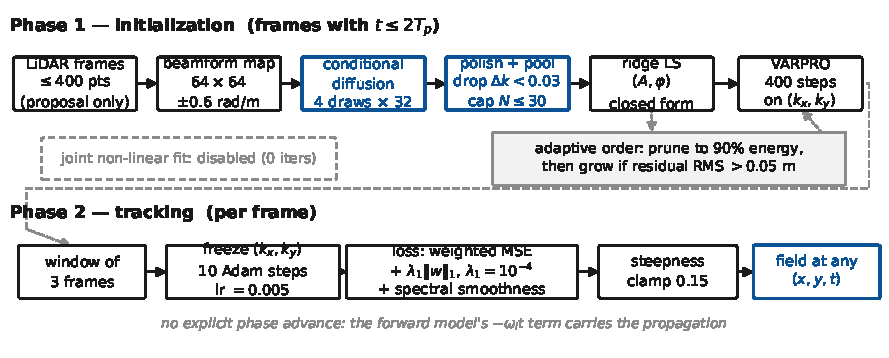
\includegraphics[width=\textwidth]{figures/fig_pipeline_deployed.pdf}
\caption{The deployed pipeline. Phase~1 conditions a diffusion prior on a
coarse beamform map of the initialisation window, draws and polishes candidate
atom sets, pools them into at most $\DepMaxN{}$ atoms, fits amplitude and phase in
closed form, and refines the wavenumbers by variable projection; the adaptive
prune-and-grow step runs before variable projection, on a model that has had no
joint refinement. Phase~2 freezes the wavenumbers and updates $(w_i,\varphi_i)$
over a three-frame window. Blue marks the one learned component, brown the output.
% [2026-09-02 P9] 4차 감사 M1: 캡션이 "two learned components" 인데 파란 상자가 셋이었다.
%   'polish + pool' 도 'field at any' 도 학습이 아니다 ⟹ 색을 분리하고 캡션을 그림에 맞췄다.
The dashed rectangle is a stage that exists in the code and is switched off in the
shipped configuration; the dashed path is the transition between phases. Every
constant printed in this figure is read from the source at generation time by
\texttt{scripts/gen\_fig\_pipeline.py}, which also asserts the four switches that
would change its structure.}
\label{fig:pipeline}
\end{figure*}

\subsubsection{Phase 1: Initialization}
\label{sec:init}

% ============================================================================
% [2026-09-01 P8] BLOCKER 수리. 초판의 이 절은 **해석적 팔**(빔포밍 + coarse-to-fine)
%   만 서술했는데, 개정본 Results 는 그 팔이 학습 사전에 45/48 로 **진다**고 인쇄한다
%   (B-22 L2). 즉 제목·초록이 파는 방법이 논문 어디에도 정의돼 있지 않았다.
%   독립 감사가 잡았다. 배포 경로를 여기 정의하고, 해석적 절차는 **대체 경로**로 강등한다.
%   ⛔삭제하지 않는다 --- 그 절차가 Results 의 절제 대조군(ANA)이기 때문이다.
% ============================================================================

Given the first $T_{\text{init}} = 2 T_p$ seconds of observations, we must place
$N$ atoms in the $(k_x, k_y)$ plane and fit their amplitude and phase. Two
procedures do this in our system, and \emph{which one runs is the subject of one of
our ablations}, so we describe both.

\paragraph{The learned prior: architecture, training data, and what we cannot certify}
% ============================================================================
% ★2026-09-02 (P10) --- 5차 감사의 **reject 경계** 지적:
%   *"제목이 파는 학습 사전을 논문이 두 문장으로 정의한다. 아키텍처.학습 자료.학습 절차가
%    없다 ⟹ 심사자는 재현도 과적합 판단도 할 수 없다. 이것만으로 reject 사유가 된다."*
%   ★아키텍처 수치는 **체크포인트 가중치에서 센다**(손으로 적으면 낡는다).
%   ⚠학습 절차는 배치 문서에서 오고, 그 파일이 **동결 후 움직였다**는 사실을 함께 적는다.
% ============================================================================
The prior is a conditional denoising diffusion model over \emph{sets} of atoms. Its
conditioning branch is a small convolutional encoder that reduces the
$64 \times 64$ beamform map to \PriorTokens{} tokens of width \PriorDim{}
(3$\times$3 convolutions, group normalisation, GELU, with a learned positional
embedding). Its denoiser is a stack of \PriorBlocks{} pre-norm transformer blocks
of the same width: within each block, self-attention over the $32$ atom slots,
cross-attention into the conditioning tokens, and a two-layer feed-forward network.
Atoms enter and leave as three normalised numbers --- two wavenumber components and
a log-energy --- through linear projections, so the model is permutation-equivariant
over the set by construction and has no notion of atom ordering. It has
\PriorParams{} parameters. Sampling is ancestral DDPM with a cosine noise schedule
over $500$ steps, and training is the standard $\epsilon$-prediction mean-squared
error under AdamW (learning rate $2\times 10^{-4}$, weight decay $10^{-4}$, cosine
annealing, batch $32$).

Training scenes are synthetic and are drawn from a deliberately stratified mixture
rather than from the evaluation distribution: discrete crowded ($15$ and $30$
components) at $0.30$, discrete sparse ($1$ and $2$) at $0.20$, five-component at
$0.10$, two continuum strata at $0.10$ and $0.15$, and an intermediate-spreading
stratum at $0.15$, with sea states covering Beaufort~2--5 anchors and a jittered
box around them. The observation geometry used in training is not drawn
independently: frame-structured sweep windows are replayed from \TrainDonors{} donor
episodes, and only the observation coordinates are taken from a donor --- the
surface is always re-rendered from the fresh synthetic scene. That bank of
\TrainDonors{} geometries is small, and it is the only view of sensor geometry the
prior ever had; we note it as a generalisation limit rather than defend it. No donor
episode appears in the frozen result rows of any batch this paper cites (checked
mechanically over all \CitedBatchFiles{} such files).
%   ⛔[2026-09-02] 6차 감사: *"14 geometries is a generalisation fact a referee needs."*
%   실측 확인 = 14 도너 파일명이 `tmp/*/results*.jsonl` 어디에도 없다(런 0회).
\emph{Scene seeds for training are drawn from the band
$[\,\TrainSeedLo{},\; \TrainSeedHi{}\,)$, which is disjoint from every seed used by any
evaluation generator in this paper.} The largest evaluation seed appearing in any
frozen result row of this project is \EvalSeedMax{}. No evaluation episode of any
batch cited in this paper was therefore seen during training, although the generator
family is the same --- which
is the sense in which Section~\ref{sec:res_summary} says only the seed axis is out
of sample.

The shipped checkpoint was trained from scratch for \TrainSteps{} steps at batch
\TrainBatch{} --- \TrainScenes{} scene draws --- against a held-out validation set of
\TrainValScenes{} scenes generated from a separate seed and scored every
\TrainValEvery{} steps. The final losses are \TrainLossFinal{} (training) against
\TrainValLossFinal{} (validation), and the whole curve is in the repository. Two
qualifications belong with that pair. The training figure is a \emph{single
minibatch}, not an average, and neighbouring evaluations straddle it in both
directions, so the apparent gap is not a stable quantity; the validation figure is
stable because it is scored on frozen noise. And ``held out'' here means an
independent random stream --- a separate seed drawing from the same generator, the
same donor bank and the same seed band --- not a set constructed to be disjoint. We
did not use the curve to select a stopping point and no early stopping was applied.
% ⛔[2026-09-02] 검증 감사 MAJOR: 앞 판은 *"the gap is small"* 이라 적었다. `train_mixed.py:129`
%   가 `float(loss)` 를 **한 미니배치**에서 낸다 --- 이웃 평가가 0.0652(38k)·0.0380(39k) 로
%   양쪽에 걸쳐 있어 같은 "gap" 이 2배 넘게도 나온다. 그리고 `make_val` 은 **같은 대역·
%   같은 도너 은행**에서 다른 시드로 뽑으므로 서로소가 **보장되지 않는다**.
% ⛔[2026-09-02] **주석이 본문을 삼켰다** — 아래 한 줄이 그 복구분이다.
The checkpoint's SHA-256 is \texttt{\CkptShaFull{}}. We are precise about
what that digest does: it is recorded in the estimator source and a unit test asserts
that the shipped file matches it, but the loader does \emph{not} check it at run
time, so a reader who substitutes a different checkpoint will not be stopped by the
code.
% ⛔[2026-09-02] 6차 감사 BLOCKER: 앞 판은 *"the estimator **refuses to load** a
%   checkpoint whose SHA-256 does not begin ..."* 라 적었다. **거짓이다** ---
%   `learned_init._load_cond` 는 검사 없이 `torch.load` 하고, `ckpt_sha256()` 은
%   패키지 안에서 **한 번도 호출되지 않는다**. 대조하는 것은 단위 시험 하나뿐이고
%   그것은 `learned_ckpt` 로 넘긴 사용자 체크포인트를 구속하지 못한다.
%   ★수리를 「코드에 검사를 넣기」로 하지 않은 이유: `M7` 배치가 다른 체크포인트를
%   `ckpt=` 로 넘겨 돌린다 --- 하드 거부는 그 경로를 깬다. ⟹ **문장을 참으로 고쳤다.**

Two things about this we cannot certify and will not claim. First, the six training
strata were measured only as a bundle: no ablation isolates what each contributes,
so we cannot say which part of the mixture the prior's behaviour comes from.
% ⛔[2026-09-02] 앞 판은 *"those files have since been modified"* 라 적었다. **틀렸다.**
%   git 확인: 세 파일과 체크포인트와 FROZEN.sha256 이 **같은 커밋**(`c0f89ece`)에 들어갔고,
%   학습 스크립트는 커밋이 **하나뿐**이며 현재 파일이 **커밋본과 바이트 동일**하다.
%   그런데 FROZEN.sha256 의 해시는 셋 다 다르다 ⟹ ★**파일이 표류한 것이 아니라
%   동결 기록이 커밋 시점에 이미 낡아 있었다**(동결 후 편집, 재동결 없이 함께 커밋).
%   방향은 같지만 기제가 다르고, 이 저장소는 그 구분에 반복해 대가를 치렀다.
Second, the batch that produced this checkpoint recorded checksums for its own
training script and preregistration, and those checksums do not match the files that
were committed with them. The files themselves have not drifted --- they are
byte-identical to their single committed version --- so what is missing is not the
code but the guarantee: the freeze was taken, the files were then edited, and the
freeze was never re-taken. The architecture and the checkpoint identity above are
read directly from the shipped weights; every training number above is read
mechanically from that batch's committed artefacts --- its training curve, its
generator source and its run log --- so the recipe \emph{is} reproducible from the
repository. What a reader cannot do is use the freeze certificate to prove that
those artefacts are the ones that produced these weights. That is a weaker defect
than an absent record, and we prefer to name it exactly rather than to describe it
away.
% ⛔[2026-09-02] 6차 감사: 앞 판의 *"not independently verifiable from the repository
%   as it stands"* 는 **과장**이었다 --- 심사자 축자: *"the caveat is being used to
%   excuse omitting facts that are readable in a committed file."* 그 지적이 옳다:
%   이 문단 위의 학습 수치는 이제 전부 `gen_paper_constants._training()` 이
%   `train_curve.json`.`gen_mixed.py`.`train.log` 에서 **기계로 읽는다**.
%   ⟹ 결함은 「기록 없음」이 아니라 「동결이 그 기록을 인증하지 못함」이다.

\paragraph{A dependency we disclose rather than describe away}
% ============================================================================
% ★2026-09-02 (P9) BLOCKER 수리. 초판은 T_p 를 "관측 시계열의 우세 주파수에서 추정"
%   이라 적었다. **거짓이다** --- data_loader.py:45 가 에피소드 HDF5 의 `Tp_true` 를
%   그대로 읽고 run.py:226 이 그 값으로 창을 자른다(get_init_window, tp_factor=2.0).
%   ⟹ 합성 실험에서 초기화 창의 길이는 **참** 첨두주기가 정한다.
%   ⚠판정은 무손상이다: 창은 run.py:226 에서 **팔을 고르기 전에** 한 번 계산돼
%     모든 팔이 같은 프레임을 본다(채점 프레임도 같은 get_tracking_frames).
%     그러나 **배포 현실성**의 문제이고, 숨기면 그것이 결함이 된다.
% ============================================================================
The length of the initialisation window is set by the true peak period of the
episode, read from
the scene metadata, rather than estimated from the observations; on the measured
records it is read from the record's own reported spectrum. This is a property of
the harness and not of any arm: the window is computed once, before an
initialisation procedure is selected, so within a single batch run every arm sees
exactly the same frames, and the scoring frames are chosen the same way. One
comparison in this paper splices its two arms from batches run eight days apart
(B-1), and we checked that case separately rather than assuming it: recomputing the
deterministic scoring-frame rule from each episode reproduces the frame count the
baseline rows recorded, on \BOneFrameMatch{}/\BOneCmpN{} episodes.
% ⛔[2026-09-02] 7차 심사 A2: 앞 판은 *"**every arm in every paired comparison reported
%   here** sees exactly the same frames"* 라 적었다. 그 논거(창을 한 번만 계산한다)는
%   **두 팔이 한 하네스 호출 안에서 돌 때만** 성립한다. `B-1` 은 아니다 ---
%   `W16`(SHIP) 과 `S16`(SPEC25) 두 배치를 이어 붙였고, `S16` 행에는 `n_match` 가
%   {120,160} 로 들어 있는데 `W16` 행에는 **프레임 열이 아예 없다**.
%   ★이것이 코퍼스를 철회시킨 바로 그 결함 부류다. ⟹ 전칭을 좁히고 `B-1` 만 따로
%   **검증**했다: `run.py:263` 의 `get_tracking_frames(tp_factor=2.0)` 을 64 에피소드에
%   다시 돌려 `n_match` 와 대조 = **64/64 일치**.
%   `W16` 러너는 `run_estimation` 을 부르므로 같은 줄(`run.py:263`)을 탄다.
It does mean that a deployment would need to supply $T_p$ from another
source, and that no experiment here measures the sensitivity of the method to
getting it wrong.

\paragraph{What ``the shipped configuration'' selects, and when}
% ============================================================================
% ★2026-09-02 (P9) BLOCKER 수리 --- 논문에 **실측 게이트가 0회** 등장했다.
%   `sequential_update.py:775-812`: `init_method='auto'` 는 프레임에 비퇴화 GT 필드가
%   없으면(`_frames_have_gt`, `:411-427`) `real_estimator`(출하 `bank_mmse`, `run.py:81`)
%   로 **경로를 통째로 갈아탄다** --- `_initialize_learned` 에 들어가지도 않는다.
%   ⟹ 표 3 캡션의 *"the deployed estimation pipeline"* 은 **합성 입력에서만** 참이었다.
%   ⚠경계 표(Table 6)의 행들은 학습 팔을 **명시 강제**해서 잰 것이다(동결 행 되읽기:
%   B-17 `init_method='learned'` 18/18 · B-18 30/30). ⟹ 그 사실을 적어야 한다.
% ============================================================================
The router that selects an initialisation procedure is not purely a quality
heuristic: it also branches on whether the input carries a ground-truth field.
When none is present --- which is the case for every measured record --- the
shipped configuration switches to a separate estimator built around a bank of
candidate spectra, and the learned path described above is not entered at all.
Table~\ref{alg:wavesplat} therefore describes what runs on the synthetic corpora.
The measurements that report no skill on the measured records
(Section~\ref{sec:res_scope} and Table~\ref{tab:boundary}) were obtained by
\emph{overriding} that router and forcing the learned path, because the question those batches ask is what the learned prior does
on real data, not what the shipped default does. % ⛔[2026-09-02] 적대적 심사 B-1(BLOCKER): 이 자리의 전칭 *"none of its results are
%   reported here"* 는 **같은 날 오후에 거짓이 됐다** --- 개명 직후 넣은 실측 그림 두 장이
%   bank 팔의 실측 결과를 인쇄한다(`fig:real` 범례 · 패널 (b) · `fig:real_qual` (c)(e)).
%   ★전칭을 두고 뒤에 반례를 추가한, 이 원고가 반복해서 대가를 치른 그 부류다.
The bank estimator is not a contribution of this
paper and no result of it supports any claim made here. It does appear, as the
deployed reference arm of Figs.~\ref{fig:real} and~\ref{fig:real_qual}, where it is
scored against its own per-record zero-field reference and not against the learned
arm; that is a disclosure about where the shipped configuration actually sends
measured input, not a result we claim. We state its existence because a reader
reproducing ``the shipped configuration'' on a real record would otherwise get a
different algorithm than the one we describe.

% ⛔[2026-09-02] 적대적 심사 m-2: 제목의 대상을 **정의하는** 이 절과 §5·결론에
%   `WavePrior` 가 **0회**였다(전수 grep: 출현 8회가 전부 frontmatter·§1·§6.6).
\paragraph{Deployed path: the learned set-valued prior (WavePrior)}
The configuration evaluated in Section~\ref{sec:results} places the atoms with a
learned prior over wavenumber--energy \emph{sets}. A conditional diffusion model,
trained on synthetic scenes, is conditioned on the initialisation-window
% [2026-09-01] 2차 감사: 코드는 merge 가 아니라 **drop** 이다(learned_init.py:184).
%   merge_atoms 는 별도 기능이고 기본 no-op 이며 W-4 가 무익을 측정했다.
% [2026-09-02 P9] 4차 감사 MINOR 둘: ①코드 순서는 **에너지 문턱이 먼저**이고
%   dedup 이 나중이다(`learned_init.py:179-184`) --- 표 3 은 옳게 적었고 이 산문만 뒤집혔다.
%   ②판정은 유클리드 거리가 아니라 **축별 상자**다(`abs(dkx)<dk and abs(dky)<dk`).
% ⛔[2026-09-02] 6차 감사 N2: 4차 감사가 **순서**를 고치면서 새 절을 아래에 덧붙이고
%   낡은 "deduplicated in wavenumber" 를 **지우지 않았다** ⟹ 인쇄면에 같은 절이 두 번
%   나오는 비문이 됐다. ★"고쳐 쓴 문장을 넣었으면 낡은 것을 지워라"(N-1 부류).
% ⚠[2026-09-02] 주석 블록을 **문장 중간에서 위로** 옮겼다 --- `check_comment_swallow.py`
%   가 문장 중간 주석과 「주석이 삼킨 본문」을 구별하지 못하기 때문이다.
%   ★가드가 잡을 수 있게 쓰는 것이 가드를 느슨하게 하는 것보다 낫다.
observations and draws several posterior samples of an atom set; the pooled draws
are then thresholded on energy, then deduplicated in wavenumber (an atom is dropped when a
higher-energy atom lies within $\Delta k = 0.03$~rad/m of it \emph{on both axes}),
and truncated at $N_{\max}$. Given the resulting
wavenumbers, the amplitude and phase of every atom are obtained in closed form by
ridge-regularised least squares, and the whole set is refined by \emph{variable
projection}: because the model is linear in $(a_j, b_j)$ once $(k_{x,j}, k_{y,j})$
are fixed, the linear coefficients can be eliminated analytically and only the
wavenumbers are iterated.

% [2026-09-02 P9] 코드 감사 D8. 체크포인트에서 직접 읽었다: stats['K_LIM'] = 1.1.
%   샘플러가 마지막에 clamp(-1,1) 하므로 |kx|,|ky| <= K_LIM 이 **구조적 상한**이다.
%   ⚠논문에 이 상한이 한 번도 적혀 있지 않았다.
The learned proposal cannot place an atom outside a bounded region: the network
emits normalised coordinates that are clipped to $[-1,1]$ and rescaled by a
constant that lives in a \emph{second} checkpoint. The deployed learned path loads
two files: the conditional denoiser identified above, and an earlier unconditional
set-diffusion checkpoint (\texttt{setdiff\_prior.pt}, SHA-256
\texttt{\PriorCkptSha{}}) from which it reads the normalisation constants that the
two models share. The rescaling constant is one of these, giving
$|k_x|, |k_y| \le \DepKLim{}$~rad/m. For
the sea states evaluated here the largest true wavenumber is near $1.0$~rad/m, so
the bound is satisfied with little margin, and it is a property of the checkpoint
rather than of the representation --- the analytic alternative searches
$\pm \DepAnaKMax{}$~rad/m.
% [2026-09-02 P9] 4차 감사 M14: 실제로 **구속력 있는** 상한은 clip 이 아니라 **조건화 지도**다.
%   `d3_beamform_net.py:31 KLIM = 0.6` --- 신경망이 자료를 보는 유일한 통로가 ±0.6 이다.
A tighter bound applies upstream: the only view of the data the network receives is
the conditioning periodogram, and that grid spans $\pm 0.6$~rad/m. Components with
$|k|$ between $0.6$ and the clip bound are therefore outside the network's input
entirely, and can be reached only by the residual-growth step, whose beamformer does
search the wider range. We have not measured how often that happens. Any application to shorter waves would need the prior retrained,
and we have not measured what happens when a true component lies outside the
bound.

Two deployment choices matter for reproducing the numbers in this paper. Variable
projection is enabled ($\DepVarproSteps{}$ steps); and the joint non-linear fit that
earlier versions ran after initialisation is \emph{disabled} ($\DepJointFitIters{}$ iterations) --- it was measured to be
redundant once variable projection is present. These two are not independent:
removing the joint fit leaves a larger residual, which in turn makes the adaptive
growth rule of Section~\ref{sec:adaptive_order} fire far more often than it did
before.
% [2026-09-02 P9] ★미사용 매크로 검사가 드러낸 것: 배포 설정이 이고 다니는 스위치 하나가
%   **이 경로에서 구조적으로 무연산**인데 논문에 그 말이 한 줄도 없었다.
%   근거: `sequential_update.py` 의 `_effective_k` 가 **해소된 경로**로 k 를 다시 읽는다.
A third value in the shipped configuration is worth naming because it is
\emph{inert}: the configuration sets an analytic-path ensemble of
\DepAnalyticEnsK{}, but the router resolves to the learned path and the ensemble
size is then re-read for the resolved route, which ships at \DepLearnedEnsK{}. No
median-of-$k$ ensemble therefore runs in the shipped configuration. Two places in
this paper report results that do use one, both deliberately: the two S-ENS rows of
Table~\ref{tab:earns}, and the analytic comparator of the W-15 re-aggregation in
Section~\ref{sec:res_scope}, whose package is the analytic path \emph{with} its
ensemble intact.
% ⛔[2026-09-02] 7차 심사 B2: 오늘 아침 이 전칭에 S-ENS 예외를 달았는데 **형제를
%   놓쳤다** --- `gates_w15.py` 의 `ALL-ANALYTIC` 은 해석적 경로 **k=3** 이고 §5.6 이
%   그것을 *"with that package's ensemble intact"* 라 적는다. ★N−1 의 재발.
We say
so because a reader inspecting the configuration file would reasonably conclude
otherwise.
% ⛔[2026-09-02] 검증 감사 BLOCKER: 이 문장은 *"any synthetic result reported here"* 라는
%   **전칭**이었고 **표 5 의 S-ENS 두 행이 반증**한다(그 행이 바로 앙상블을 켠 대조다).
%   ★오늘 전칭으로 틀린 것이 네 번째다.
% ⛔[2026-09-02] **주석이 본문을 삼켰다** — 아래 한 줄이 그 복구분이다.
We note this because it is easy to reason about either switch alone and be
wrong about the resulting system.

\paragraph{Alternative path: dispersion-aware beamforming}
The system also contains a purely analytic initialiser, which is what runs when the
learned prior is not used. It is described next both because it is the fallback and
because it is the \emph{comparison arm} of the prior ablation in
Section~\ref{sec:res_ablation}: replacing the learned proposal with this procedure,
changing nothing else, is what accounts for a margin of \BTwentyTwoRel{} --- against an analytic package that itself
clears a zero predictor, though thinly (\BTwentyTwoAnaShipZero{}/\BTwentyTwoN{}, $p = \BTwentyTwoAnaShipZeroP{}$).

\textbf{Dispersion-aware beamforming.}
Initial wavenumber estimates are obtained by scanning a Cartesian
grid in wavenumber space.  The grid covers
$k_x, k_y \in [-4.0, 4.0]$~rad/m with $81 \times 81$ bins
(resolution $\Delta k \approx 0.10$~rad/m), spanning wavelengths
from $\sim$1.6~m to $\sim$130~m and encompassing Beaufort~2--5
conditions at $d$=50~m depth.  The search bound of 4.0~rad/m
is set conservatively above the highest wavenumber component
present in the dataset ($|k|_\text{max} \approx 1.0$~rad/m for
BF3--5 sea states), ensuring full coverage with margin.

For each candidate $(k_x, k_y)$, we compute
$\omega = \sqrt{g|k|\tanh(|k|d)}$ and evaluate the beamforming power:
\begin{equation}
  P(k_x, k_y) = \left| \sum_{j} z_j \, e^{-i(k_x x_j + k_y y_j - \omega t_j)} \right|^2
\end{equation}
where the summation runs over all observations accumulated during
$T_\text{init}$.  The use of the dispersion-derived $\omega$ means
that the beamforming naturally filters for physically plausible
wave signals, suppressing noise that does not lie on the
dispersion surface in $(k_x, k_y, \omega)$ space.

Peaks in $P$ are extracted greedily: the maximum is selected, then
all candidates within a Cartesian radius of 0.15~rad/m are
suppressed, and the process repeats.  The 0.15~rad/m threshold
prevents double-counting of the same wave component spread across
adjacent wavenumber bins, while being narrow enough to resolve
crossing sea systems.  The initial amplitude and phase of each extracted component
are estimated via linear least-squares projection of the accumulated
observations onto the selected wavenumber basis functions.

Each extracted peak is then refined locally via a second beamforming
pass on a finer $41\times41$ grid spanning $\pm0.2$~rad/m around
the coarse peak ($\Delta k_{\text{fine}} = 0.01$~rad/m), improving
wavenumber accuracy from $\sim0.10$ to $\sim0.01$~rad/m. Without
this refinement, the 0.10~rad/m coarse grid would limit $|\mathbf{k}|$
accuracy to roughly 17\% at typical BF4 wavenumbers
($|\mathbf{k}| \approx 0.6$~rad/m), inducing significant phase
drift during subsequent tracking.

\textbf{Coarse-to-fine optimization.}
Starting from the beamforming initialization, we optimize the
spectral parameters in three stages ($N$=3 $\to$ 8 $\to$ 15),
with up to 200/200/500 iterations of the Adam optimizer~\citep{kingma2015}
(learning rate $\text{lr} = 1 \times 10^{-2}$,
$\beta_1 = 0.9$, $\beta_2 = 0.999$) at each stage.
The loss function is:
\begin{equation}
  \mathcal{L} = \underbrace{\frac{1}{M} \sum_j c_j \, (z_j - \hat{z}_j)^2}_{\text{weighted MSE}}
    + \underbrace{\lambda_1 \sum_i |w_i|}_{\text{sparsity}}
    + \underbrace{\lambda_s \sum_i (w_{\sigma(i)} - w_{\sigma(i-1)})^2}_{\text{spectral smoothness}}
\end{equation}
% [2026-09-01] 2차 감사: 손으로 적힌 10^{-3} 은 2026-08-11 이전 값이고 배포는 1e-4 다.
%   ⟹ 매크로로 바꾼다(gen_paper_constants.py 가 코드에서 생성).
where $\lambda_1 = \DepLambdaOne{}$ promotes amplitude sparsity (driving
negligible components toward zero for subsequent pruning) and
$\lambda_s = 10^{-4}$ penalizes abrupt amplitude variations between
spectrally adjacent components ($\sigma$ denotes ordering by $|k|$),
encouraging smooth spectral envelopes consistent with JONSWAP-like
spectra.

During optimization, wavenumber components $(k_{x,i}, k_{y,i})$
are free parameters (unlike in the tracking phase).  The dispersion
constraint is enforced by computing $\omega_i$ from $(k_{x,i}, k_{y,i})$
at each forward evaluation rather than treating $\omega_i$ as a free
parameter, ensuring that the constraint is satisfied exactly
throughout optimization.

\subsubsection{Adaptive model order}
\label{sec:adaptive_order}

After initialization, we apply energy-based pruning.
Components are sorted by energy $E_i = w_i^2$ in descending order,
and the minimum set capturing 90\% of total energy
$\sum_i E_i$ is retained.  This criterion is motivated by the
JONSWAP spectral shape, where a small number of components near the
spectral peak typically contain the majority of the wave energy.

A safety check prevents aggressive pruning from discarding physically
significant components: if the post-pruning RMSE exceeds
130\% of the pre-pruning value, pruning is rolled back entirely.
This can occur when two components of similar energy
contribute to different spatial regions (e.g., crossing seas),
making each individually appear low-energy.

If the residual RMS after pruning exceeds $\tau_R = 0.05$~m
(indicating unmodeled wave energy), new components are grown by
applying beamforming to the residual signal $r_j = z_j - \hat{z}_j$
and adding the dominant residual peaks to the model, up to
$N_{\max}=30$. Grown components are initialized via this residual
beamforming step and are not re-run through the full $N$=3$\to$8$\to$15
coarse-to-fine schedule, trading some initialization quality for
computational efficiency at this stage.
The threshold is derived from the theoretical
% SCOPE 2026-08-14: the "Gerstner--linear model mismatch" term in this budget is not
% present in the synthetic corpus (measured mismatch 0.000e+00) -- it is an allowance
% for real waves. The threshold itself is unchanged; only its justification narrows.
% (basis: memory/project_audit_recheck_2026-08-13.md section 6.5)
residual floor: combining LiDAR range noise ($\sigma_r \approx
0.02$~m) with a nonlinear--linear model mismatch allowance at BF4
($O(\epsilon^2)\,H_s/2 \approx 6$~mm; this term is
an allowance for real waves and is \textbf{absent} in the synthetic corpus,
where the measured mismatch is zero) and angular-noise projection
(${\sim}5$~mm) yields a lower-bound RMS of ${\sim}0.022$~m;
$\tau_R = 0.05$~m provides a ${\sim}2.3\times$ safety margin for
unambiguous detection of unmodeled signal.
A caveat here belongs to a rendering that this paper no longer uses. On the
\emph{superseded} 40$\times$30 mesh, the mesh's own facet-rendering error contributed
comparably to this budget (mean ${\approx}0.048$~m for BF3--BF5 multi-component
scenes, versus the ${\sim}0.022$~m physical floor above), so part of what triggered
residual-based growth there may have been rendering error rather than unmodeled wave
content. The corpora used here are rendered at 200$\times$167
(Section~\ref{sec:experiments}), whose spacing is adequate for every component present;
\emph{we did not re-measure the facet-rendering error on that mesh}, so we state the
old figure as a property of the old rendering and leave the re-validation of $\tau_R$
open.
% ⛔[2026-09-02] 7차 심사 B7: 이 문단이 *"the raycast-mesh-rendered dataset **used
%   throughout this paper** ... on the **shipped 40x30 mesh**"* 라 적었다. §4.2 는
%   코퍼스를 **200x167** 로 재생성했다고 적는다(6쪽 뒤). ⟹ 낡은 값을 **낡은 렌더링의
%   성질**로 명시하고, 재측정하지 않았음을 밝힌다.
We also note that $\tau_R$ is an \emph{absolute} residual RMS in metres,
compared without normalization by sea state, so its effective strictness
varies with $H_s$; a scale-invariant form that normalizes the residual by
the observed signal RMS is implemented but not enabled by default.
A sensitivity sweep over $\tau_R \in \{0.02, 0.05, 0.08, 0.10, 0.15\}$~m
on 12 representative episodes of the retracted corpus found no ordering among the
values in $[0.05,\,0.15]$~m, while $\tau_R = 0.02$~m caused over-growth in
multi-component seas. The per-value levels
from that sweep are not quoted: it was run on the retracted corpus and before the
tracker phase-advance correction, and no re-measured substitute exists. % ✅[2026-09-02] 전칭 검증: 인용 배치 **11개** 어디에도 `grow_residual_threshold` 를
%   재지정하는 코드가 없다(`grep -rl` 전건 0) ⟹ 배포 기본값 0.05 가 그대로 쓰였다.
The value
$\tau_R = 0.05$~m has been held fixed in every batch reported here.

% [2026-09-02 P9] fig:tau 를 아카이브로 옮겼다 --- 12에피소드 스윕이 철회된 코퍼스다.
%   ⛔대체 없음 ⟹ 그림을 옮기고 그 자리에 수치를 다시 적지 않는다.

\subsubsection{Phase 2: Tracking}

% ============================================================================
% ★2026-09-02 (P9) BLOCKER 수리 --- 이 절이 **같은 논문의 표 3 과 모순**이었다.
%   초판은 "Predict: phi += omega*dt … This prediction is exact" 를 배포 사이클의
%   1단계로 적었는데, `sequential_update.py:351 TRACK_PHASE_PREDICT = False` 이고
%   `:1429` 가 그 상수로 막혀 있다 ⟹ **그 단계는 돌지 않는다**(2026-07-26 에 꺼졌다).
%   표 3 은 세 문단 뒤에서 "no explicit phase advance" 라 정확히 적고 있었다.
%   ★코드 대조 감사가 잡았다. ⟹ 또 하나의 「철회가 N-1 에서 멈춘」 사례.
% ============================================================================
For each subsequent LiDAR frame we perform a single update step. There is no
explicit predict step: an earlier version advanced the phases by
$\varphi_i \mathrel{+}= \omega_i \Delta t$ before each update, but that path is
switched off in the shipped configuration and the forward model's own
$-\omega_i t$ term carries the propagation instead, with $t$ the absolute frame
time. The update performs $K=\DepTrackingSteps{}$ Adam steps
(lr~$=\DepTrackingLr{}$) on the weighted MSE loss over a sliding window of
$K_w=3$ recent frames, updating only amplitudes $w_i$ and phases $\varphi_i$ while
freezing wavenumbers $(k_{x,i}, k_{y,i})$ (\texttt{w\_phi} tracking mode).

Freezing wavenumbers during tracking is motivated by two considerations.
First, wavenumber estimation from a single frame is ill-conditioned: the LiDAR's
irregular sampling does not constrain the wavenumber from one snapshot, whereas
the initialisation window spans $2T_p$, which at $10$~Hz and the peak periods used
here is on the order of one to two hundred frames.
% [2026-09-02] 초판은 여기에 "~20 frames" 라 적었다. 2*Tp/0.1s 는 Tp=4-9s 에서
%   80-180 프레임이다 --- 4-9배 어긋난다. 코드 대조 감사가 잡았다.
Second, with the wavenumbers fixed the per-frame problem is linear in a small
number of parameters, so a short optimiser budget suffices.
% [2026-09-02] 초판의 "~200 (full optimization) to 10" 은 **해석적 팔**의 단계별
%   반복 예산이었다. 배포 경로의 Phase 1 은 결합 적합이 0 회이므로 비교 대상이 없다.

The sliding window ($K_w = 3$) uses the three most recent frames
for gradient computation.  This provides temporal averaging that
smooths single-frame noise without introducing excessive latency:
at 10~Hz, the window spans 0.3~s, much shorter than the peak
period $T_p$ for all sea states considered.

\subsection{Computational complexity}
\label{sec:complexity}

Let $M$ denote the number of LiDAR observations per frame and
$N$ the number of spectral components.

\textbf{WaveSplat}: Each forward evaluation computes
$z(x_j, y_j, t) = \sum_{i=1}^{N} w_i \cos(\cdot)$,
costing $O(M \cdot N)$ per frame. With $K$ gradient steps and window
size $K_w$, the per-frame tracking cost is $O(K \cdot K_w \cdot M \cdot N)$.
% RETRACTED/CORRECTED 2026-08-14: (a) 13.4 ms/frame is a banned figure -- it comes from
% a separate-process timing comparison; (b) the CPU is AMD Ryzen 7 7800X3D, not
% Intel i7-12700H (banned since 2026-08-05).
% (basis: memory/reference_citation_bans.md (08-05), (08-13 round 3))
% --- original (kept for history) ---
% In practice, $K{=}10$, $K_w{=}3$, $N \leq 30$, yielding 13.4~ms/frame
% on CPU (single-threaded, Intel i7-12700H).
In practice, $K{=}\DepTrackingSteps{}$, $K_w{=}3$, $N \leq \DepMaxN{}$, measured on
CPU. An earlier absolute per-frame figure quoted here was withdrawn as a
cross-process timing (\ref{app:changes}, R3); the measured replacement is
below.

% ============================================================================
% ★2026-09-02 (P9) --- 코드 대조 감사 (c). 이 절은 **Phase 2 만** 특성화한다.
%   그것은 초판부터 그랬고 그때는 Phase 1 이 격자 탐색 + Adam 이라 큰 문제가 아니었다.
%   지금 배포 Phase 1 은 500스텝 역확산 x4 + 폴리시 80x4 + VARPRO 400 이다
%   ⟹ **지배적 비용이 특성화되지 않은 채 남아 있다.** ⛔대체 수치가 0개라 만들지 않는다.
% ============================================================================
% ============================================================================
% ★2026-09-02 (P10) --- `T6-BUDGET`. 이 문단은 어제까지 *"배포 초기화 비용의 측정이
%   없다"* 고 적었고 그것이 5차 감사의 MAJOR #3 이었다. 이제 측정이 있다.
%   ⛔같은 세션에서 「내가 쓴 문장이 다음 측정으로 거짓이 되는」 부류의 세 번째다.
% ============================================================================
\emph{This analysis covers the tracking phase only.} It is unchanged by which
initialisation ran, because the tracking loop does not branch on the initialiser,
and we verified that: across a pre-registered $64$-run batch spanning two
initialisation routes, two strata, and CPU-only versus GPU-available execution, the
per-frame tracking cost varied only between \FrameMsMin{} and \FrameMsMax{}~ms.

\paragraph{Measured budget}
Table~\ref{tab:budget} gives the whole batch rather than a summary of it. The cell
the preregistration named as the reporting cell --- CPU-only, crowded, one thread ---
costs \FrameMsLearn{}~ms per tracking frame, or \FramePctLearn{}\% of a $10$~Hz
budget, with initialisation a one-off \InitSLearn{}~s. We are precise about the word
\emph{reporting}: the preregistration called that cell ``the most conservative'', and
the measurement does not bear that label out. All eight cells lie between \FrameMsMin{} and \FrameMsMax{}~ms and the
reported cell is the fastest of the eight, so it should be read as the cell fixed in
advance, not as a worst case. The spread across the table is the substantive point ---
a factor of \FrameMsSpread{} between the extreme cells --- and it is why the tracking analysis above does
not branch on which initialiser ran.

Two rows run against the intuition a reader may bring. The learned initialiser is
\emph{faster} than the analytic alternative, not slower --- \InitSLearn{}~s against
\InitSAna{}~s on the same episodes --- despite running a $500$-step reverse diffusion
sampler four times; we report the direction and do not attribute it. And a GPU buys
almost nothing: the same initialisation takes \InitSLearnGpu{}~s with one available,
and every GPU row is marginally \emph{slower} per frame than its CPU counterpart.
No number here is comparable with any latency in the earlier version of this paper,
which came from separate processes, and the batch did not run a baseline arm, so no
comparative timing claim is available.
% ⛔[2026-09-02] 6차 감사 N16 + 권고 8. 두 가지가 한 번에 고쳐진다:
%   ①*"the most conservative cell"* --- 사전등록의 **사전 라벨**이었고 측정이
%     그것을 지지하지 않았다(그 칸이 여덟 중 **가장 빠르다**). 검사기 규칙
%     `예산-보수적칸` 은 그 **자구가 있는지**만 봤지 **참인지**를 보지 않았다.
%   ②*"prints 5 of ~32 numbers as prose"* --- 표를 만들었다(`gen_budget_table.py`).
% ⛔자동 생성 — 손으로 고치지 마라.
%    생성: python3 scripts/gen_budget_table.py   (런 0회, T6 동결 verdict 재인쇄)

\begin{table}[!htbp]
\centering
\footnotesize
\caption{Measured cost of the deployed estimator, one process, one thread, on an AMD Ryzen~7 7800X3D. Every cell is \(8\) episodes; the per-frame column is the median over episodes of the per-episode median frame, with the interquartile range (the batch takes the upper median of an even sample, `sorted(v)[n//2]`), and the budget column is that value against a \(10\)~Hz frame interval. Initialisation is a one-off cost and is not part of the per-frame figure. \emph{No baseline arm was run in this batch}, so no comparative timing claim follows from it, and these numbers are not commensurable with the cross-process figures withdrawn in \ref{app:changes}, R3. Pre-registered as T-6; all ten gates pass, including a per-run read-back that the thread count was one and that the shipping constants were in force. This batch runs one estimator seed, unlike the accuracy batches, which use three; timing is not averaged over seeds.}
\label{tab:budget}
\setlength{\tabcolsep}{5pt}
\begin{tabular}{lllrrr}
\toprule
Device & Init.\ path & Stratum & Frame [ms] & \(10\)~Hz budget & Init.\ [s] \\
\midrule
CPU & learned & crowded & 5.91 {\scriptsize[5.85,6.07]} & 5.9\% & 5.18 \\
CPU & learned & sparse & 5.95 {\scriptsize[4.92,6.01]} & 5.9\% & 5.89 \\
\addlinespace[2pt]
CPU & analytic & crowded & 6.05 {\scriptsize[5.87,6.08]} & 6.0\% & 26.61 \\
CPU & analytic & sparse & 5.97 {\scriptsize[5.91,5.99]} & 6.0\% & 17.08 \\
\addlinespace[2pt]
GPU & learned & crowded & 6.20 {\scriptsize[6.12,6.24]} & 6.2\% & 4.86 \\
GPU & learned & sparse & 6.06 {\scriptsize[5.08,6.15]} & 6.1\% & 4.30 \\
\addlinespace[2pt]
GPU & analytic & crowded & 6.26 {\scriptsize[6.17,6.28]} & 6.3\% & 27.57 \\
GPU & analytic & sparse & 6.12 {\scriptsize[6.05,6.15]} & 6.1\% & 17.48 \\
\bottomrule
\end{tabular}
\end{table}


% ============================================================================
% ★2026-09-02 (P9) --- 4차 감사 B9 의 나머지 절반.
%   ⛔프로세스간 지연은 전부 철회됐지만, **질의 렌더 단가**는 다른 양이고 실제로
%   측정돼 있다(`B-6b`, 게이트 6/6, 세 레코드 R^2 >= 0.9991, 동결 verdict).
%   ⚠병기 의무 2건: (i) **격자 기반 실측 경로**의 계측이고 학습 렌더러로는 재측정되지
%   않았다 (ii) **초기화 이후 정상 상태**만 포괄한다(제안 단계 불포함).
%   ⟹ 학위논문은 이 값을 싣고 있었는데 논문에는 없었다.
% ⛔[2026-09-02] `db356491` 이 위에 `\paragraph{Measured budget}` 을 끼워 넣으면서
%   이 문장을 고아로 남겼다 --- 그 커밋 메시지 자신이 *"네 번째 재발"* 이라 적고 셋을
%   고쳤는데, **이것이 다섯 번째**다.
\paragraph{A second, query-side timing}
Evaluating the estimated field at a point costs \BudgetUsPerPoint{}~$\mu$s, linear
in the number of query points over the measured range, so a
\BudgetFrameS{}~s frame budget admits of order several hundred query points. Two
caveats travel with that number and neither is small: it was measured on the
grid-based path used for the measured records and has \emph{not} been re-measured
with the learned renderer, and it covers the steady state after initialisation
only, so the proposal stage --- four diffusion draws of $500$ reverse steps each,
plus polish --- is not in it. It is a budget for querying a field one already has,
not a latency for producing one.

\textbf{ETKF-grid}: The Ensemble Transform Kalman Filter maintains
$N_e$ ensemble members on a $G_x \times G_y$ spatial grid.
Each update involves FFT-based propagation at
$O(N_e \cdot G_x G_y \cdot \log(G_x G_y))$ plus the ensemble
% RETRACTED 2026-08-14: "132.6 ms/frame as the ETKF cost" is on the citation-ban list
% (separate-process timing). (basis: memory/reference_citation_bans.md (08-05),(08-13))
% --- original (kept for history) --- ... this yields 132.6~ms/frame.
transform at $O(N_e^3 + N_e^2 \cdot M)$. The tuned configuration is
($N_e{=}100$, $G{=}40 \times 30$); see Table~\ref{tab:complexity}.
No absolute latency is quoted for this arm: the earlier figure was withdrawn as a
cross-process timing (\ref{app:changes}, R3) and no baseline arm has been
re-timed.

\textbf{GPR}: Gaussian Process Regression with $M$ observations
requires $O(M^3)$ for Cholesky factorization, making it impractical
for dense LiDAR data; kernel hyperparameter optimisation dominates the per-frame
cost.
% ⛔[2026-09-02] 7차 심사 B5: 여기 있던 *"Even with 50 points/frame, per-frame fitting
%   **exceeds 200 ms**"* 는 부록 `R3` 이 철회한 **절대 프레임 지연**의 한 사례다.
%   같은 절이 세 문장 앞에서 *"No absolute latency is quoted for this arm"* 이라 적는다.
%   ★같은 값이 표에서는 지워졌고 산문에만 남아 있었다(N−1).

Table~\ref{tab:complexity} summarizes the scaling comparison.

\begin{table}[t]
\centering
\caption{Asymptotic per-frame cost.
$M$: observations/frame, $N$: spectral components,
$G$: grid size, $N_e$: ensemble members.
ETKF uses the tuned configuration ($N_e=100$, $G=40\times30$).
This table is analytic only. It carried a measured column in earlier versions; those
figures were withdrawn as cross-process timings (\ref{app:changes}, R3), and the
same-process replacement measured since covers our own arm alone and is reported
separately in Table~\ref{tab:budget}. We do not place our measured arm beside
un-timed baselines in one column, because a reader would read a comparison that was
never run.}
\label{tab:complexity}
% ⛔[2026-09-02] 6차 감사: `[retracted]` 마커 **세 개**가 한 열에 서 있었다.
%   ★그 열은 이제 **존재하지 않는다** --- 우리 팔의 측정은 표 `tab:budget` 로 갔고,
%   기준선은 재계측되지 않았다. 「빈 열 + 마커」보다 「열 없음 + 문장」이 정직하다.
%   ⛔기준선 칸을 우리 수로 채우고 싶은 유혹의 반대 방향으로 고친 것이다.
% --- original measured column (kept for history) ---
% WaveSplat & ... & 13.4~ms \\  ETKF-grid & ... & 132.6~ms \\  GPR & ... & $>$200~ms \\
\begin{tabular}{lc}
\toprule
Method & Per-frame complexity \\
\midrule
WaveSplat & $O(K \cdot K_w \cdot M \cdot N)$ \\
ETKF-grid & $O(N_e \cdot G^2 \log G^2)$ \\
GPR       & $O(M^3)$ \\
\bottomrule
\end{tabular}
\end{table}

% ============================================================================
\section{Experimental Setup}
\label{sec:experiments}

\subsection{Simulation environment}

We develop a physics-based LiDAR wave simulation (WaveSim) generating
ground-truth wave fields with JONSWAP spectrum
sampling~\citep{hasselmann1973}.  The simulator parameters are:
\begin{itemize}
  \item \textbf{Sea states}: Beaufort~2--5
    ($H_s$=0.3--2.0~m, $T_p$=4--9~s)
  \item \textbf{Wave complexity}: 1, 2, 5, 15, 30 spectral components
    with directional spreading ($\pm 20^\circ$)
  % RETRACTED/CORRECTED 2026-08-14: the ground truth is NOT nonlinear. The generator
  % calls evaluate_field(), which is
  %   `_, _, Z, NX, NY, NZ = single_gerstner(...)` (wavesim/gt_generator.py:38)
  % -- the two horizontal displacement components are discarded, and
  % wavesim/pipeline.py:157,165 build BOTH the ground-truth field and the raycast mesh
  % from that function. Reconstructing the stored gt_wave_field as a plane-wave sum gives
  % max|delta| = 0.000e+00 on four episodes across sparse, crowded and public corpora.
  % Nonlinear validation was performed in a separate HOS (M=3) batch, not on this corpus.
  % (basis: memory/project_audit_recheck_2026-08-13.md section 6.5 ·
  %  memory/project_hosgate_result_2026-08-13.md · direct code reading 2026-08-14)
  % --- original (kept for history) ---
  % \item \textbf{Ground-truth wave model}: Gerstner waves (nonlinear),
  %   providing a realistic test of the linear forward model~\eqref{eq:forward}
  \item \textbf{Ground-truth wave model} (\ref{app:changes}, R2): The synthetic ground truth is a \emph{displacement-free
    linear superposition on a fixed grid}: the generator discards the
    horizontal displacement components of the Gerstner solution, so the
    ground truth lies in the \emph{same function space} as the estimator's
    model equation. Nonlinear validation was carried out in a separate
    higher-order-spectral ($M{=}3$) batch, not on this corpus.
  \item \textbf{LiDAR model}: 500 horizontal beams per scan,
    10~Hz scan rate, range 10--250~m.  The beam count represents the
    total number of ray directions per frame (horizontal fan);
    real-world solid-state LiDARs such as the Seyond Falcon~K1
    (1550~nm, 152 vertical channels, $120^\circ \times 25^\circ$ FOV)
    produce comparable or higher point densities per scan
  \item \textbf{Raydrop models}: two return-sampling patterns that differ
    in how return density is distributed over range and incidence angle.
    (a)~\emph{Geometry-weighted}: retention probability
    $P\propto R_{\text{Fresnel}}(\theta)\cos\theta/d^2$, so near-range,
    near-normal facets are preferentially retained.
    (b)~\emph{Unweighted}: each ray hit is retained with equal
    probability, calibrated to the same expected return count.
    We retain the historical labels ``uniform'' and ``slope'' for
    these two models for consistency with the released dataset.
    The second model was originally specified as a specular-backscatter
    channel, but that channel is unreachable at the grazing incidence
    angles of a mast-mounted LiDAR: retro-specular return requires the
    ray to strike within $\alpha/2 = 2.5^\circ$ of the surface normal,
    whereas the beam fan spans $78$--$90^\circ$ from vertical and wave
    slopes reach only ${\sim}7^\circ$ at BF7.  The implementation
    consequently always takes its unweighted fallback path, which is
    what we describe and report here.  The contrast is therefore a test
    of sensitivity to the \emph{spatial weighting} of returns, not of
    diffuse versus specular optics
  \item \textbf{Water depth}: $d = 50$~m (intermediate to deep water
    for the wavelengths considered)
\end{itemize}

Each episode contains 301 frames (30~s at 10~Hz) with ground-truth
elevation fields evaluated on a 80$\times$60 spatial grid
covering the LiDAR observation area.
A total of 100 episodes are generated across 5 random seeds per
configuration.
% [2026-09-02 P9] 4차 감사 M7: 이 문단은 **지금 논문에 없는 설계**를 서술하고 있었다
%   (5지표 평가 · 12에피소드 분해 · 100짝 Wilcoxon). 셋 다 철회 코퍼스 산물이고
%   개정본 Results 에는 하나도 없다. ⟹ 실제로 쓰인 방식으로 대체한다.
Each batch reported in Section~\ref{sec:results} states its own $n$ and draws its
episode set from this corpus or from a corpus regenerated the same way, but the sets
are not disjoint: \HosSameN{} of the batches (\HosSameRows{}) run the \emph{same}
\AblationEps{} episodes under different arms (Table~\ref{tab:earns}, note~(i)). The
comparisons are paired per episode and read with a sign test, with the direction and
the decision threshold fixed before the runs. The earlier design --- a five-metric
panel over all 100 episodes, a twelve-episode per-episode breakdown, and a
100-run Wilcoxon validation --- belongs to the retracted corpus and is not used
here.

\subsection{Mesh adequacy of the reference field}
\label{sec:regen}

The ground-truth elevation field is rendered by ray-casting against a
triangulated surface, so the mesh spacing sets an upper bound on the
wavelengths the reference field can represent, independently of the
wave model that generated it.  The originally released episodes used a
40$\times$30 mesh over the observation area, giving a spacing of
$6.15 \times 6.90$~m.  Applying the standard sampling criterion
(at least two, and preferably six, mesh points per wavelength) to the
true spectral components of each episode, \emph{none} of the released
episodes is adequate at its peak wavelength, and the calmest episodes
are the worst affected: a BF2 single-component episode with
$\lambda = 8.2$~m is rendered at $1.2$ points per wavelength, below
the Nyquist rate.  Short-wavelength energy is therefore attenuated or
absent in the reference field, which both understates the wave content
an estimator could in principle recover and inflates the apparent error
of any method that recovers it.

% ✅[2026-09-02] 전칭 검증: `data_finemesh_2026-07-23` 100 에피소드의
%   `config.mesh_verdict` 가 **100/100 ADEQUATE** 다(런 0회, HDF5 속성 읽기).
We regenerated the full 100-episode dataset on a 200$\times$167 mesh
($1.21$~m spacing, adequate for every component present), holding the
random seed fixed so that the wave components of each regenerated
episode are bit-identical to its released counterpart.  The two
datasets are therefore paired, differing only in rendering.
% [2026-09-02 P9] 4차 감사 M6: *"All numbers reported in this paper are computed on the
%   regenerated dataset"* 는 **거짓**이다 --- B-12 는 코퍼스 밖 시드의 HOS 참값,
%   B-26 은 신선 시드, 표 6 과 T-5 는 **실측 12 레코드**다.
The synthetic batches of Section~\ref{sec:results} are computed on this regenerated
corpus or on one produced the same way. Three groups of results are not: the
non-linear replication, which uses a different reference field and seeds drawn from
outside it; the sea-state experiment, which consumes fresh seeds; and every
measured-record result, which uses no simulator at all.  The effect is strongly regime-dependent: sparse episodes
improve substantially (up to $-77\%$ nRMSE, with previously undetected
short-wavelength components recovered), whereas crowded
15--30-component episodes move much less, indicating that the
crowded-regime error is not a rendering artifact.  We report this
explicitly rather than silently re-running, because two conclusions in
earlier versions of this work---a claimed low-SNR failure mode
(retracted corpus; archived) and a claimed beamforming detection
threshold (Section~\ref{sec:limitations})---were attributions of a
rendering limitation to physics and to the algorithm respectively.

\paragraph{Tracker phase-advance correction.}
A second defect, in the estimator rather than the reference field, was
found and fixed in the same review, and several tables in this paper carry
a provenance note referring to it.  The tracking loop advanced each
component's phase by $\varphi_i \mathrel{+}= \omega_i \Delta t$ at the
start of a frame, while the forward model of Eq.~\eqref{eq:forward}
already carries the $-\omega_i t$ term with absolute episode time.  The
advance was therefore applied twice, so the represented field drifted out
of step with the truth at a rate proportional to $\omega_i$ even when
every parameter was correct.  Removing the explicit advance
% ⛔[2026-09-01 P8] 레거시 100-ep 코퍼스의 전-데이터셋 nRMSE 전이(0.199 -> 0.115)를
%   인용하던 문장이다. 그 코퍼스는 두 팔이 같은 프레임에서 채점된 적이 없어
%   인용금지다 ⟹ 수를 빼고 **방향만** 남긴다(방향은 within-arm 이라 안전하다).
(the current default) lowers the full-dataset nRMSE, raises the Skill Score
and the variance ratio, and reverses the sign of the supplementary directional
$R^2$. We do not quote the levels: they come from a corpus in which the two arms
were never scored on the same frames, and only the \emph{within-arm} direction of
this correction survives that defect.  Because the defect scaled with
$\omega_i \Delta t$ it penalised short components hardest, i.e.\ in the
same direction as the mesh inadequacy above---which is why several
conclusions in earlier drafts had two independent reasons to be wrong.
Tables produced before this correction are individually marked; where a
re-run has since been performed we report the re-run and say so, and
where it has not we mark the table rather than mix eras silently.
We note explicitly that the correction, the mesh replacement, and a move
from single-seed to median-of-3 reporting all landed within the same
revision, so differences between a pre-correction and a post-correction
table cannot be attributed to any one of the three.

\subsection{Metrics}
\label{sec:metrics}

We report:
\begin{itemize}
  \item \textbf{nRMSE}: RMSE normalized by significant wave height $H_s$,
    the primary reconstruction quality metric.
    Lower is better; values below 0.10 indicate excellent reconstruction,
    0.10--0.30 is good, and above 0.30 indicates significant error.
  \item \textbf{Inference speed}: ms/frame for the tracking phase (defined here for
    completeness; the measured value for the deployed path is in
    Section~\ref{sec:complexity}, and \emph{no timing in this paper is comparable
    with any baseline} because no baseline arm was timed),
    measured on a single CPU thread.
  \item \textbf{$N_{\text{adapt}}$}: final number of spectral components
    after adaptive model order selection (defined here because the mechanism is
    described in Section~\ref{sec:method}; \emph{no value is reported in this
    paper} --- see Section~\ref{sec:limitations}).
\end{itemize}

\paragraph{Choice of metric and complementary measures.}
We use nRMSE as the primary metric in the main results for direct
comparability with prior LiDAR wave estimation
work~\citep{desmars2020, desmars2023jfm}.
However, we acknowledge that nRMSE alone has a known limitation:
a trivial constant-zero predictor on a zero-mean wave field with
$\sigma_z \approx H_s/4$ achieves $\text{nRMSE} \approx 0.25$,
so methods reporting nRMSE near this level cannot be distinguished
from a flat-output predictor by nRMSE alone.
This is particularly relevant when comparing methods that may
under-fit (e.g., over-smoothed Gaussian process regression) against
methods that capture wave structure accurately.

To address this limitation, we define a complementary
\emph{pre-specified metric panel} of four secondary metrics that
expose under-fitting and quantify physics-prior contribution:
(i)~variance ratio $\text{VR} = \text{Var}(\hat{z})/\text{Var}(z)$
(amplitude preservation; VR$\ll$1 indicates under-fitting);
(ii)~Pearson correlation $\rho$ between $\hat{z}$ and $z$
(shape match independent of amplitude);
(iii)~skill score $\text{SS} = 1 - \text{MSE}(\hat{z})/\text{MSE}(z_\text{ref})$
relative to a zero predictor reference
(SS$\leq 0$ means the method is no better than predicting zero);
and (iv)~$\text{RMSE}_{\text{unobs}}$, the RMSE evaluated only on grid
points that lie at least 10~m from any LiDAR observation
(quantifies how well the method reconstructs the wave field where
no direct observation exists, isolating the contribution of the
physics prior).
All five metrics are defined in our public evaluation module.
% [2026-09-02 P9] 4차 감사 M7: 초판은 *"applied uniformly … to prevent metric
%   cherry-picking"* 이라 적고 **하나만 보고**했다 --- 약속이 곧 위반이었다.
\emph{This paper reports nRMSE as its accuracy metric, plus one exploratory
spectral measurement} (Section~\ref{sec:res_spectral}) \emph{and the timing of
Section~\ref{sec:complexity}}. The four secondary metrics defined below were part of
the retracted corpus's evaluation panel and were not re-measured for the batches
reported here, so we describe them for completeness and do not claim a
five-metric evaluation. The online model order $N_\text{adapt}$ is not reported at
all; it is discussed in Section~\ref{sec:limitations} as a mechanism we do not claim.
% ⛔[2026-09-02] 7차 심사 B4: 이 절이 자기모순이었다 --- 위 목록은 *"We report: nRMSE ·
%   Inference speed · N_adapt"* 라 적고 여기서는 *"reports nRMSE **only**"* 라 적었다.
%   **둘 다 틀렸다**: 표 4 가 지연을 싣고 §5.8 이 스펙트럼 R^2 을 싣는 반면
%   `N_adapt` 는 **어디에도 보고되지 않는다**. ★§5.8 을 최근에 추가하면서 이 문장이
%   거짓이 됐다(같은 부류의 재발).
Each batch's primary metric was fixed before its
results existed --- in a preregistration for every row but B-1, and in a design note
for that one --- which is the protection against metric selection that we actually
have.

\subsection{Baselines}

\textbf{ETKF-grid}~\citep{Wang2025PointsToWaves}: Ensemble Transform Kalman Filter
on a regular grid with FFT-based spectral propagation, multiplicative
and additive inflation, and observation thinning to $M_{\max}$=40 per frame to keep the
observation-state projected matrix numerically well-conditioned
and bound per-frame computational cost.  To avoid penalizing the baseline by an arbitrary parameter
choice, we performed a 24-configuration hyperparameter sweep over grid
resolution \{40$\times$30, 80$\times$60\}, ensemble size \{50, 100\},
and inflation pairs ($\alpha$, $\sigma$) covering the standard ranges
recommended in that literature; the winning configuration
($g$=40$\times$30, $n_{\text{ens}}$=100, $\alpha$=1.0, $\sigma$=0.005) is used as
``ETKF (tuned)'' wherever an ETKF arm appears. The qualitative structure of the
sweep was that the coarser 40$\times$30 grid outperformed 80$\times$60, the finer
grid leaving the ensemble undersized for the available observations, and that
minimal multiplicative inflation won given the additive inflation already
present.

% [2026-09-02 P9] 4차 감사 B1. 두 결함이 겹쳐 있었다:
%   ①같은 문장이 두 번 인쇄됐다(위 문단 끝과 이 문단 첫 줄).
%   ②*"수치를 인용하지 않는다"* 라 적은 **바로 다음 문단**이 0.358/1.187/3.3배 를 인용했다
%     --- ★「철회가 N-1 에서 멈춘」 사례가 한 문단 거리에서.
%   ③*"the ETKF reference throughout the paper"* 는 이제 **거짓**이다: 개정본 Results 에
%     ETKF 수치가 **0개**다(기준선은 스펙트럼 격자 팔이다).
The per-configuration error levels from that sweep are not quoted here: they were
measured on the corpus whose cross-arm comparisons are retracted, and no re-measured
substitute exists. No ETKF result appears in Section~\ref{sec:results}; the arm is
retained in this section because the sweep is part of how the baselines were chosen,
not because a number from it is used.

% ============================================================================
% ★2026-09-02 (P9) BLOCKER 수리 (4차 감사 B2). 헤드라인이 이기는 상대가
%   **논문 어디에도 정의돼 있지 않았다** --- `SPEC25` 라는 이름이 tex 에 0회 등장한다.
%   출처 = `S16_BASELINE_2026-08-14/PREREG.md:92`(letkf_spec.LETKFGridSpec ·
%   JONSWAP 배경 · loc 25 m · 앙상블 600) 과 `S17` 의 최강 선택.
% ============================================================================
\textbf{Spectral-background LETKF (the headline comparator)}: a localised ensemble
transform Kalman filter on the same spatial grid, but with the background error
covariance built from a JONSWAP spectrum for the scene's sea state rather than from
a generic smoothness prior, a Gaspari--Cohn localisation radius of $25$~m, and an
ensemble of $600$. This is the arm the headline of Section~\ref{sec:res_headline}
is measured against. It was selected, not designed for the comparison: a
pre-registered batch compared three localisation radii and a set of alternative
background models and took whichever won, and a later batch that attempted to
strengthen the family further did not produce a stronger member. We therefore call
it the strongest eligible baseline we possess, and not a strengthened one.

\textbf{GPR}: Gaussian Process Regression with Mat\'{e}rn $\nu$=5/2
kernel (length scale 20~m, noise $\sigma$=0.02~m), operating in
single-frame mode.
No temporal model or physics constraints---pure spatial interpolation.
This was intended as the best achievable single-frame performance without
wave physics, providing a reference for the value of temporal tracking
and dispersion constraints. \emph{No GPR result appears in
Section~\ref{sec:results}}: the arm is described here because it is part of how the
baselines were chosen, not because a number from it is used --- the same status as
the ETKF arm above.
% ⛔[2026-09-02] 7차 심사 B6: §4.4 가 ETKF 에는 *"No ETKF result appears in Section 5"*
%   를 붙이면서 GPR 에는 안 붙였고, 그 사이 §2.2 가 *"benchmark ... against ... Gaussian-
%   process baselines"* 라 적고 있었다. ⟹ 같은 공시를 붙이고 §2.2 의 자구를 뺐다.

% ============================================================================
\section{Results}
\label{sec:results}

% SCOPE 2026-08-14: required scope statement, verified by direct code reading.
%  - wavesim/pipeline.py:44 run_episode(...) takes no ship-speed argument; the sensor
%    origin is fixed.
%  - the same signature defaults direction_deg = 0.0, i.e. waves travel away from the
%    sensor (following seas).
%  - scripts/d3_h6_v2_e2e.py:14-16 labels this configuration in the repository's own
%    words: "AWAY from the sensor -- the anti-causal configuration for encounter".
\paragraph{Scope of all accuracy results in this section (stated 2026-08-14).}
Every accuracy figure reported below was obtained on a \textbf{stationary
platform} (the episode generator takes no vessel-speed argument and the sensor
origin is fixed), with \textbf{$\texttt{direction\_deg}=0$}---following seas, a
geometry in which the waves travel \emph{away} from the sensor, which this
repository's own tooling labels as the \emph{anti-causal} configuration for
encounter forecasting---and on \textbf{synthetic data}. These results are
therefore not measured in the encounter geometry of the stated application.

We organize the results around the frozen corpora on which each claim was
measured, not around a single dataset. Section~\ref{sec:res_headline} reports the headline on the
crowded stratum, Section~\ref{sec:res_hos} the non-linear and previously-unused-seed
replication, Section~\ref{sec:res_ablation} the two ablations that attribute
the gain, Section~\ref{sec:res_where} where the gain sits in space and time,
and Section~\ref{sec:res_scope} the scope, including the measured negative.
% [2026-09-01] 초판 도입부는 **철회된 코퍼스의 절들**을 이 논문의 결과로
%   예고하고 있었다(그 절들은 아카이브로 옮겨졌다). 새 절 목록으로 교체.
% [2026-09-01] 위 교체가 남긴 **고아 단편**을 제거한다(2차 감사).

\subsection{Headline: crowded multi-component seas}
\label{sec:res_headline}

% ============================================================================
% ★2026-09-01 (P8): 100-에피소드 레거시 코퍼스 유래 5개 절을
%   tmp/PAPER_LEGACY_2026-09-01/retracted_results_100ep.tex 로 **옮겼다**.
%   ⛔삭제가 아니라 이동이다(저장소 원칙: "철회는 삭제가 아니라 이동").
%   사유: 그 코퍼스에서 두 팔이 **같은 프레임에서 채점된 적이 없다**
%         (WS n_frames 120-220 vs ETKF/GPR 301, 100/100 에피소드 전부).
%   ⛔이 절의 모든 수는 paper_constants.tex 매크로다(손복사 0).
% ============================================================================

On the crowded stratum (episodes with $\geq 15$ wave components), the estimator
lowers the median normalised RMSE by \BOneRel{} relative to the strongest eligible
grid baseline available to us: it is better on \BOneBetter{} of \BOneN{} episodes.

\paragraph{What this number is, and is not}
\textbf{(1)}~The corpus and the reference field are synthetic, and that reference is
\emph{linear}; the non-linear case is \S\ref{sec:res_hos}. \textbf{(2)}~The learned checkpoint was trained on the same
distribution family as the evaluation episodes --- seed ranges are disjoint, so
``out of sample'' here means \emph{on the seed axis only}. \textbf{(3)}~The baseline
is the \emph{strongest we possess}, which is not the same claim as \emph{strengthened
until it stopped improving}. \textbf{(4)}~The sparse stratum is not aggregated into
this number and does not support it (\S\ref{sec:res_scope}).
% ============================================================================
% ★2026-09-02 (P10) --- 5차 감사의 가장 아픈 지적:
%   *"the paper states a mandatory control, then **leads with the row that lacks
%    it**, and omits that from the disclosure list attached to that very row."*
%   ⟹ (5)(6) 을 추가하고, **B-12 가 더 강한 증거임을 문면에 적는다.**
% ============================================================================
\textbf{(5)}~\emph{The negative control was not part of the design, but it is
recoverable and it is favourable.} The batch's preregistration did not ask whether
the comparator itself has skill. The rows it reads do carry a per-episode zero-field
reference, however, and re-aggregating them the same way the batch aggregates
everything else gives \BOneCmp{}/\BOneCmpN{}: the comparator beats a zero field on
every crowded episode. The margin in this row is therefore not the comparator
collapsing. We mark this as a re-aggregation rather than a pre-registered control,
which is why Table~\ref{tab:earns} shows it in parentheses.
% ⛔[2026-09-02] 7차 심사 BLOCKER: 여기 있던 문장은 *"The comparator's own skill against
%   a zero field **was not measured on this corpus**, so the dash ... is a **real
%   absence**"* 였다. **거짓이다** --- `S16_BASELINE_2026-08-14/results.jsonl` 의
%   `SPEC25` 행 **1,920/1,920 전건**에 `zero_nRMSE` 가 있다. 재집계하면 **64/64**.
%   ★★논문이 **자기에게 불리한 거짓**을 적고 있었다. 정직하려다 틀린 것이 더 나쁘다 ---
%   독자는 그것을 검증할 수 없고, 우리는 가진 증거를 버렸다.
 \textbf{(6)}~This batch's gate and
analysis scripts were written after its results existed, transcribing rules recorded
in its design note; every other row in Table~\ref{tab:earns} had its analysis frozen
first.

\emph{Consequently we do not regard this as the paper's strongest evidence.} The
replication of \S\ref{sec:res_hos} --- non-linear reference field,
\BTwelveFreshSeeds{} of its \BTwelveSeeds{} scene seeds used by no earlier batch of
this project, comparator verified to retain skill on
\BTwelveCmpBetter{}/\BTwelveCmpN{} episodes, analysis frozen before results --- is
stronger on every axis on which the two differ, and it is what the abstract and the
conclusion lead with.
% ⛔[2026-09-02] 종전 사유(*"strongest eligible baseline 대비라서"*)는 **B-12 를 구별하지
%   못한다** --- 두 배치가 **같은 기준선**(`SPEC25`)을 쓴다(두 verdict 이 그렇게 적는다).
%   검증 감사가 잡았다. ⟹ 실제 사유(코퍼스가 크고, 이 절이 시간순 첫 결과)로 바꾼다.
This section reports the earlier and larger corpus first because the rest of
Section~\ref{sec:results} is built on it, not because it is the better measurement,
and we report its two weaknesses in the same breath.

\subsection{Does it survive a non-linear reference and scene seeds this project had not used?}
\label{sec:res_hos}

The two most load-bearing confounds in the B-1 result are the linear reference field
and the reuse of one corpus across many of this project's batches. We removed the
first outright by regenerating with a higher-order spectral (HOS, $M{=}3$) reference,
and weakened the second by drawing \BTwelveFreshSeeds{} of the \BTwelveSeeds{} scene
seeds from a range no earlier batch had used. ``Higher-order'' names what was
requested of the generator: \HosCrowdedDegraded{} of the \HosCrowdedN{} episodes
realise it at second rather than third order (Table~\ref{tab:earns}, note~(i)), which
is one reason we do not compare magnitudes across corpora. We are careful about what the second
does \emph{not} address: no evaluation seed anywhere in this paper falls in the
checkpoint's training band, so ``unseen by the checkpoint'' was already true of B-1
and is not what distinguishes this batch. What is new here is that these scenes had
not been looked at while this project's earlier decisions were being made.
% ⛔[2026-09-02] 6차 감사 N19: 앞 판은 *"seeds drawn from outside the corpus that
%   produced the checkpoint"* 를 이 배치의 기여로 적었다 --- **모든 배치에 참**이다.
%   ⚠그리고 12 중 4(1581--1584)는 앞선 `HOSGATE` 배치가 이미 썼다.
% ★"HOS M=3" 은 생성기에 **요청한 것**이다 --- 실현된 메시 등급은 표 5 주 (i) 에 있다.

The conclusion holds: \BTwelveBetter{}/\BTwelveN{} episodes, median relative change
\BTwelveRel{}, $p = \BTwelveP{}$ (one-sided sign test).
% ⛔[2026-09-02] 이 문단은 *"family-corrected"* 를 정의하려고 넣었는데, 그 자구는
%   지금 인쇄면에 **0회**다(주석에만 있다). 그리고 "family" 는 이 논문에서 이미
%   **다른 두 뜻**으로 살아 있다("distribution family" · 기준선 계열) ⟹ 용어 충돌.
%   게다가 마지막 절이 `thresholds',` 로 인쇄돼 **비문**이었다(검증 감사가 잡았다).
%   ⟹ 용어를 쓰지 않고 **절차를 그대로** 서술한다.
Each batch's preregistration named the contrasts it would test and divided
$\alpha$ among them before any result existed; where two contrasts were named, a
confirmatory reading required $\alpha/2 = 0.025$. The win counts in
Table~\ref{tab:earns} are compared against thresholds fixed by that division, not
selected after the fact.

Critically, this is a comparison \emph{between two arms that both have skill}: the
grid baseline itself beats a zero predictor on \BTwelveCmpBetter{}/\BTwelveCmpN{}
episodes. A margin obtained against a comparator that has itself collapsed is not
evidence about the estimator. We therefore print the comparator's own skill in
Table~\ref{tab:earns} wherever the batch measured it. Five of its rows carry a dash
instead, because that control was not part of those batches' designs; for those rows
the reader has our word about the comparator and not a number.

We do not compare the size of this number with the B-1 margin: the corpora, reference
fields, and realised non-linearity grades differ.

\subsection{Is the sensor model doing the work?}
\label{sec:res_sensor}

Removing the geometric weighting from the return-sampling model --- the contrast is
between weighted and unweighted returns, not between diffuse and specular optics
(Section~\ref{sec:experiments}) --- leaves the conclusion intact
(\BFifteenRel{} over \BFifteenN{} episodes), and both arms beat the zero reference
under both models (Fig.~\ref{fig:raydrop}).
% ⛔[2026-09-02] 8차 검토: 여기 있던 *"a **physically correct** range-dependent raydrop
%   model"* 은 **저장소 자신이 반증한 서술**이다 --- `wavesim/raydrop_threshold.py:10-11`
%   축자: *"raydrop_slope's specular gate **never fires at this geometry** … and falls
%   back to constant-P"* 이고 `raydrop_slope.py:115-120` 이 그 폴백이다.
%   §4.1 이 이미 정정했는데(*"always takes its unweighted fallback path"*) 이 절과
%   표 행과 §6.2 세 곳이 낡은 채였다 ⟹ **N−3**.

% ============================================================================
% ★2026-09-02 --- `B-15` 를 그림으로. 논문 주석이 적던 마지막 그림 결정이다.
%   ⛔`fig_results` 와 겹치지 않는다: 그 그림은 `B-15` 의 **승수 하나**만 그린다.
%     여기 있는 넷 --- 짝 구조 · 절대 수준 · 제로필드 · 짝별 분산 --- 은 어디에도 없다.
%   ⛔⛔캡션에 *"physically correct"* 를 쓰지 마라. `B-15` 의 동결 라벨이 그렇게 부르지만
%     그 물리 전제를 `wavesim/raydrop_threshold.py:10-11` 이 반증했다.
%   ⚠생성기 `scripts/gen_fig_raydrop.py` 는 런 0회이고, 동결 verdict 과 재집계가
%     어긋나면 죽는다(위조 시험으로 확인). 사이드카 = `figures/fig_raydrop.values.json`.
% ============================================================================
\begin{figure}[!htbp]
\centering
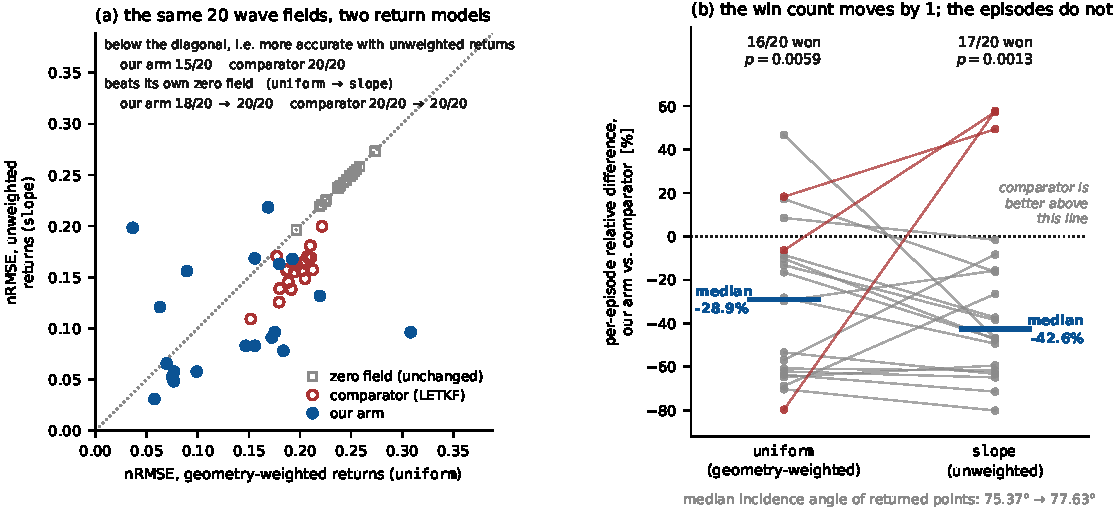
\includegraphics[width=\textwidth]{figures/fig_raydrop.pdf}
\caption{Sensitivity to the spatial weighting of LiDAR returns (B-15). The
simulator can retain a ray hit with a probability weighted by incidence angle and
range, or retain every hit with equal probability calibrated to the same expected
count. The second model's specular gate never fires at this geometry and it always
takes its unweighted path (Section~\ref{sec:experiments}), so this contrast tests
the \emph{weighting} of returns, not diffuse versus specular optics. Both settings
write episode files whose wave fields are identical, so this is a paired
intervention on \BFifteenN{} crowded episodes with no regeneration.
(a)~Per-episode nRMSE under one return model against the same episode under the
other, each point a median over estimator seeds, with each episode's own zero-field
reference. Because the wave field is unchanged that reference is the same on both
axes and lies on the diagonal by construction --- the visual form of the gate that
checked the pairing. \emph{The comparator does not collapse}: it is more accurate
without the weighting on every episode and still beats its own zero field
\BFifteenCmp{}/\BFifteenN{} times there, so the wider margin in panel~(b) is not a
weakened denominator.
(b)~The same comparison as a per-episode relative difference; episodes our arm loses
are drawn in red. Our arm wins \BFifteenBetter{}/\BFifteenN{} without the weighting
($p = \BFifteenP{}$, one-sided sign test, median \BFifteenRel{}). The pre-registered
secondary quantity was the \emph{difference in win counts} between the two settings,
which fell inside the band fixed before the runs; the shift in median size is
descriptive and was not pre-registered. \emph{Read the median as a summary of this
sample, not a per-episode guarantee} --- the per-episode differences move across
most of the plotted range while the win count moves by one.
Three limits travel with it. The ground truth here is linear, because the
higher-order corpus has no counterpart episodes under the second return model, so
this does not stand in for the non-linear result. The intervention is small in what
it changes about the returns --- both median incidence angles are printed on the
figure --- so this is not evidence that a large change would be immaterial. And
\BFifteenRel{} is specific to this sample and this return model: the relative
margins in Table~\ref{tab:earns} are not additive and should not be combined
arithmetically. Crowded stratum only. Generated from the frozen verdict and rows by
\texttt{scripts/gen\_fig\_raydrop.py}, which re-aggregates independently and fails
if the two disagree.}
\label{fig:raydrop}
\end{figure}

\subsection{What carries the gain? Two ablations}
\label{sec:res_ablation}

Baseline comparison alone cannot say \emph{which property} of the estimator is
responsible. We therefore hold the deployed pipeline fixed and remove one property
at a time.

\paragraph{The learned prior}
Replacing the learned set-valued prior with the analytic proposal package, changing
nothing else, removes a margin of \BTwentyTwoRel{} (\BTwentyTwoBetter{}/\BTwentyTwoN{},
$p = \BTwentyTwoP{}$).
\textbf{Disclosure:} the right-hand side of this contrast is \emph{thin, but it has
skill} --- the analytic package beats a zero predictor on
\BTwentyTwoAnaShipZero{}/\BTwentyTwoN{} episodes ($p = \BTwentyTwoAnaShipZeroP{}$),
whereas the learned package does so on \BTwentyTwoLearnZero{}/\BTwentyTwoN{}.
This margin is therefore a comparison between two arms that both work, which is what
makes its magnitude citable at all; the stronger statement --- that the prior is what
makes an arm work \emph{at all} --- belongs to the single-factor swap below, whose
right-hand side does collapse (\BTwentyTwoAnaZero{}/\BTwentyTwoN{}).
$\Rightarrow$ the correct reading is \emph{``the prior is what makes this arm work at all''},
not \emph{``the prior adds a margin on top of a working arm''}.

\paragraph{Continuity of the wavenumber}
% ⛔[2026-09-03 절제 사슬 감사 MAJOR-2] *"leaving every other component untouched"* 는
%   코드상 거짓이다 --- `_snap_k_to_grid` 는 (a)k 반올림 (b)w,φ 전면 재적합
%   (c)옵티마이저 재구성 셋을 한다. ★그러나 `B-20b` 가 재적합 몫을 **직접** 갈랐다.
Snapping atoms to a wavenumber grid removes a margin of \BSixteenRel{}
(\BSixteenBetter{}/\BSixteenN{}, $p = \BSixteenP{}$). Both ablated arms retain skill against a zero field (\BSixteenCmpZero{}/\BSixteenN{} and \BNineteenCmpZero{}/\BNineteenN{}), so the comparator in each case is not empty. The effect is
\emph{dose-responsive}: doubling the grid spacing is worse again
(\BSixteenDose{}/\BSixteenN{}).
% ⛔[2026-09-03 절제 사슬 감사 MAJOR-1] 두 번째 계단의 **우변이 무기술**이다.
%   학위논문은 이미 크기를 철회하고 6/48 을 인쇄한다. 논문은 무공시로 인쇄하고 있었다.
\textbf{Both ablated arms still have skill, which is what makes these comparisons
readable}: on the same episodes the wavenumber-snapped arm beats a per-episode zero
field on \BSixteenCmpZero{}/\BSixteenN{} crowded and \BNineteenCmpZero{}/\BNineteenN{}
sparse episodes, so the comparator we beat was not itself empty.
\textbf{The second rung must be read as a direction, not a size}: the
doubled-spacing arm does not itself beat a zero field, on
\BSixteenDoseCmpZero{}/\BSixteenN{} crowded episodes and on $2/16$ sparse ones, so
the distance between it and the first rung is a distance between a working arm and a
non-working one rather than a performance margin. We therefore report the direction
of the dose--response and not its magnitude. The same ablation reproduces in the sparse stratum
(\BNineteenBetter{}/\BNineteenN{}, \BNineteenRel{}).
\textbf{That operation is not single-factor, and we measured the second factor rather
than assuming it away}: snapping also refits amplitude and phase. A separate batch held
the wavenumbers fixed and applied only the refit; the margin it produced differs from
the one here by $0.23$ percentage points, inside the band that batch fixed in advance,
so the margin is attributable to the quantisation rather than to the refit that
travels with it (B-20b).

\paragraph{What these two magnitudes are not}
They are not additive, and they are not shares of any baseline margin. The reason is
\emph{not} that they come from different corpora --- the two ablations run the same
\AblationEps{} episodes --- but that each removes a different property and is scored
against a different comparison arm, so subtracting one from the other, or from the
baseline margin, has no defined meaning. In particular, the B-1 margin and the
wavenumber-continuity ablation happen to round to the same figure; those two are
measured on different corpora, and the coincidence is arithmetic rather than evidence
that the ablation removes the whole gain.
% ⛔[2026-09-02] 검증 감사 MAJOR: *"Each was measured on **its own corpus**"* 는 **거짓**이다
%   --- `B-16` 과 `B-22` 는 **같은 48 에피소드**다(실측 ∩ = 48/48). 비가법 결론은 옳지만
%   **사유가 틀렸고**, 그 틀린 사유가 「다섯 행이 한 코퍼스의 재채점」이라는 사실을 가렸다.
% ⛔⛔[2026-09-02] **위 주석이 또 본문을 삼켰다**(오늘 세 번째: 국문 초록·영문 초록·여기).
%   ★공시 검사기 `B16-교락폐쇄` 가 잡았다 --- 요구 자구가 사라졌으니 FAIL 이 났다.
%   ⟹ 기계 가드를 신설한다(`check_comment_swallow.py`).
We also checked the grid-snapping ablation separately for
confounding with the amplitude-and-phase refit it necessarily performs, and found the
contribution of that refit negligible.

$\Rightarrow$ Both components that the title names are supported by an intervention
inside our own arm, not only by a comparison against someone else's.

\subsection{Where is the gain? Locating it in space and time}
\label{sec:res_where}

A margin measured on a synthetic corpus can be an artefact of \emph{where} the
corpus places its observations and \emph{when} it scores them. Both coordinates
differ sharply between our synthetic and measured data, so we re-scored the frozen
crowded corpus along each. Both quantities in this subsection are therefore
re-scorings of one corpus --- the same \AblationEps{} episodes that carry the
ablations --- under different questions, not independent experiments, and they use
different comparison arms.

% ============================================================================
% ★2026-09-02 --- 추정 비교를 **그림으로**. 표에만 있고 그림에 없던 둘을 넣는다:
%   (a) 헤드라인의 **짝 구조**(표는 43/48 과 중앙값만 보여 준다)
%   (b) `M-10` 의 **셸 분해 전체**(본문은 한 셸 BAND_REAL 만 인쇄한다)
%   ★(b) 가 이 논문에서 독자가 실제로 묻는 것에 답한다 --- *"센서에서 얼마나 멀리까지"*.
%   ⛔둘 다 제로필드를 **선/점으로** 그린다(F1 부류 차단 --- 서술로만 두지 않는다).
%   ⚠생성기 `scripts/gen_fig_estcompare.py` 는 런 0회이고 동결 verdict 과 재집계가
%     어긋나면 죽는다(근거리 칸을 `verdict_m10.primary.abs_median` 과 대조한다).
% ============================================================================
\begin{figure}[!htbp]
\centering
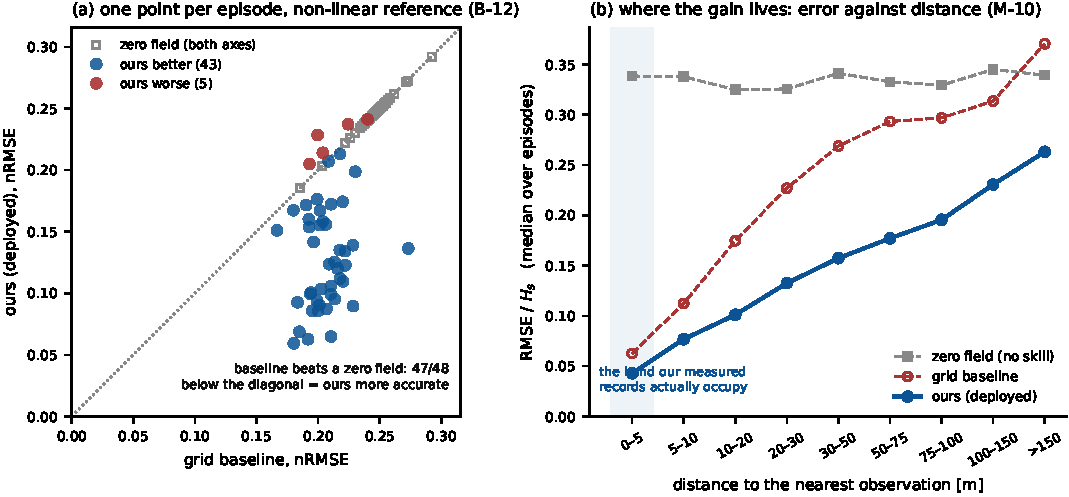
\includegraphics[width=\textwidth]{figures/fig_estcompare.pdf}
\caption{The two comparisons the tables state numerically, drawn.
(a)~Every episode of the non-linear corpus (B-12): our deployed arm against the grid
baseline, one point per episode, each a median over estimator seeds. Points below the
dotted diagonal are episodes we win. The hollow squares are each episode's own
zero-field reference, plotted on both axes, so the reader can see that
\emph{the baseline is not collapsing} --- it beats a zero field on
\BTwelveCmpBetter{}/\BTwelveCmpN{} episodes --- and that the episodes we lose are the
ones where both arms sit close to that reference.
(b)~The same deployed arm scored by distance to the nearest LiDAR observation
(M-10, crowded stratum, $\BOneN{}$-episode corpus). Error grows with distance for
both arms and both approach the zero-field level in the outermost shell: the
representation buys accuracy where there are observations nearby and progressively
less far from them. The shaded shell is the density band our measured records
actually occupy, which is why Section~\ref{sec:res_where} reports that shell rather
than a domain average. \textbf{Disclosures.} M-10 was \emph{not blind} --- its
preregistration recorded the expected direction before the runs, and a smoke subset
had already shown it. The shell boundaries are absolute distances, not multiples of
the peak wavelength, and the corpus mixes two sea states whose peak wavelengths
differ by a factor of $1.65$; \emph{this figure is an exclusion, not an attribution},
and aperture, incidence angle and occlusion remain unmeasured. Both panels are
synthetic and crowded-stratum. Generated from the frozen verdicts and result rows by
\texttt{scripts/gen\_fig\_estcompare.py}, which re-aggregates independently and fails
if the two disagree.}
\label{fig:estcompare}
\end{figure}

\paragraph{Space}
Decomposing the score by distance to the nearest observation, the gain persists
inside the density band that our measured records actually occupy --- points within
$5$~m of an observation --- on \MTenBetter{} of \MTenN{} episodes
(\MTenRel{}), with both arms beating the zero reference there
(\MTenCmp{}/\MTenN{}); Fig.~\ref{fig:estcompare}(b) plots the whole profile.
% [2026-09-02 P9] 4차 감사 B8. ⛔**논문 52쪽에 우리 팔의 절대 정확도가 한 번도 없었다** ---
%   인쇄된 유일한 절대 nRMSE 가 **철회된 기준선의 0.358** 이었다.
%   §4.3 은 "0.10 미만 = excellent" 라는 해석 기준을 주고 값을 한 번도 주지 않는다.
%   값은 `verdict_m10.json` 의 `primary.abs_median` 에 있다(동결).
Because every other number in this paper is a win count or a relative median, we
give the absolute level here as well: on this band the median nRMSE is
\MTenAbsShip{} for the deployed path and \MTenAbsSpec{} for the comparator, against
\MTenAbsZero{} for a zero field. These are medians over the crowded synthetic
stratum and should not be read as a level for any other corpus. This is an \emph{exclusion}, not an attribution: we
did not run an equivalence test, and aperture, incidence angle, and occlusion remain
unmeasured. Not blind.

\paragraph{Time}
The synthetic margins are scored at assimilation time; our measured judgements are
scored at forecast lead. Re-scoring the same frozen corpus at a forecast rung gives
\TFourBetter{}/\TFourN{}, \TFourRel{}.
\textbf{Two disclosures are mandatory here.} First, that rung is at the
\emph{lower} end of the measured lead band: the precise statement is \emph{``a rung
covered by $11$ of the $12$ measured records''}, not \emph{``the same horizon as the
measured data''}. Second, \textbf{the comparator degrades across the same interval}
--- the grid baseline beats the zero reference on \TFourCmpAtZero{}/\TFourN{}
episodes at zero lead but only \TFourCmp{}/\TFourN{} at the reported rung, while our
own absolute error \emph{worsens}. $\Rightarrow$ the growing ratio must not be read as
\emph{``we get relatively better at longer lead''}. Not blind.

% [2026-09-02 P9] 검사기 `크기-결합금지` 가 잡았다: 이 절에 공간.시간 크기가 **나란히**
%   있는데 둘을 비교하지 말라는 문장이 없었다. 두 수는 서로 다른 재채점이다.
The two magnitudes in this subsection answer different questions on different
re-scorings of the same corpus and have no defined meaning relative to each other:
they should not be compared, added, or subtracted, and neither is a decomposition of
any baseline margin.

\subsection{Scope, stated as measured}
\label{sec:res_scope}

\textbf{Against the deployed analytic package, the sparse stratum does not
separate.} With that package's ensemble intact, the learned package wins
\WFifteenCrowdedBetter{}/\WFifteenCrowdedN{} crowded episodes
(\WFifteenCrowdedRel{}\%) but only \WFifteenSparseBetter{}/\WFifteenSparseN{} sparse
ones.\footnote{The crowded count here coincides with the S-ENS crowded count in
Table~\ref{tab:earns}, which is a different contrast on a different corpus
(\SEnsRel{} there against \WFifteenCrowdedRel{} here). Both reproduce from their own
frozen rows; the coincidence is arithmetic.} The win count is not distinguishable from chance; the point estimate
(\WFifteenSparseRel{}\%) is a substantial \emph{loss} and we do not read the null as
equality. We therefore do not write \emph{``the learned prior wins in every
regime''}.
\textbf{The comparator is not weak here, which is what makes this a result.} On the
same episodes the analytic package beats a zero field on
\WFifteenSparseCmpZero{}/\WFifteenSparseN{} sparse episodes, against
\WFifteenCrowdedCmpZero{}/\WFifteenCrowdedN{} in the crowded stratum. The sparse
non-separation is therefore not the artefact this paper warns about elsewhere --- a
margin, or the absence of one, produced by a comparator that had no skill to begin
with. It is the opposite case: the thing we do not beat is the thing that is doing
best.

\textbf{Disclosure:} these figures come from a re-aggregation of the frozen rows
of the deployment-verification batch W-15, not from a pre-registered contrast, and
they do not appear in that batch's verdict file --- the \texttt{sparse} entry there
records a different comparison. Two further caveats travel with them. The zero-field
reference is per-episode and comes from a \emph{different} batch (the same source
W-15's own gate file uses), so the control is assembled across two batches even
though the episode sets are identical. And W-15's corpus is a linear-reference
deployment corpus, not the higher-order corpus of the ablations, so the contrast with
B-19 in the next sentence differs in comparator \emph{and} in corpus.
% ⛔[2026-09-02] 7차 심사 B10·B11: ①제로 기준이 `B_DEPLOY_2026-08-19` 에서 오는데
%   *"On the same episodes"* 만 적고 **배치가 다르다는 것**은 안 적었다(에피소드 집합은
%   동일하지만 W-15 행에는 프레임 수가 없어 정합을 그 행으로는 확인할 수 없다).
%   ②*"one comparator"* 라 적었는데 `B-19` 와는 **코퍼스도 다르다**(선형 vs HOS).
% ⛔[2026-09-02] 검증 감사 MAJOR: 여기 있던 문장은 *"and we cite it as such"* 라 적고
%   **배치 이름도 수치도 인용하지 않았다** --- 게다가 Data availability 는 *"§5 의 모든
%   결과는 배치 식별자를 갖는다"* 는 **전칭**이다. ⟹ 출처를 밝히고 수치를 낸다.
%   재현: `_w15_reagg()` 가 `results.jsonl` 에서 다시 집계한다(혼잡 55/64 · 희소 28/64).
This is a statement about one
comparator on one corpus and does not transfer: against the wavenumber-grid ablation,
on the higher-order corpus, the sparse stratum \emph{does} separate (B-19,
\BNineteenBetter{}/\BNineteenN{}, Section~\ref{sec:res_ablation}). We report both and
collapse neither.

\textbf{On measured data the learned prior does not reach the decision
threshold.} Across $12$
fixed-station stereo records, and under every arm configuration we tested --- including
giving the learned representation the same median-of-$k$ field ensemble that the
deployed real-data path uses --- the learned prior does not reach the pre-registered
threshold against a per-record zero-field reference. The ensemble treatment does move
the endpoint, and it lowers error by a confirmed margin, but it does not cross the
threshold. We report this rather than omit it; a full treatment of the operating
boundary --- including what has been excluded and what remains unmeasured --- is the
subject of a companion thesis. We do not claim to know why the transfer fails.

% ★[2026-09-02] 센서·물리 감사의 신규 소견. 이 문단이 지는 비교(팔 대 참 제로필드)가
%   바로 편향된 형태다 ⟹ 본문이 그것을 적는다(그림 캡션만으로는 부족하다).
\textbf{One asymmetry runs through every measured comparison of this form.} The window
the estimator observes and the window it is scored on are de-meaned separately, per
pixel, which leaves a static spatial offset between them worth $0.05$--$0.29$ of the
record's standard deviation. A fitted wave field is a sum of travelling components and
cannot represent a static pattern, so that offset is an irreducible error floor for any
arm that fits; the zero-field reference, being identically zero, does not carry it. Every
\emph{arm-versus-zero} statement about the measured records is therefore biased against
the arm. This does not weaken the negative --- it means the negative is partly a property
of the scoring convention, and that a positive obtained under it is conservative. The
\emph{paired} comparisons between arms are unaffected, because both arms are fitted to
the same observations and inherit the same offset.

% ★[2026-09-02] `R1b` — 위 문단이 서술한 결함을 **고쳐서 다시 채점한 결과**.
%   ⛔이 배치는 규약을 **채택하지 않는다**(배포 기본값 불변). 답한 질문은 하나:
%   *"고치면 판정이 바뀌는가"*. ⛔`Old` 계수를 `B-2` 공표값과 직접 비교 금지 --- 그쪽은
%   수심 정정 **전**(17 m)이고 여기는 후(30 m)다. 동결 = `verdict_r1b.json`.
\textbf{We repaired that convention and re-scored; the verdict holds.} The repair
de-means the scored window with the observation window's own per-pixel mean. It was
chosen before any arm score was computed, on two criteria that depend only on the
definition of the ground truth: the true field must score zero, and the lead-zero
target must not depend on how far ahead a batch chose to score. Under it the deployed
arm beats the per-record zero field on \ROneBShipFixed{}/\ROneBN{} records
($p = \ROneBP{}$), against \ROneBShipOld{}/\ROneBN{} under the biased convention;
the learned representation moves from \ROneBPropOld{}/\ROneBN{} to
\ROneBPropFixed{}/\ROneBN{} and still does not reach the pre-registered threshold of
ten.
% ★[2026-09-03] N−1 방지: §Limitations 에 R8 을 실었는데 **이 숫자가 나오는 자리**에
%   상호참조가 없으면 독자는 지지집합 조건 없이 11/12 를 읽는다.
The deployed arm's \ROneBShipFixed{}/\ROneBN{} should be read with the support condition
below: on these records the query points sit a few hundredths of a wavelength from the
nearest observation, and when the observations are confined to half the box the same
arm keeps skill on only \REightSkillOut{}/\REightN{} of them --- though that reduction
does not reproduce in the stratum with the most query points (\REightBigW{} of
\REightBigN{}), so we state both. The repair is not a favourable one. The median comparator shift is
\ROneBZeroMed{}; eleven of twelve records move by less than three percent in either
direction; and on four of them the comparator becomes \emph{stronger}, which makes it
harder to beat. One record carries the whole change (\ROneBZeroMax{}), and it is the
same record whose lead-zero target is most sensitive to the scoring-window length ---
the two defects are largest in the same place. The repaired scoring is not blind: the
counts under the biased convention were known when the batch was frozen, and the
design cannot reach a confirmatory grade under its own stated prediction, so we report
it as exploratory.

% ★★[2026-09-03] `E1-EXTBASE`. 이 원고와 학위논문이 *"실측 외부 기준선 행 0개"* 를
%   여러 곳에 인쇄하고 있었는데 **오늘 그것이 거짓이 됐다**. ⛔예산 규약 병기 의무.
\paragraph{An external baseline, and it does not flatter us}
Until today this paper reported no external baseline on the measured records, and
recorded that absence as a measured state: two attempts failed their own self-test.
That is no longer the situation. We ran a third-party reconstructor --- published code
under GPL-3 with the authors' own pre-trained weights, neither their code nor ours
modified --- on the same twelve records, and swept the observation budget.

The robust result is the ladder rather than the contest. At the density our deployment
geometry actually supplies, twelve points per frame, that method clears a per-record
zero field on \EOneSelfTwelve{}/\EOneN{} records; at two hundred points per frame it
clears on \EOneSelfTwoHundred{}/\EOneN{}, and at four hundred on
\EOneSelfFourHundred{}/\EOneN{}. \emph{The budget at which an external reconstructor
begins to have skill on these records lies between two and four hundred points per
frame, and our sensing geometry delivers twelve.} That converts a limitation this paper
previously asserted into one it measures.

The head-to-head must be read with the budget convention attached, because the two
methods consume observations differently: our arm accumulates twelve points per frame
over a forty-second memory window, while theirs sees three consecutive frames and
cannot use a history. At \emph{equal total budget} --- six hundred observations each ---
the deployed arm is better on \EOneEqualShipWin{}/\EOneEqualN{} records, which is a tie,
and at that budget the external method does not reliably clear a zero field
(\EOneSelfTwoHundred{}/\EOneN{}). At the lowest budget where it does clear, it is
receiving twice our observations, and there it beats the deployed arm on
$\EOneN{}-\EOneShipWin{}$ of \EOneN{} records ($p = \EOneP{}$). Our arm beats a
per-record zero field on eleven of twelve throughout. Three further conditions travel
with the comparison: their input spans $t-1,t,t+1$ and therefore sees a future frame,
which favours them; their dense output is resampled onto our query grid by nearest
neighbour; and the training distribution of their checkpoint could not be read from the
publisher, so its relation to these sites is unknown.

% ⛔[2026-09-02] 적대적 감사 M3·M4. 두 공시 없이 위 문단의 p 를 인쇄하면 독자가
%   *"수리가 실측 헤드라인을 유의하게 만들었다"* 로 읽는다. 둘 다 거짓이 아니라 **미공시**였다.
\textbf{Two things must be read with that $p$-value.} First, this arc records a
sixteen-arm Holm family whose smallest threshold is $0.05/16 = 0.0031$; the repaired
$p$ moves the deployed arm from $0.0193$ to $\ROneBP{}$ and still does not cross it, so
the statement that no arm on the measured records survives the multiplicity correction
is unchanged. Second, the sign test treats the twelve records as independent, and they
are not: they come from four sites and ten calendar days, with three records drawn from
a single afternoon. Folded to days the count is $9/10$ ($p = 0.011$); folded to sites it
is $4/4$, whose $p$ is $0.0625$ --- the floor, so at site level $\alpha = 0.05$ is
unreachable by construction. The result survives the day-level fold and we report the
record-level number as the pre-registered one, not as the strongest one.

% ★[2026-09-02] 문헌 실사 E. ⛔이 문단은 **변호가 아니라 위치지음**이다 --- 우리 관행이
%   관례 안이라는 것과, 관례 자체의 상한이 어디인지를 함께 적는다.
%   확인 수준: Wang 2025 · Desmars 2023 · Wang&Pan 2021 은 **원문 전문**,
%   WASS/Benetazzo 계열은 2차 서술(Guimarães 2020 원문의 인용 포함).
\textbf{This construction is the field's, not ours alone.} Validation practice in
phase-resolved wave reconstruction spans a narrow spectrum: purely synthetic references;
wave-tank experiments whose dense truth is assembled by exploiting repeatability across
runs~\citep{desmars2020}; field campaigns scored against the same sensor's later frames
because a true solution is unavailable; and field observations checked against
independent \emph{point} sensors at the level of spectra and scalar statistics. A dense,
field-scale reference that is independent of the observing sensor does not, to our
knowledge, exist anywhere in this literature --- even the stereo surfaces used as ground
truth trace their own validation to centimetre-level comparisons against point gauges.
% ★[2026-09-02] `R2b` --- 위 문장이 서술하는 *"점 게이지 대조"* 를 **우리가 직접 했다**.
%   ⛔면 참값 주장 아님 · ⛔격자점별 오차장 주장 아님(6점, 반경 0.25 m, 격자에서 7--11 m).
%   동결 = tmp/R2B_STEREONOISE_2026-09-02/verdict_r2b.json (게이트 13/13)
\textbf{We ran that point comparison ourselves and report the number.} On the seven
records for which a co-located wave-gauge array exists, the stereo surface carries more
variance above $1$~Hz than the gauges do on \RTwoBBetter{}/\RTwoBN{} records
($p = \RTwoBP{}$), by \RTwoBFloorMin{}--\RTwoBFloorMax{}~mm RMS (median
\RTwoBFloorMed{}~mm). That is an \emph{upper} bound on the reconstruction noise floor:
the gauges carry their own noise, and they sample a different point of a spatially
inhomogeneous field. It does not make the surfaces a validated dense reference --- the
gauges are six sensors within a $0.25$~m radius, $7$--$11$~m from the scored grid, so no
per-gridpoint error field follows. Two conditions travel with the number: the comparison
rests on the gauges being far enough from the scored grid that no positional
correspondence is usable, and \emph{that} premise is asserted here rather than
established: the search we ran to test it swept lags of $\pm 20$~s while the two
instruments' record clocks are offset by $400$--$1046$~s, so it never visited the true
alignment. A re-check at the true offset leaves the conclusion standing but the
pre-registered evidence for it does not. The surrogate null we used is justified by the
gauge series being near-Gaussian, which holds on four of the seven.
The closest competing study evaluates on one of the same public stereo records we use,
takes that dense reconstruction as its ground truth, and additionally subsamples it
synthetically~\citep{Wang2025PointsToWaves}. What is specific to us is one further
synthetic layer: our sparse pattern follows a simulated scanning-LiDAR geometry rather
than the sparse output of a real stereo matcher, and our records come from fixed stations
rather than a vessel. We state that asymmetry rather than let the shared convention
excuse it.

% ★[2026-09-02] 실측 그림 신설. 사용자 요청(*"실측 데이터랑도 뽑아줘"*).
%   ⛔런 0회 --- 동결 행 재집계. 생성 = scripts/gen_fig_real.py (방벽이 재생성 대조한다).
%   ⛔캡션에 계수를 손으로 적지 않는다. 그림이 그 수를 진다.
\begin{figure}[!htbp]
\centering
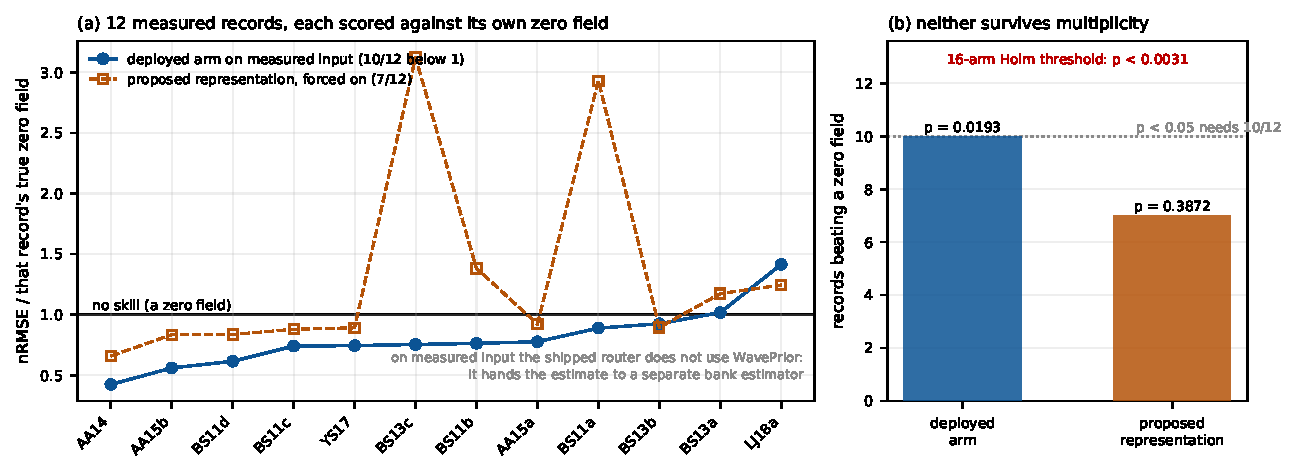
\includegraphics[width=\textwidth]{figures/fig_real.pdf}
\caption{The measured records, scored the way the correction of the scoring
reference requires. Each of the $12$ fixed-station stereo records is divided by
\emph{its own} true zero-field error rather than by a constant: that constant was
found to be wrong, and the per-record values span more than a factor of three, so a
single reference silently rescales the records against one another. A value of $1$ is
the error of predicting a flat sea. Panel (b) counts the records each arm places
below that line and marks the threshold that the multiplicity correction for this
arc imposes; the deployed arm reaches ordinary significance and neither arm reaches
the corrected threshold, which is why the text reports no skill rather than a small
one. Two things must be read with the figure. First, the arms are drawn at the
corrected water depth, taken from the batches that already contain that
configuration; the records the correction cannot touch are bit-identical between the
two depths, which is what makes the pairing legitimate. Second, and more important
for this paper's title: \emph{on measured input the shipped router does not use the
learned prior at all} --- it hands the estimate to a separate bank estimator, and the
``proposed representation'' arm is that prior switched on by force. The two arms are
each scored against their own zero-field reference and are not compared to one
another here, because the paired margin between them has been corrected twice and is
not a quantity this paper cites. \emph{One asymmetry must be read with the counts.} The
observation window and the scoring window are de-meaned separately, per pixel, so a static
spatial offset of $0.05$--$0.29$ of the record's standard deviation stands between them. A
fitting arm cannot represent that offset and carries it as an error floor; a zero
predictor, which predicts nothing, does not. Both counts are therefore biased
\emph{against} the arms: what survives is conservative, and a reading of ``no skill'' is
helped by the artefact rather than hindered by it; on the single record where that floor
is largest it accounts for most of the scoring reference, and that record is also the one
counterexample in the paired comparison, so we do not build any statement on it alone.
Section~\ref{sec:res_scope} reports the same counts under a repaired convention, where
each arm gains exactly that one record and the learned arm still falls short.
\emph{Three further conditions.} The scored points are a $4$~m subsample of the same grid
the observations are drawn from, but no scored value was ever handed over as an
observation, and a nearest-neighbour interpolator using that proximity clears the
zero-field reference on none of the records --- what is scored is a space-time model, not
an interpolation. The scored instant is the right-hand endpoint of the observation
window, so this figure is a reconstruction, \emph{not} a forecast. And the multiplicity
threshold drawn in panel~(b) counts sixteen arms, of which six are bit-identical
repetitions; on the ten distinct hypotheses the threshold is looser, and neither arm
crosses it either way.}
\label{fig:real}
\end{figure}

% ★[2026-09-02] 실측 정성 그림. ⚠생성기는 **추정을 2회 돌린다**(레코드 1 × 팔 2)
%   ⟹ ⛔방벽의 「재생성 대조」 목록에 넣지 않는다(방벽은 런 0회여야 한다).
%   대신 생성기 자신이 동결 행과 **비트 대조**한다: obs/q 해시 · 두 팔의 nowcast ·
%   원자 수 · 참 제로필드. 불일치면 그림을 저장하지 않고 죽는다.
\begin{figure}[!htbp]
\centering
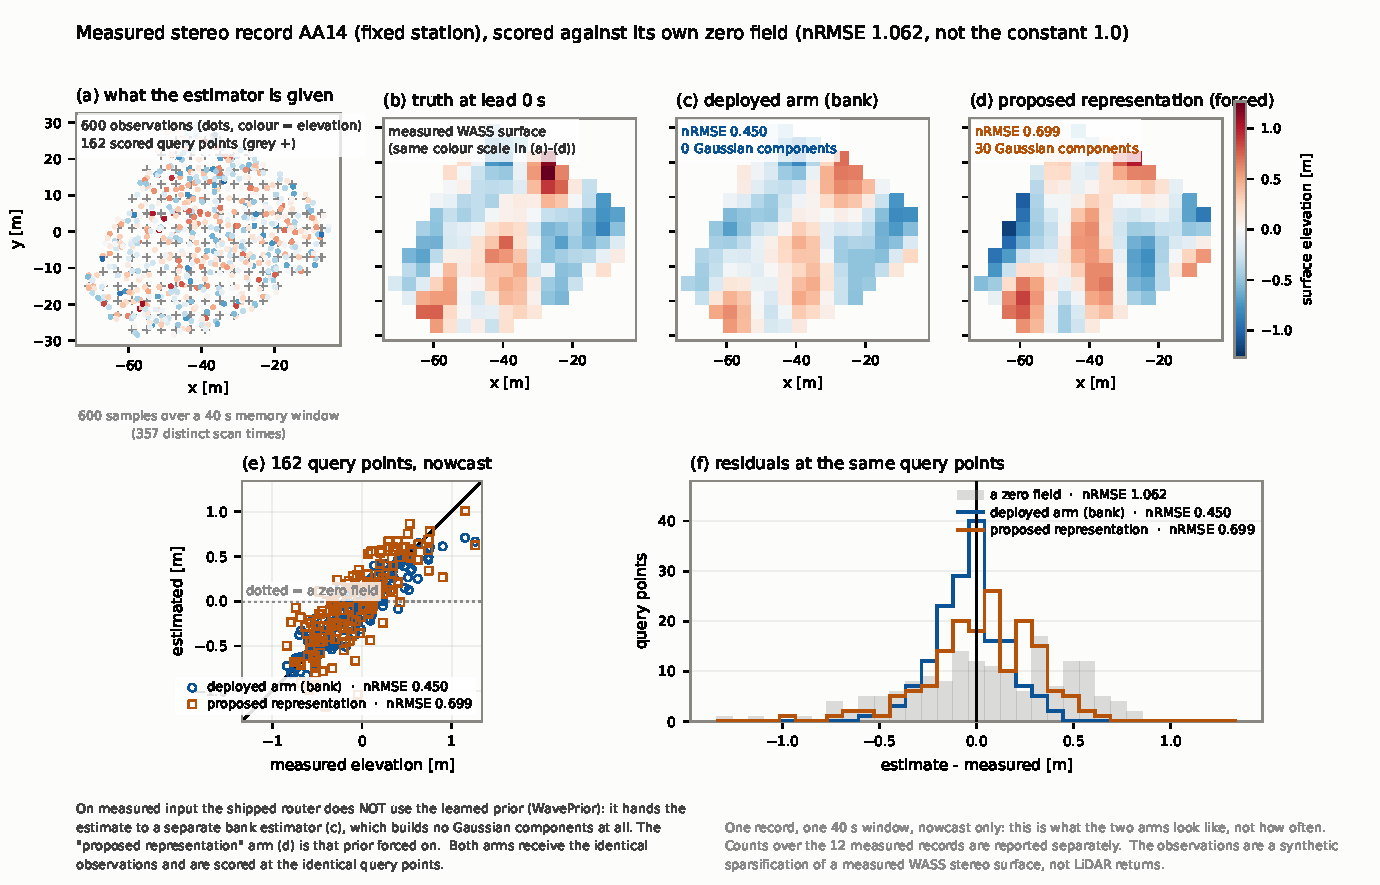
\includegraphics[width=\textwidth]{figures/fig_real_qual.pdf}
\caption{What the two arms actually produce on one measured record, so that the
counts in Fig.~\ref{fig:real} have a picture attached. Both arms receive the
identical observations (a) --- a sparse sample of a measured stereo surface, not
lidar returns --- and are scored at the identical query points against the measured
surface (b). The deployed arm (c) builds no spectral components at all: on measured
input the shipped router does not use the learned prior, and hands the estimate to a
separate bank estimator. Panel (d) is that prior switched on by force. Panels (e) and
(f) show the same two estimates at the query points, with a zero field drawn as the
reference each is scored against. \emph{This is one record, one window, and the
nowcast only:} it shows what the arms look like, not how often. The record was chosen
because the water-depth correction does not touch it, which is what allows the
figure's numbers to be checked bit-for-bit against the frozen batch; it also sits in
the easier of the two spatial strata. The ratio of the two errors here is not a
result --- the paired margin between these arms has been corrected twice and is not a
quantity this paper cites.}
\label{fig:real_qual}
\end{figure}


\subsection{Summary of the measurements this paper rests on}
\label{sec:res_summary}

% ============================================================================
% ★2026-09-02 (P9) --- 표.그림 처분.
%   이 자리에 있던 세 절(Ablation study / Raydrop model sensitivity /
%   Robustness: sparsity, noise, and sea state)과 그 표 넷.그림 넷은
%   **철회된 코퍼스**(두 팔이 같은 프레임에서 채점된 적이 없는 100ep 코퍼스, 그리고
%   추적기 위상전개 수정 **이전**의 실행) 산물이다.
%   ⟹ tmp/PAPER_LEGACY_2026-09-01/retracted_tables_2026-09-02.tex 로 **옮겼다**(삭제 아님).
%   그 자리에 들어가는 아래 두 표는 **전부 사전등록.동결된 verdict_*.json 원자**이고
%   paper_constants.tex 를 거친다 --- 손으로 적힌 수가 한 개도 없다.
%   ⚠이 처분은 논문을 **얇게** 만든다. 그것을 본문에서 **말한다**(아래 마지막 문단).
% ============================================================================

Table~\ref{tab:earns} and Table~\ref{tab:boundary} collect every comparison this
paper relies on for its accuracy claims, and Fig.~\ref{fig:results} plots the first
of them with exact confidence intervals alongside each comparator's own skill. Three
contrasts are reported outside them and are marked where they appear: the
spectral-domain measurement of Section~\ref{sec:res_spectral}, which is graded
exploratory; the ensemble contrast on measured records later in this section, which
moves an endpoint without crossing a threshold; and the sparse-stratum figure in
Section~\ref{sec:res_scope}, which is a re-aggregation of a frozen deployment
corpus rather than a pre-registered contrast.
% ⛔[2026-09-02] 검증 감사 MAJOR: *"Two contrasts"* 도 여전히 **부족**했다 --- 초록이 기대는
%   §5.6 의 희소 재집계가 셋째다. ★전칭을 좁힐 때 **한 칸만 좁히면 다시 틀린다**.
% ⛔[2026-09-02] 6차 감사 N13: *"collect **every** comparison"* 은 **전칭이고 거짓**이었다.
%   ★전칭을 쓸 때마다 이 저장소가 대가를 치렀다(오늘 두 번째).
 Each row is one batch, and the number is read out of that batch's
frozen verdict file rather than transcribed by hand.
% ============================================================================
% ★2026-09-02 (P9) --- 내 전칭 주장 수리. 초판(오늘 아침)은 *"Each row is one
%   pre-registered batch: … the analysis code was frozen by checksum"* 라 적었다.
%   ⛔**B-1 에는 거짓이다** --- `verdict_b1.json` 의 `_honesty` 축자:
%   *"gates_b1.py / analyze_b1.py 는 결과 뒤에 작성됐다(2026-08-23)."*
%   ★항진 검사가 「발동하지 않는 규칙」을 보고해서 찾았다(규칙 트리거가 좁았다).
% ============================================================================
For all but one, the decision rule, the comparison, and the reading were fixed in a
preregistration before the runs produced a single result row, and the analysis code
was frozen by checksum. The exception is the B-1 row: its gate and analysis scripts
were written after the results existed, transcribing rules that had already been
recorded in the batch's design note. We state this rather than let the word
``pre-registered'' cover it.
Table~\ref{tab:earns} is what the representation earns on synthetic corpora,
where ground truth exists; Table~\ref{tab:boundary} is where it stops, on the
$12$ measured records. Fig.~\ref{fig:qualitative} shows one reconstruction in full, as an
illustration rather than as evidence.

% [2026-09-02 P9] 4차 감사 B7 후속: `table*` 은 별표 float 이라 `[h]`/`[b]` 가 없다
%   ⟹ 한 번 못 앉으면 **문서 끝까지 밀린다**(표 5 가 참고문헌 뒤로 갔다).
%   review 모드는 단일단이라 별표가 필요 없다 ⟹ 보통 table 로 내린다.
\begin{table}[!htbp]
\centering
\caption{What the representation earns. All contrasts are paired per episode and
one-sided in the pre-registered direction; ``better'' counts episodes on which the
first arm has lower nRMSE, and the relative median is the median of the paired
relative differences. Crowded stratum unless noted. \emph{Read the third column
with the fourth}: a large margin against a comparator that itself has little skill
is not the same measurement as a large margin against one that does, which is why
the ``cmp.'' column is printed rather than described: it counts the episodes on
which the \emph{comparator} beats a zero predictor, i.e.\ how much skill the thing
we beat had. A dash means the batch did not carry that control; where the value
exists it is printed, and the two representation rows carry theirs with a
qualification given below. A dash in the
$p$ column means the batch's decision rule is not a single sign test on this
contrast (B-26 reads a $2\times2$ design, T-4 a lead ladder, and the sparse S-ENS row
is undecided).
These rows are separate
\emph{contrasts}, not separate corpora --- \HosSameN{} of them re-score the same
\AblationEps{} episodes under different arms (note~(i)) --- and their magnitudes have
no defined meaning when added or subtracted.}
\label{tab:earns}
% [2026-09-02 P9] 4차 감사 M4: 이 tabular 가 본문 폭을 81.9pt(약 2.9 cm) 넘었다.
%   `[review]` 의 넉넉한 여백 때문에 눈에 안 띄었을 뿐, 저널 판형에서는 잘린다.
\footnotesize
\setlength{\tabcolsep}{4pt}
\begin{tabular}{llccrrc}
\toprule
Question & Batch & $n$ & better & rel.\ median & $p$ & cmp. \\
\midrule
\multicolumn{7}{l}{\emph{Against an external baseline}} \\
Strongest eligible baseline & B-1  & \BOneN{}    & \BOneBetter{}    & \BOneRel{}    & $\BOneP{}$ & (\BOneCmp{}/\BOneCmpN{}) \\
Non-linear ref., \BTwelveFreshSeeds{}/\BTwelveSeeds{} new seeds & B-12 & \BTwelveN{} & \BTwelveBetter{} & \BTwelveRel{} & $\BTwelveP{}$ & \BTwelveCmpBetter{}/\BTwelveCmpN{} \\
Unweighted sensor returns & B-15 & \BFifteenN{} & \BFifteenBetter{} & \BFifteenRel{} & $\BFifteenP{}$ & \BFifteenCmp{}/\BFifteenN{} \\
Sea state matched to records & B-26 & \BTwentySixN{} & \BTwentySixBetter{} & \BTwentySixRel{} & --- & \BTwentySixCmpBetter{}/\BTwentySixN{} \\
\midrule
\multicolumn{7}{l}{\emph{Ablations of the representation itself}} \\
Continuity of the wavenumber & B-16 & \BSixteenN{} & \BSixteenBetter{} & \BSixteenRel{} & $\BSixteenP{}$ & \BSixteenCmpZero{}/\BSixteenN{}$^\dagger$ \\
\quad --- sparse stratum & B-19 & \BNineteenN{} & \BNineteenBetter{} & \BNineteenRel{} & $\BNineteenP{}$ & \BNineteenCmpZero{}/\BNineteenN{} \\
The learned prior & B-22 & \BTwentyTwoN{} & \BTwentyTwoBetter{} & \BTwentyTwoRel{} & $\BTwentyTwoP{}$ & \BTwentyTwoAnaShipZero{}/\BTwentyTwoN{} \\
Ensemble on learned path & S-ENS & \SEnsN{} & \SEnsBetter{} & \SEnsRel{} & $\SEnsP{}$ & --- \\
\quad --- sparse stratum & S-ENS & \SEnsSparseN{} & \SEnsSparseBetter{} & \emph{undecided} & --- & --- \\
\midrule
\multicolumn{7}{l}{\emph{Where the gain sits}} \\
In space (inside observed band) & M-10 & \MTenN{} & \MTenBetter{} & \MTenRel{} & $\MTenP{}$ & \MTenCmp{}/\MTenN{} \\
In time (lead $1.0\,T_p$) & T-4 & \TFourN{} & \TFourBetter{} & \TFourRel{} & --- & \TFourCmp{}/\TFourN{} \\
\bottomrule
\end{tabular}

{\footnotesize $^\dagger$Measured by re-aggregating that batch's frozen rows against a
per-episode zero field on 2026-08-27; it was not a pre-registered contrast of B-16. The
sparse row's value \emph{was} a named gate of B-19.\par}

\end{table}

% ============================================================================
% ★2026-09-02 (P10) --- 5차 감사 도전 E / 권고 3b:
%   *"No absolute-error table … this venue expects nRMSE **and** RMSE in metres,
%    by stratum, with dispersion."*
%   ⛔런 0회다: 합성 하네스가 `nRMSE = RMSE / Hs` 로 정규화하므로
%   (`metrics.py:32-50`) 미터는 **정의에서** 나온다. 새 측정이 아니다.
%   ★생성기가 교차 검증을 한다: 같은 팔이 두 배치에서 값이 다르면 죽는다.
% ⛔[2026-09-02] 6차 감사 N: 이 표를 **본문이 한 번도 인용하지 않았다**
%   (`\ref{tab:absolute}` 0회) --- 5차 감사가 지적한 바로 그 결함을 새 표가 재현했다.
% ============================================================================
\paragraph{The same numbers in metres}
Every quantity above is a ratio. Table~\ref{tab:absolute} restates in metres, by sea
state and with interquartile ranges, the arms of the non-linear replication (B-12)
and of the three ablations that carry the paper's claims --- wavenumber continuity in
both strata (B-16, B-19) and the learned prior (B-22).
% ⛔[2026-09-02] 7차 심사 B8: 이 문장이 *"the three **ablation** batches"* 라 적었는데
%   `B-12` 는 절제가 아니라 기준선 대비 행이고, **논문의 중심 절제 `B-22` 는 표에
%   아예 없었다** --- 독자가 해석적 패키지의 절대 수준을 볼 수 없었다.
It is a
unit conversion and not a new measurement --- the synthetic harness normalises by
significant wave height, so metres follow by multiplication --- but it is the form
in which a reader can ask whether the residual is small compared with the sea it
sits in. Two things are visible there that a ratio hides. The crowded-stratum error
of the deployed arm is roughly a seventh of the wave height at BF4 and an eighth at
BF5, while its comparator sits near a fifth in both. And the sparse block's large
relative margin survives the conversion --- it is not an artefact of dividing by a
small number --- but its absolute errors are also the smallest in the table, so the
margin is measured where there is least to get wrong. That is a different fact from
the one in Section~\ref{sec:res_scope}, which reports that the sparse stratum does
not separate against a \emph{different} comparator, the deployed analytic package;
the two are not in conflict and neither generalises to the other.

% ⛔자동 생성 — 손으로 고치지 마라.
%    생성: python3 scripts/gen_abs_table.py   (런 0회, 동결 행 재집계)
%    변환: RMSE[m] = nRMSE x Hs  (metrics.py:32-50)

\begin{table}[!htbp]
\centering
\footnotesize
\caption{Absolute accuracy, in the units the measurement is made in and in metres. The synthetic harness normalises by significant wave height, so metres follow from $\text{RMSE} = \text{nRMSE}\times H_s$ with no new measurement; this table is a re-aggregation of the same frozen rows that produce Table~\ref{tab:earns}. Each cell is the median over episodes of the per-episode median over estimator seeds, with the interquartile range. \emph{Read within a sea state, not across:} $H_s$ differs between the two, so the ordering in metres and the ordering in nRMSE need not agree across rows. B-12 and B-16 score their arms on the same \AblationEps{}-episode corpus, so their \texttt{SHIP-NOW} cell is one cell, not two; it is listed once, under B-12, and the generator cross-checks the two aggregations and fails if they disagree.}
\label{tab:absolute}
\setlength{\tabcolsep}{4pt}
\begin{tabular}{lcrrrr}
\toprule
Arm & sea state & $H_s$ [m] & $n$ & nRMSE & RMSE [m] \\
\midrule
\multicolumn{6}{l}{\emph{B-12  non-linear ref.\ (crowded)}} \\
\quad \texttt{SHIP-NOW} & BF4 & 1.2 & 24 & 0.137 {\scriptsize[0.096,0.203]} & 0.164 {\scriptsize[0.115,0.244]} \\
\quad \texttt{SHIP-NOW} & BF5 & 2.0 & 24 & 0.130 {\scriptsize[0.096,0.158]} & 0.259 {\scriptsize[0.191,0.315]} \\
\quad \texttt{SPEC25} & BF4 & 1.2 & 24 & 0.209 {\scriptsize[0.201,0.218]} & 0.251 {\scriptsize[0.241,0.261]} \\
\quad \texttt{SPEC25} & BF5 & 2.0 & 24 & 0.199 {\scriptsize[0.191,0.213]} & 0.399 {\scriptsize[0.381,0.425]} \\
\midrule
\multicolumn{6}{l}{\emph{B-16  $k$ ablation (crowded)}} \\
\quad \texttt{KGRID1} & BF4 & 1.2 & 24 & 0.228 {\scriptsize[0.202,0.244]} & 0.273 {\scriptsize[0.243,0.292]} \\
\quad \texttt{KGRID1} & BF5 & 2.0 & 24 & 0.204 {\scriptsize[0.176,0.228]} & 0.408 {\scriptsize[0.353,0.457]} \\
\quad \texttt{KGRID2} & BF4 & 1.2 & 24 & 0.302 {\scriptsize[0.278,0.316]} & 0.363 {\scriptsize[0.334,0.379]} \\
\quad \texttt{KGRID2} & BF5 & 2.0 & 24 & 0.278 {\scriptsize[0.247,0.318]} & 0.556 {\scriptsize[0.494,0.635]} \\
\midrule
\multicolumn{6}{l}{\emph{B-19  $k$ ablation (sparse)}} \\
\quad \texttt{KGRID1} & BF4 & 1.2 & 8 & 0.216 {\scriptsize[0.186,0.275]} & 0.259 {\scriptsize[0.223,0.331]} \\
\quad \texttt{KGRID1} & BF5 & 2.0 & 8 & 0.221 {\scriptsize[0.193,0.254]} & 0.441 {\scriptsize[0.387,0.507]} \\
\quad \texttt{KGRID2} & BF4 & 1.2 & 8 & 0.340 {\scriptsize[0.271,0.360]} & 0.408 {\scriptsize[0.325,0.432]} \\
\quad \texttt{KGRID2} & BF5 & 2.0 & 8 & 0.297 {\scriptsize[0.270,0.332]} & 0.593 {\scriptsize[0.539,0.663]} \\
\quad \texttt{SHIP-NOW} & BF4 & 1.2 & 8 & 0.053 {\scriptsize[0.022,0.070]} & 0.063 {\scriptsize[0.026,0.084]} \\
\quad \texttt{SHIP-NOW} & BF5 & 2.0 & 8 & 0.083 {\scriptsize[0.039,0.204]} & 0.166 {\scriptsize[0.078,0.408]} \\
\bottomrule
\end{tabular}
\end{table}


\paragraph{What each $n$ is made of, and why it is not $n$ independent trials}
% ============================================================================
% ★2026-09-02 (P10) --- 5차 감사 도전 B·F. 두 지적이 한 문단으로 답해진다:
%   B *"64 'episodes' … the sign test treats them as 64 i.i.d. trials"*
%   F *"corpus composition is never given"*
%   ⛔수는 손으로 적지 않는다: 동결 `results.jsonl` 에서 센다(`gen_paper_constants.py`).
% ============================================================================
The episode counts in Table~\ref{tab:earns} are not independent draws, and we state
% ⛔[2026-09-02] 초록 헤드라인이 `B-12`(48 에피소드)로 바뀐 뒤 이 문장의
%   *"headline corpus of 64"* 가 **초록과 충돌**한다(검증 감사). 배치 이름으로 바꾼다.
what they are. The B-1 corpus of \HeadlineEps{} crowded episodes is a full
factorial: \HeadlineSeeds{} generator seeds crossed with two Beaufort levels and two
component counts. The \AblationEps{}-episode corpus used by the ablations and by the
non-linear replication is the same design with \AblationSeeds{} seeds. So four
episodes share each seed, and the true number of independent scene draws behind an
$n$ of \AblationEps{} is \AblationSeeds{}, not \AblationEps{}.

A second axis is folded away before the sign test sees it. Each episode is run at
\EstSeeds{} estimator seeds and the value entering a comparison is the median over
them, so estimator-side randomness is suppressed rather than counted; the S-ENS rows
are the exception and use \EstSeedsSEns{}, which that batch discloses. This makes the
comparisons more stable but it does not add independent trials.

The sign tests we report treat episodes as exchangeable. That is the convention the
preregistrations fixed, and we keep it rather than change the rule after the fact,
but it means the $p$-values should be read as descriptive of the paired pattern
rather than as calibrated tail probabilities: if the seed is the dominant source of
scene-to-scene variation, the effective sample size lies somewhere between
\AblationSeeds{} and \AblationEps{}, and every $p$ we print is correspondingly
optimistic. No result in this paper turns on a marginal $p$ --- the confirmatory
rows clear their thresholds by several episodes --- but a reader comparing two of
them on the strength of $p$ alone would be over-reading.

\emph{We therefore also report the load-bearing rows under the most conservative
convention available}: fold each scene seed's episodes to their median, and sign-test
on \emph{seeds}. This floors $p$ at $2^{-n}$ and it is a re-aggregation of the frozen
rows rather than a pre-registered contrast, but it removes the objection entirely.
B-1 gives \BOneSeedW{}/\BOneSeedN{} ($p = \BOneSeedP{}$), B-12
\BTwelveSeedW{}/\BTwelveSeedN{} ($p = \BTwelveSeedP{}$), B-16
\BSixteenSeedW{}/\BSixteenSeedN{} ($p = \BSixteenSeedP{}$) and B-22
\BTwentyTwoSeedW{}/\BTwentyTwoSeedN{} ($p = \BTwentyTwoSeedP{}$). Every one still
clears $\alpha/2 = 0.025$, so the conclusions do not rest on treating episodes as
independent. \emph{The $p$ column of Table~\ref{tab:earns} is the episode-level
value} and should be read with this paragraph.
% ★[2026-09-02] 7차 심사 B14: 심사자 축자 --- *"A referee cannot let a table assert what
%   the surrounding text says is wrong."* 이 문단이 *"인쇄된 모든 p 는 그만큼 낙관적"*
%   이라 적으면서 표는 1.13e-16 을 싣고 있었다. ⟹ **가장 보수적인 규약으로 다시 집계**해
%   같이 싣는다. ★결과가 주장을 지탱한다(전건 α/2 통과) --- 숨길 이유가 없었다.

\paragraph{How the rows of Table~\ref{tab:earns} must be read}
Four qualifications apply to the table as a whole and are not repeatable per row.
\emph{(i)} Every corpus in it is synthetic, and the rows are less independent of one
another than a table of separate batch identifiers suggests. Six of them
(\HosRows{}) draw on the higher-order (HOS) reference corpus, and \HosSameN{} of
those (\HosSameRows{}) run the \emph{identical} \AblationEps{} episodes --- they are
re-scorings of one corpus under different arms, not independent experiments.
\HosDisjointRows{} uses a disjoint \BNineteenN{}-episode subset of the same
directory. The remaining \LinearN{} batches (\LinearRows{}) use a linear ground-truth
field; S-ENS occupies two of the table's rows.
% ⛔[2026-09-02] 검증 감사 BLOCKER: 이 자리에 있던 *"세 행이 HOS 를 공유"* 는 **틀렸다**
%   --- `B-22`·`M-10`·`T-4` 도 `gates_b11.HOS` 를 임포트한다(파일:줄 = `gates_b22.py:70` ·
%   `gates_m10.py:50` · `gates_t4.py:50`). 실측 교집합: 다섯 행이 **48/48 동일**.
%   ★그래서 이제 이 문장의 수치는 `_corpus_identity()` 가 **행에서 센다** --- 다음 배치가
%   같은 코퍼스를 쓰면 매크로가 저절로 따라간다.
% ⛔[2026-09-02] **주석이 본문을 삼켰다** — 아래 한 줄이 그 복구분이다.
``Higher-order'' names what was \emph{requested} of the
generator, not what every episode realised: of the \HosCrowdedN{} crowded episodes,
\HosCrowdedAdequate{} carry an adequate mesh and \HosCrowdedDegraded{} a degraded
one; of the \HosSparseN{} sparse episodes, \HosSparseAdequate{} are adequate,
\HosSparseDegraded{} degraded, and \HosSparseInadequate{} inadequate. On the degraded cells
the realised non-linearity is second order rather than third, which is one reason
Section~\ref{sec:res_hos} does not compare magnitudes across corpora. Whatever the
grade, the corpora are synthetic and so the gains are synthetic gains. \emph{(ii)} The learned checkpoint was trained on scenes from the
same distribution family as these corpora. Only the seed axis is out of sample, and even
there the addition is modest: B-12 draws \BTwelveFreshSeeds{} of its
\BTwelveSeeds{} scene seeds from a range no earlier batch used. No row tests a shift
of the distribution itself.
\emph{(iii)} The comparator in the first block is the strongest eligible grid
baseline we possess, which is not the same claim as a baseline strengthened for
this comparison; the ``cmp.'' column is there so the reader can judge how much
skill that comparator actually had in each corpus, which is the negative control
% ⛔[2026-09-02] 검증 감사: *"the only one for which the comparator's own skill was
%   not measured"* 는 **거짓**이다 --- 표 5 에 dash 가 **다섯 행**이고 §5.2 가 그렇게 적는다.
%   ★내가 어제 넣은 문장이 오늘 다른 문장과 모순됐다. 첫 블록 한정으로 좁힌다.
for every row that has one. A value in parentheses is a re-aggregation of the
batch's frozen rows rather than a pre-registered control: the B-1 row is the only
such case, and it is also the only row anywhere in the table whose gate and analysis
scripts were written after its results existed; Section~\ref{sec:res_headline} says
both where that number is first reported. \emph{(iv)} The B-16 and
B-19 magnitudes are not attributable by subtraction from anything else in the
table: a separate batch checked that experiment for confounding and found it
negligible, which is what licenses reading them as sizes rather than as directions.
Blindness is not uniform across the table and we set it out row by row. The B-26,
M-10, T-4 and S-ENS rows were not blind --- the direction was known before the runs.
% ⛔[2026-09-02] 7차 심사 B3: 이 목록이 **T-4 를 빠뜨렸다** --- §5.5 의 T-4 문단이
%   *"Not blind."* 라 적고 결론이 *"Neither re-scoring was blind"* 라 적는다.
%   ★이 문장은 오늘 이미 두 번 고쳤는데 **여전히 N−1 이었다**.
The
B-1 row is weaker still: its gate and analysis \emph{code} was written after its
results existed, transcribing a rule recorded earlier in the batch's design note
(Section~\ref{sec:res_headline}). The remaining rows were analysed with the decision
rule frozen in code before any result row existed.
% ⛔[2026-09-02] 여기 있던 문장은 *"The B-26 and M-10 rows were not blind; **the others**
%   were analysed with the decision rule frozen before any result row existed."* 였다.
%   **두 군데서 거짓이다**: ①`B-1` 의 게이트·분석은 **결과 뒤에** 작성됐다
%   (`verdict_b1.json._honesty` 축자) ②`S-ENS` 의 동결 공시 첫 줄이 *"blind 아님"* 이다.
%   ★전칭("the others")을 쓰면서 표의 행을 하나씩 확인하지 않았다 --- 오늘 다섯 번째다.

Two rows of Table~\ref{tab:earns} carry a caveat that the table itself makes
visible, and we state it rather than let the reader find it. In the B-26 row the
margin is the largest in the table, but the comparator degrades in that corner:
its own margin over a zero predictor falls to \BTwentySixCmpRel{} there from
\BTwentySixAnchorCmpRel{} in the anchor corner, and our own absolute error is
\emph{worse} in the corner with the larger margin (\BTwentySixAbs{} against
\BTwentySixAnchorAbs{}). The ranking of the four corners therefore reverses
between the ratio scale and the absolute scale, and no claim about which sea state
suits the method best is available from this experiment; what is available is the
exclusion statement that the boundary does not lie along the sea-state axis, on a
linear-ground-truth corpus.
% ============================================================================
% ★2026-09-02 (P9) --- 금지목록 위반 수리. `\BTwentySixRel` 인용에는 **동반 의무 2건**이
%   있는데 (08-28 오후 M2 묶음) 논문에 **하나도 없었다**:
%   ① F2 "닫힘" 공시: loc_radius=25 m 가 네 코너 고정인데 25 는 긴 주기 스윕 산물이고
%      짧은 코너는 lambda_p=19.0 m ⟹ loc/lambda_p 0.33 -> 1.32.  M2 가 개입으로 닫았다.
%   ② ★5% 기술 바닥 미달: 비교자가 부호검정은 통과하나 동결 조율 프로토콜의 바닥은 못 넘는다.
% ============================================================================
% ★[2026-09-03] 박사 심사 조건 이행: `28/29` 가 **주석에만** 있었고 인쇄면에 0회였다
%   (⛔`N−1` 의 한 형태 --- 원장은 알고 독자는 모른다). 사유가 무해해도 적는다.
One of that batch's twenty-nine gates does not pass, and we say which. It is the
bookkeeping gate that forbids a scene seed from appearing in two batches: a seed
this batch used was later re-used by a different batch, so the collision was created
after the fact and by another experiment. Every measurement gate passes. We report
the count as twenty-eight of twenty-nine rather than rounding it up, because a
reader who is told only the passing count cannot tell that case apart from a failed
measurement gate.

Two further facts belong with this row. The baseline's localisation radius was held
at the same $25$~m in all four corners, a value chosen on the long-period corners;
in the shortest corner the peak wavelength is $19.0$~m, so the ratio of localisation
radius to wavelength moves from $0.33$ to $1.32$ across the table. That was an
undisclosed confound when the batch was run, and it was closed afterwards by
intervention rather than by argument: re-deriving the radius downward, preserving
the ratio, made the baseline \emph{worse} or left it unchanged, so $25$~m was
already at or below its optimum. And the comparator in the two short-period corners
passes a sign test but does not clear the $5\%$ skill floor that our own baseline
tuning protocol requires against a zero predictor. Both facts point the same way:
the margin in those corners is partly the comparator's weakness, which is why we
print the ``cmp.'' column. The T-4 row has the same shape: the comparator falls
from \TFourCmpAtZero{}/\TFourN{} at zero lead to \TFourCmp{}/\TFourN{} at the
pre-registered rung, so the growth of the margin with lead time is not evidence
that the method improves with lead time. The T-4 rung is at the lower end of the
measured lead band, $11$ of the $12$ records, not at the horizon the real-data
section reports. 

\begin{table}[!htbp]
\centering
\caption{Where it stops. Every row is a measurement on the $12$ fixed-station
stereo records, scored against the per-record true zero-field reference. ``beats''
counts records on which the arm has lower error than that reference; the
pre-registered decision threshold for a confirmatory reading was
\BEighteenConfirm{}/\BEighteenN{}. \emph{None of these rows is a comparison
between arms} --- each asks only whether the arm has any skill at all.}
\label{tab:boundary}
\small
\begin{tabular}{llcc}
\toprule
What was varied & Batch & beats & reading \\
\midrule
Noise model (range- and angle-dependent) & B-17 & \BSeventeenBeats{}/\BSeventeenN{} & no skill \\
Observation density and noise, best corner & B-18 & \BEighteenBeats{}/\BEighteenN{} & below threshold \\
Noise \emph{shape}, best of four models & B-14b & \BFourteenBBeats{}/\BFourteenBN{} & below threshold \\
\bottomrule
\end{tabular}
\end{table}

Table~\ref{tab:boundary} is the paper's central negative and the reason its title
speaks of an operating boundary. Four candidate explanations for it were measured
and none accounts for it: the shape of the noise (B-14b), the density of the
observations and the noise level together (B-18), a realistic range- and
angle-dependent noise model (B-17), and the sea state (B-26, in
Table~\ref{tab:earns}). The learned prior does not reach the pre-registered
decision threshold on the measured records under any arm configuration we ran, and
we report that as the measurement it is rather than as a limitation to be
addressed later.

% ★[2026-09-03] `R5-REALGEOM` --- B-17 의 σ(r,θ) 는 **선언된** 센서 기하 (0,0,12 m) 위에서
%   돌았다. R3b 가 그 기하를 자료에서 복원했으므로 그것으로 갈아 끼워 재측정했다.
%   ⛔B-17 판정 갱신 아님 · ⛔측정 기하는 BS 7 뿐(대형 박스 5 는 선언값 그대로).
% ⛔⛔[2026-09-03] **철회.** 적대적 감사가 `R5` 의 처치 팔이 `R3b` 의 카메라 중심을
%   **두 수평축을 뒤바꿔** 받았음을 찾았고 내가 확인했다: `R3b` 는 (nc-X, nc-Y) 로 중심을
%   내는데 장면 빌더(`d3_sa_gonogo.py:66-67`)는 `gx←nc-Y`·`gy←nc-X` 다.
%   `noise_models.sigma_field` 는 **참 경사**로 cos θ 를 만들므로 그 교환에 민감하다
%   (BS11a `cos_med` 0.4653 대 0.3094 = 33% 차이). 라벨이 **한 레코드 차**로 살아 있었으므로
%   ⛔**이 문단을 인쇄에서 뺀다.** 후속 `R5b` 가 축을 바로잡아 처치 7 셀만 재실행한다.
%   ⚠`R6-CONF` 는 **무손상**이다(평면 근사 법선이라 교환이 `r` 로만 들어가고 포화 7/7 불변).
% ★[2026-09-03] `R5b` --- 축을 바로잡고 `B-17` 이 요구한 수준 통제 팔을 붙여 재실행.
%   ⛔`RFive*`(철회 배치) 원자는 인쇄하지 않는다. 여기 인쇄되는 것은 `RFiveB*` 뿐이다.
\textbf{The range- and angle-dependent noise model was re-run on sensor geometry
recovered from the data.} That model needs a sensor position, and the ablation declared
one; the pixel-correspondence channels in the full-resolution files let the camera pose
be solved instead, and it differs. Re-running with the recovered geometry leaves the
reading unchanged: the arm still does not separate from a constant-noise arm on the
seven records that have recovered geometry (\RFiveBVsConst{}/\RFiveBN{}), and the
stratum split holds with a gap of \RFiveBGap{} against a threshold of $0.5$. Because
substituting the geometry also moves the noise \emph{level}, we ran the same arm with
its mean variance matched back to the deployed level; that arm holds too, at a gap of
\RFiveBMMGap{}. Two limits travel with this. Only seven of the twelve records have
recovered geometry --- the other five keep the declared position, and they are exactly
the large-box stratum, so the test can only ask whether the near-shore records improve.
And the two arms disagree on one record, so the geometry and the level are not fully
separated. An earlier version of this comparison used the recovered centre with its two
horizontal axes exchanged and is withdrawn; the corrected run is the one reported here,
and it survives by a wider margin than the withdrawn one did.


% [2026-09-02 P9] 4차 감사 M11: 표 5 의 S-ENS 두 행에 **산문이 한 줄도 없었고**,
%   그 팔은 `learned_ensemble_k=3` 으로 **배포 기본값(1) 이 아니다**. 동결
%   `verdict_sens.json disclosure` 의 MDE 병기와 *"배포 전환 권고 아님"* 도 빠졌다.
The two S-ENS rows of Table~\ref{tab:earns} deserve a word, because they are the
only rows there that do not describe the shipped system. They compare the learned
initialiser drawing three atom sets and taking the median against the same
initialiser drawing one, which is the shipped default (\DepLearnedEnsK{}). The
crowded stratum favours the ensemble on \SEnsBetter{} of \SEnsN{} episodes against
a pre-registered threshold of \SEnsNominal{}; the sparse stratum is undecided, and
the smallest win rate that design could resolve was $0.682$. We report it because the
same operator earns on the measured records, and whether that transfers is otherwise
an open question --- \emph{not} as a recommendation to change the default.

\emph{We then asked whether the default should change, and the answer is no.} A
second pre-registered batch put two conditions to the ensemble: that it not harm the
sparse stratum, and that it stay within the frame budget. The first was not resolved
--- \TEightK{}/\TEightN{} episodes lie within the pre-registered $2\%$ margin against
a threshold of \TEightThresh{}, so non-inferiority is not established, although the
median relative change is \TEightRel{} in the ensemble's favour and it is better on
more episodes than not. The second failed outright, and decisively: the ensemble
costs \TEightFrameThree{}~ms per tracking frame against \TEightFrameOne{}~ms for the
shipped default, because the deployed code updates every member on every frame rather
than only at initialisation. Initialisation itself stays cheap
(\TEightInitThree{}~s against \TEightInitOne{}~s within the same batch, on a clock
that starts after the prior's own inference and therefore understates both), which is
why we had expected the cost to be a one-off. It is not: it is a permanent factor of
three on the per-frame budget, and that is why the shipped default remains
\DepLearnedEnsK{}.
% ⚠[2026-09-02] 독립 감사 #2: `init_time_s` 는 라우터·확산 제안 **이전에** 시계를 켠다
%   (`sequential_update.py:826 → :1085` 가 `t0` 앞에서 돈다) ⟹ 두 값 모두 약 2 s 씩
%   과소다. 배치 안 대비는 유효하나 **다른 계기의 값과 비교하면 배수가 왜곡된다**
%   (벽시계로는 4.87 → 10.71 s = 2.20배). ⟹ 본문에서 그 비교를 이미 뺐고, 여기 공시한다.
% ★[2026-09-02] `T8-ENSDEFAULT`(게이트 11/11). ⛔라벨은 `ENS-DEFAULT-UNDECIDED` 지만
%   **결정을 만든 것은 프레임 비용**이다. 내 사전등록의 비용 모형이 틀렸다 ---
%   *"멤버 3배가 벽시계 3배가 아니다(초기화만 3배)"* 라 적었는데 배포 경로에서는
%   `update()` 가 매 프레임 k 멤버를 **순차로** 돈다(`sequential_update.py:2128`,
%   축자 주석 *"additive by construction: members run sequentially in one deployment
%   thread"*). ⚠희소 비열등성이 미달한 이유는 **상대 여유가 이 층에 안 맞았기 때문**
%   일 수 있다(해로운 11개의 M1 절대 nRMSE 가 0.0035--0.0119) --- 그러나 그 진단은
%   결과를 보고 나온 것이라 **규칙을 바꾸지 않았다**. 상세 = `tmp/T8_ENSDEFAULT_2026-09-02/`.

One positive does exist on the measured records and it is not a
skill claim: giving the proposal an ensemble lowers its forecast error at the
$1$--$3$~s horizon (\TFiveBetter{}/\TFiveN{}, \TFiveRel{}, $p=\TFiveP{}$), and the
same operator gives \TFiveFarBetter{}/\TFiveN{} (\TFiveFarRel{}) on the far
band; this is a within-arm contrast, and the endpoint against a zero predictor
remains undetected.
% [2026-09-02 P9] 4차 감사 M12: 이 인용에 동결 `verdict_t5.json disclosure` 의 네 항목이
%   **하나도** 없었고, `n=36` 이 표 6 의 "12 레코드" 두 문장 뒤에 설명 없이 나왔다
%   (★단위 바꿔치기 --- `AMENDMENT_1_POSTRESULT.md` 가 이미 한 번 철회한 그것).
Four things belong with that number. The unit is not the record: $\TFiveN{}$ counts
record--lead cells, $12$ records at three lead bands, and the record-level statement
is weaker. The analysis was not blind, and one of the two bands was partly
determined by an answer we had already seen. The smallest win rate the design could
resolve was $0.742$. And the $12$ records come from four fixed stations, so nothing
here generalises to the site level.

% ============================================================================
% ★2026-09-02 (P9) --- 4차 감사 B8 (2/2). 재구성 예시.그림이 0장이었다.
%   ⛔이 그림은 **주장이 아니다**: 에피소드 하나.프레임 하나.우리 팔 하나이고
%   비교자를 나란히 그리지 않는다(그리면 그것은 사전등록 없는 팔간 비교가 된다).
%   출처는 `paper/figures/fig_qualitative.provenance.json`(에피소드.프레임.시드.
%   구성 스냅숏.git HEAD.그 프레임의 RMSE)에 남는다.
%   ★고르지 않은 것도 그대로 싣는다: 놓친 성분 하나와 거리에 따른 오차 증가.
% ============================================================================
\begin{figure}[!htbp]
\centering
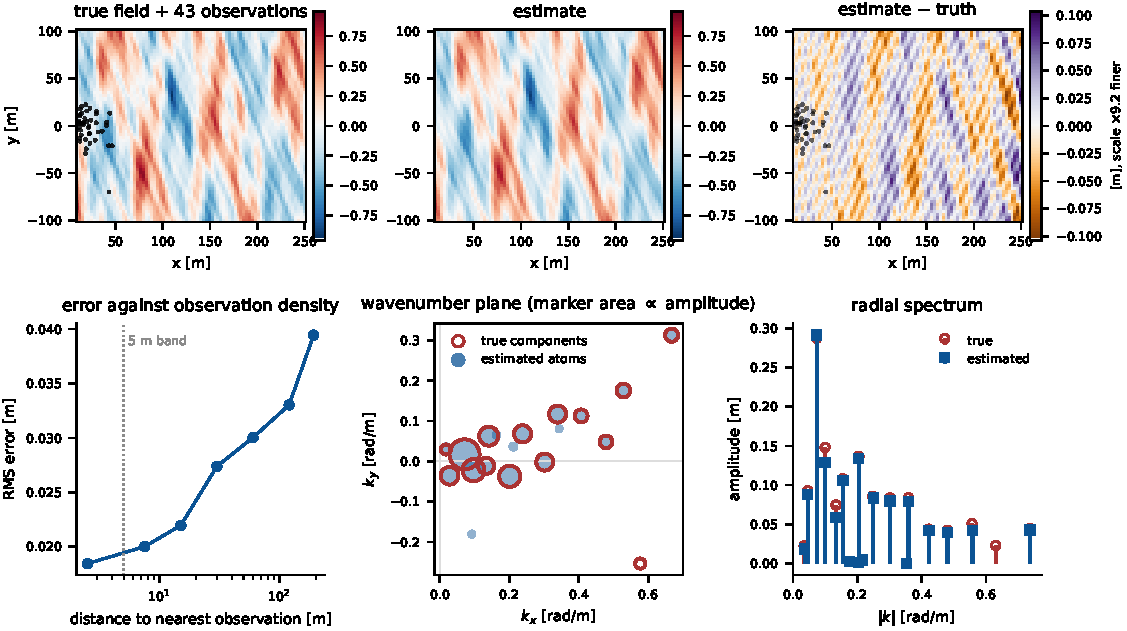
\includegraphics[width=\textwidth]{figures/fig_qualitative.pdf}
\caption{One crowded episode, one frame, illustrative only --- \emph{no comparison
is drawn here}, and every quantitative claim in this paper lives in
Table~\ref{tab:earns}. Top: the true field with that frame's observations overlaid,
the reconstruction, and their difference on a colour scale \QualScaleRatio{} times
finer (the scale factor is printed on that panel's colour bar). The
observations occupy a small patch near the sensor; the field is reconstructed across
the whole domain from the spectral parameters, which is what ``grid-free'' buys and
also where it can go wrong. Bottom left: RMS error against distance to the nearest
observation, which roughly doubles from the observed patch to the far corner ---
the error is not uniform, and a reader should not read a single domain-average
number as a local accuracy. The RMS error over this frame is
\QualFrameRmse{}~m, from \QualNObs{} observations. Bottom centre and right: the estimated atoms against the
true components. Most are recovered; the true component furthest from any estimated
atom sits at $(k_x, k_y) = (\QualMissKx{}, \QualMissKy{})$~rad/m, and the estimated
atom furthest from any true component sits at
$(\QualSpurKx{}, \QualSpurKy{})$~rad/m. The provenance of this figure --- episode,
frame, seed, configuration, and commit --- is recorded alongside it.}
\label{fig:qualitative}
\end{figure}

% ============================================================================
% ★2026-09-02 (P9) --- 4차 감사 B8. 논문 52쪽에 그림이 **하나**뿐이었고 그건 개념도다
%   (재구성 예시 0 · 오차-거리 0 · 스펙트럼 0) ⟹ 심사 가능한 증거 표면이 표 둘뿐이었다.
%   ★그림도 표와 같은 규약으로 만든다: **동결 verdict 에서만**, 손으로 적은 수 0개.
%   ★패널 (b) 는 F1 부류 공시를 **문장이 아니라 그림으로** 보인다.
% ============================================================================
\begin{figure}[!htbp]
\centering
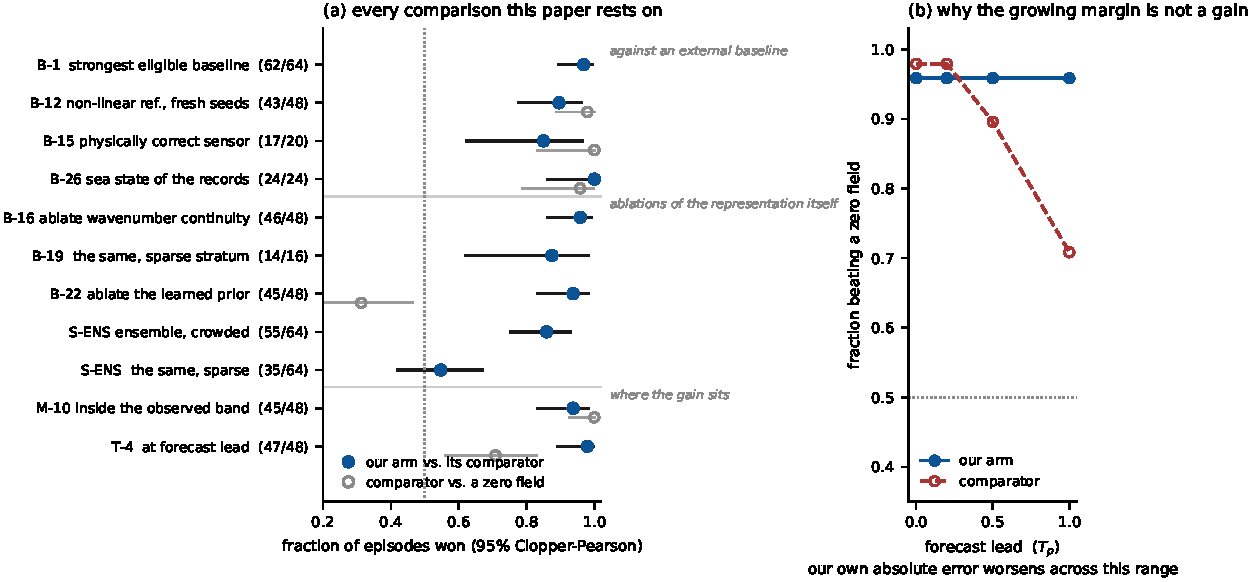
\includegraphics[width=\textwidth]{figures/fig_results.pdf}
\caption{(a) Every comparison in Table~\ref{tab:earns}, as a win fraction with an
exact $95\%$ Clopper--Pearson interval. Filled markers are our arm against the
comparator that batch used; hollow markers are that comparator against a zero
field, i.e.\ how much skill it had. Rows without a hollow marker are the ones whose
batches did not include that control. The sparse S-ENS row is the one contrast here
that does not separate. (b) Why the margin that grows with forecast lead is not a
gain: our arm's own skill against a zero field is flat across the ladder, while the
comparator's falls away, so the ratio widens because the denominator weakens.
Generated from the frozen verdict files by \texttt{scripts/gen\_fig\_results.py}.}
\label{fig:results}
\end{figure}

\subsection{A spectral-domain metric, and what it took to get one}
\label{sec:res_spectral}
% ⛔[2026-09-02] 검증 감사 MAJOR: 이것이 `\paragraph` 였고 `\label` 이 **소절 번호를
%   잡아** `\ref{sec:res_spectral}` 과 `\ref{sec:res_summary}` 가 **둘 다 5.7 로 인쇄**됐다
%   --- 그 절 안에서 그 절을 가리키니 독자가 예외를 찾을 수 없다. ⟹ 소절로 올린다.
% ============================================================================
% ★2026-09-02 (P10) --- 5차 감사 MAJOR #5 에 대한 최종 답.
%   첫 배치(`T7`)는 **자기 음성 대조가 막아** 라벨을 못 냈다. ⛔그 자료 위에서 게이트를
%   고쳐 다시 판정하면 그것이 `M-4` 에서 이 저장소가 문제 삼은 사후 완화다
%   ⟹ **다른 코퍼스**(시드 32-39, 선형 참값)에서 고친 게이트로 다시 했다(`T7b`).
%   ⚠등급은 사전등록에서 **EXPLORATORY 로 고정**했다: 첫 배치의 모든 수치를 보고 썼다.
% ============================================================================
Everything above is one metric. We add one spectral-domain measurement, and the
route to it is part of the result. Our first attempt was pre-registered and
\emph{failed its own negative control}: that design required a zero field to score
below \emph{both} arms on the two-dimensional wavenumber-spectrum $R^2$, and on a
substantial minority of episodes the analytic comparator scored below a zero field
instead --- placing energy at the wrong wavenumbers is penalised by that metric while
placing none is not. Its preregistration made that disqualifying, so it produced no
label and we do not quote its contrasts. Relaxing a gate after seeing what it caught
is the failure mode this protocol exists to prevent.

We therefore re-ran the measurement on a \emph{different} corpus --- disjoint seeds
and a linear rather than a higher-order reference --- with the control split into
three: does the metric behave, does \emph{our} arm beat a zero field, and how often
does the comparator. The first two block; the third is reported. On \SpecN{} crowded
episodes the deployed learned initialisation matches the reference wavenumber
spectrum better than the analytic one on \SpecBetter{}
($p = \SpecP{}$). \emph{We grade this exploratory and not confirmatory}, because the
first attempt's numbers were known when the second was designed.

Three things travel with it. The comparator beats a zero field on only
\SpecCmpBetter{} of the \SpecN{} episodes, so this margin is partly the comparator's
weakness and its size should not be read as an accuracy ratio. Our own arm is below a
zero field on \SpecOwnBelowZero{} episodes.
And the metric compares power spectra, which for a real field are symmetric under
$\mathbf{k}\to-\mathbf{k}$: it does not distinguish propagation direction, so it is a
spectral-magnitude agreement measure and not a directional one. The companion
amplitude-recovery contrast did not reach its threshold (\SpecHs{}/\SpecN{}) and we
draw no conclusion from it.

\paragraph{What was removed, and what that costs}
The three subsections that previously stood here --- an ablation of the dispersion
constraint and the confidence weighting, a raydrop-model sensitivity study, and a
sparsity/noise/sea-state robustness study --- together with six tables and five
figures, have been moved to the supplementary archive rather than deleted.
% ⛔[2026-09-02] 이 문장이 *"four tables and four figures"* 라 적고 있었다. **실측하면
%   `tmp/PAPER_LEGACY_2026-09-01/retracted_tables_2026-09-02.tex` 안에 표 6 · 그림 5 다**
%   (`\begin{table` 6회 · `\begin{figure` 5회 · 라벨 tab:etkf_sweep/ablation/raydrop/
%   sparsity/noise/forecast). ★처분을 세어 적었는데 그 수가 틀렸다.
Their
corpus is the one whose headline comparison is retracted, and two of them were
additionally produced before a correction to the tracker's phase advance. Where a
pre-registered replacement exists it appears in the two tables above. Where none
exists, the quantity is simply absent from this paper and we do not restate it
from the archived run: this applies to the five-metric evaluation panel, the
stratification against wave buoys, the twelve-episode comparison against tuned
grid baselines, and three sensitivity sweeps --- observation density, additive
noise, and the residual growth threshold $\tau_R$ --- whose questions remain open
rather than answered.
% ⛔[2026-09-02] 이 목록에 **밀도·잡음·$\tau_R$ 스윕 셋이 빠져 있었다** --- 바로 위
%   문장이 그 절들을 이동했다고 적으면서, 아래 목록은 그 부재를 세지 않았다.
Two items that stood in this list in the previous version have since
been re-measured and have moved out of it: a spectral-domain contrast
(Section~\ref{sec:res_spectral}, on a disjoint corpus and graded exploratory) and the
per-frame latency of the deployed learned path (Section~\ref{sec:complexity}). The
paper is thinner for this, and a reader comparing it against the
earlier version will find fewer numbers rather than more. That is the intended
direction: every number that remains is one a frozen verdict file will reproduce.

% ============================================================================
\section{Discussion}
\label{sec:discussion}

\subsection{Why a grid-free representation, and where it stops helping}
\label{sec:disc_gridfree}

% ============================================================================
% [2026-09-01 P8] 초판의 이 절(\S "Advantages of grid-free representation")을
%   tmp/PAPER_LEGACY_2026-09-01/retracted_discussion_100ep.tex 로 **옮겼다**.
%   사유: 그 절이 "복잡한 바다(15-30 성분)에서 이득이 ~5% 로 좁아진다(24/40)" 라
%   적었는데, 개정본 Results 는 **같은 층**에서 62/64, -38.6% 를 보고한다 =
%   원고가 자기모순이었다. 두 수는 다른 코퍼스에서 나왔고 옛 쪽이 철회된 코퍼스다.
%   독립 감사가 잡았다. 삭제가 아니라 이동이다.
% ============================================================================

A grid state must resolve the field everywhere it is defined, so its cost and its
conditioning are set by the resolution rather than by the complexity of the sea.
A spectral state pays instead for the number of components it carries. That is the
structural argument for the representation, and the ablations in
Section~\ref{sec:res_ablation} are what turn it from an argument into a measurement:
removing only the continuity of the wavenumber removes a margin of \BSixteenRel{},
and the loss grows when the grid is coarsened. The ablated comparator is not empty ---
it beats a zero field on \BSixteenCmpZero{}/\BSixteenN{} episodes --- and the coarser
rung does not, so that second step is a direction and not a size.
We checked separately that this ablation is not confounded with the
amplitude-and-phase refit it necessarily performs, and the magnitudes here are
\emph{not additive} with the baseline margin: they were measured on different
corpora against different comparison arms.

\paragraph{Where it stops helping, stated as measured}
The advantage is not uniform across regimes, and we no longer characterise its
regime dependence: the earlier characterisation was computed on a corpus in which
the compared arms were never scored on the same frames, and we withdraw it rather
than restate it. What we can say from the present corpora is narrower and is already
in Section~\ref{sec:res_scope}: the margin is measured on the crowded stratum;
against the deployed analytic package the sparse stratum does not separate; and on
measured records the representation does not reach the decision threshold at all.


\subsection{Effect of observation model}

% [2026-09-02 P9] 초판의 이 절은 철회된 코퍼스의 팔간 수치(15.2\% / 15.9\% / 11.7\%)를
%   실었다. 대체가 있다(B-14b, B-15) ⟹ 아카이브로 옮기고 측정된 것만 남긴다.
Two questions about the observation model have been measured on frozen batches
rather than argued. First, whether the geometric weighting of returns changes the
conclusion: it does not, and the unweighted model is in fact the more favourable of
the two (B-15, Table~\ref{tab:earns}), with the comparator retaining skill in both.
The second model was specified as a specular channel but never reaches it at this
geometry, so what was varied is the spatial weighting of returns, not the optics
(Section~\ref{sec:experiments}). Second, whether the \emph{shape} of the observation
noise explains the negative on the measured records: it does not, and the best of
four noise models still reaches only \BFourteenBBeats{}/\BFourteenBN{}
(B-14b, Table~\ref{tab:boundary}). That fraction counts records on which the arm
beats the per-record true zero-field reference; it is not a comparison between arms,
and asks only whether the arm has any skill at all. The earlier cross-arm sensitivity figures are
withdrawn with the corpus they came from and are in the supplementary archive.
\subsection{Hyperparameter sensitivity}
\label{sec:hyper}

% [2026-09-02 P9] 초판은 개발 중 스윕("100 paired runs")을 근거로 저민감을 주장했는데
%   그 100런이 철회된 코퍼스다. ⛔대체 없음 ⟹ **주장을 옮기지 않고 범위를 좁힌다.**
The four hyperparameters of the analytic path ($\text{lr}{=}0.01$,
$\lambda_1{=}\DepLambdaOne{}$, $\tau_{\text{prune}}{=}0.10$,
$\tau_{\text{grow}}{=}0.05$) were selected by a single coarse sweep during
development and then held fixed across every batch reported here --- across
Beaufort~2--5, $1$--$30$ components, several ground-truth classes, and both
strata. That one configuration was never re-tuned per experiment is a property of
the protocol and can be checked in the preregistrations; it is the only
sensitivity statement we make. The development-time perturbation sweep that the
earlier version of this section reported is not restated: it was run on the
retracted corpus and, for $\lambda_1$, at values that predate the change of the
shipped default to $\DepLambdaOne{}$. It is in the supplementary archive.
\subsection{Practical deployment considerations}

% RETRACTED 2026-08-14: 13.4 ms/frame is a banned figure (cross-process timing).
% (basis: memory/reference_citation_bans.md (08-05), (08-13 round 3))
% --- original (kept for history) ---
% WaveSplat's computational footprint (13.4~ms/frame, single CPU thread)
% makes it suitable for deployment on standard shipboard computing hardware.
WaveSplat's computational footprint on a single CPU thread
(measured in Section~\ref{sec:complexity}; an earlier figure quoted here was
withdrawn; \ref{app:changes}, R3) is intended for
deployment on standard shipboard computing hardware.  Inference does not require GPU acceleration for the tracking phase, and no offline calibration against a particular site is needed. It does require the learned proposal checkpoint at initialisation, which is where the GPU is used when one is available.
% ⛔[2026-09-02] 6차 감사 N18: 이 절이 *"배포"* 를 논하는데, \S\ref{sec:method} 의
%   라우터 공시는 **실측 입력에서 학습 경로가 아예 진입하지 않는다**고 적는다.
%   ⟹ 두 절이 서로 다른 시스템을 서술하고 있었고 논문이 그것을 화해시키지 않았다.
%   ★고치는 방향은 「배포 절을 삭제」가 아니라 **어느 시스템을 말하는지 명시**다.
\emph{Which system this paragraph is about.} The costs above are those of the
learned path, and on the synthetic corpora that is what the shipped configuration
runs. On input that carries no ground-truth field --- which is the case for real
sensor data --- the shipped router hands off to a different estimator
(Section~\ref{sec:method}), so the paragraph above describes the cost of the system
this paper measures, not of a system we have run end to end on a vessel. Making the
learned path the one that runs on real input is exactly the boundary
Section~\ref{sec:res_scope} reports we have not crossed, and we do not present the
timing as evidence that it has been.

The spectral parameters are directly interpretable: a naval architect
can inspect the estimated wavenumber vector, amplitude, and frequency
of each component, enabling sanity checking against visual observation
and meteorological forecasts.

For integration with vessel control systems, the spectral representation
offers a key advantage: the estimated wave field can be evaluated at
\emph{any} spatial point via~\eqref{eq:forward} without interpolation.
This enables downstream applications such as wave-preview feedforward
control~\citep{park2026hydrofoil}, where the wave field must be
evaluated at spatial preview points ahead of the vessel.
Grid-based methods would require interpolation between grid points,
introducing additional error and latency.

% ============================================================================
% ★2026-09-01 (P8): §6.7(strong baselines) · §6.8(spectral accuracy) ·
%   §6.9(sparse-LETKF) 를 같은 아카이브로 **옮겼다**.
%   ⛔사유: 셋 다 레거시 코퍼스 유래이고, 기준선 축은 그 뒤에 별도로 닫혔다 ---
%   ★단 그 폐쇄가 산 것은 **폐쇄이지 우월성이 아니다**(신규 4팔 중 최강 기준선이
%   된 것 0개; 최강은 여전히 스펙트럼 격자 기준선이다).
% ============================================================================

\subsection{Temporal extrapolation as validation of spectral fidelity}

% [2026-09-02 P9] 이 절의 표(tab:forecast)는 추적기 위상전개 수정 **이전** 실행이었다.
%   대체가 있다(T-4, 사전등록.동결) ⟹ 표는 아카이브로 옮기고 주장은 T-4 로 옮긴다.
Because the estimated parameters satisfy the dispersion relation by
construction, the forward model~\eqref{eq:forward} can be evaluated at any future
time without re-estimation. Whether that extrapolation is accurate is therefore a
test of the estimated $(k_x, k_y, \omega, \phi)$ rather than a forecasting
contribution, and it is reported in Section~\ref{sec:res_where} as the T-4 row of
Table~\ref{tab:earns}: at a lead of $1.0\,T_p$ the deployed path is ahead on
\TFourBetter{} of \TFourN{} episodes. That row must be read with its
negative control, because the comparator's own skill falls from
\TFourCmpAtZero{}/\TFourN{} at zero lead to \TFourCmp{}/\TFourN{} at that rung;
the rung sits at the lower end of the measured lead band, $11$ of the $12$
records. The earlier five-episode horizon table, produced before the tracker
phase-advance correction, is in the supplementary archive.
\subsection{Limitations and future work}
\label{sec:limitations}

Several limitations should be acknowledged.

\paragraph{Online model order does not contribute accuracy}
The
pruning-and-growth mechanism of the retracted corpus (archived) does select
scene-matched component counts, but under the corrected tracker its
% [2026-09-02 P10] 손타이핑 비교 철회(5차 감사 MAJOR c): §5.7 이 *"표 5/6 가 **모든**
%   비교를 모은다"* 고 적었는데 이 절에 표 밖의 철회 코퍼스 수치가 남아 있었다.
%   ⟹ 방향만 남긴다. 이 절의 어떤 계수도 재측정되지 않았다.
accuracy contribution was null on the twelve episodes it was measured on, against a
seed-to-seed noise floor far larger than the effect, and it was actively harmful on
most of the crowded ones, where the fixed energy criterion prunes to fewer
components than the scene contains.  We accordingly present it as a mechanism and a
compute-efficiency device rather than as a contribution.  A model-order
criterion that is aware of crowding---for instance, energy retention
conditioned on the beamforming main-lobe width rather than a fixed 90\%
quantile---is the natural repair and is untested.
% [2026-09-02 P9] 4차 감사 B4+B6+M8.
%   ①§5.7 이 *"buoy 층화는 대체가 없어 **다시 적지 않는다**"* 라 약속했는데 이 문단이
%     16.1/35.3/40/11.5/79.7 을 **전부 다시 적었다**(약속 위반).
%   ②⛔*"on the overlapping subset LETKF is more often better"* 는 **금지된 팔간 주장**이다
%     (금지목록 08-03·08-13 묶음; 잰 것은 합성 부분집합이고, LETKF 는 논문에 정의도 없다).
%   ③§6.1 이 *"regime dependence 를 더는 특성화하지 않는다"* 며 철회했는데
%     이 문단이 *"the regime in which this method's advantage is largest"* 로 되살렸다.
%   ⟹ 남기는 것은 **방향**뿐: 생성기가 좁은 방향확산 쪽에 치우쳐 있고 스웰이 없다.

\paragraph{Directional spread of the synthetic distribution}
Compared against a large
buoy archive, our generator occupies the lower tail of the observed
directional-spread distribution and its peak-period ceiling excludes swell, so the
synthetic universe is narrower and shorter-period than the measured one. The
per-percentile figures are not restated here: they come from the retracted corpus
and have not been re-measured. The repair belongs to the generator, not the
estimator---directional spreading functions and a $T_p$ range extending into
swell---and we deliberately did not change it mid-study so that the synthetic
results remain from one frozen dataset. We do not characterise which regime the
advantage is largest in; that characterisation was withdrawn in
Section~\ref{sec:disc_gridfree}.
% [2026-09-01] 초판은 여기서 "all results use WaveSim" 이라 적었는데, 개정본의
%   초록·Results·Conclusion 은 12 고정관측소 레코드를 보고한다 = **원고가 자기모순**이었다.
%   독립 감사가 잡았다. 아래로 정정한다.

\paragraph{The positive results are synthetic}
Every margin reported in
Section~\ref{sec:res_headline} and its ablations is measured on simulated fields
with a simulated sensor. Measured data enters this paper through the negative
in Section~\ref{sec:res_scope} and Table~\ref{tab:boundary} --- $12$ fixed-station
stereo records on which the learned prior does not reach the decision threshold ---
and through one within-arm positive in Section~\ref{sec:res_summary}, where giving
the proposal an ensemble lowers forecast error without crossing that threshold.
% ⛔[2026-09-02] 심사 B-1 의 연쇄: 이 열거가 **세 번째 진입**을 세지 않아 함께 낡았다.
It enters a third time in Figs.~\ref{fig:real} and~\ref{fig:real_qual}, which show
the same $12$ records with the deployed reference arm drawn beside the learned one;
that arm reaches ordinary significance against a zero field and, like the learned
arm, does not survive the multiplicity correction for this arc.
% ⛔[2026-09-02] 7차 심사 B9: *"**only** through the negative"* 는 거짓이다 --- §5.7 이
%   *"One positive does exist on the measured records"* 라 적는다(팔 안 대조).
Real LiDAR from a moving
platform may contain systematic biases (multi-path, spray) that neither our noise
model nor those fixed-station records represent, and no shipboard measurement of
any kind supports this paper --- the platform term was removed from the title for
that reason.

% ★★[2026-09-03] 이 절이 원고의 가장 큰 자기위협을 실었다. 심사자가 반드시 묻는다:
%   *"방금 35% 틀렸다고 잰 관측모형 아래 얻은 합성 승리를 왜 믿나?"*
%   ⛔방어 없이 두면 자해다. 반론은 있고 그것은 **내적/외적 타당도의 구분**이다.
%   ⛔`H3` 는 EXPLORATORY · 쇄파대 레짐 한정 · 추정기 런 0회. 그 셋을 같은 절에 적는다.
\paragraph{The observation model is not faithful to a real scanning LiDAR}
The synthetic corpus draws its returns from a raydrop model. We measured that model
against real returns from a Velodyne HDL-32E scanning a water surface
(\HThreeFiles{} files, \HThreeCells{} cells) under a pre-registered threshold this
project had itself written down: the mean relative error is \HThreeMRE{}, against a
threshold of \HThreeThresh{}. Two controls decide how to read that number. The
positive control shows the data carry structure the ruler can see --- measured
spread \HThreePosSpread{} against a null $95$th percentile of \HThreePosNull{} ---
so the negative is not bluntness. The negative control shows how little signal the
model has: shuffling the model across cells costs almost nothing, the shuffled
error's $5$th percentile being \HThreeShuffled{} against an actual \HThreeMRE{}, and
the rank correlation between predicted and observed return rate is
\HThreeSpearman{}. The honest reading is therefore not ``slightly wrong'' but
``almost no signal in this regime''. The measurement is exploratory, it ran no
estimator, and its regime is a surf zone rather than the deep water the synthetic
corpus represents --- a transfer that runs in the unfavourable direction and that we
do not resolve.

We also asked whether the failure lies in the radiometric quantity or in the
detection law applied to it. Holding that quantity fixed and replacing the
multiplicative-gain law by the threshold-with-speckle law the same simulator already
ships --- one free parameter each, fitted by the same median-matching rule --- lowers
the error by \HThreeCRel{}, from \HThreeCMreA{} to \HThreeCMreC{}, which is still far
above the threshold and only \HThreeCShufC{} away from that law's own shuffled null.
A third shipped variant is excluded before the fact because its specular gate never
fires at this geometry. None of the three is faithful, so the remedy is not to select
a different one of them; the remaining suspect is the radiometric term itself, whose
incidence-angle dependence the simulator's own source comments already flag as
inverted relative to what the surrounding text claims. This comparison is exploratory,
it was not blind --- a first attempt was blocked by two mis-specified gates of ours and
the statistics were seen while diagnosing that block --- and it inherits the surf-zone
regime.

What this does and does not undermine matters. Every ablation in
Section~\ref{sec:res_ablation} compares two arms \emph{under the same observation
model}, so the internal comparison --- which component carries the accuracy --- is
untouched by an error common to both arms. What the measurement bounds is external
validity: the claim that a margin measured under this observation model would appear,
with this sign and this size, on returns from a real scanning sensor. We make no
such claim, and this is the second independent reason (after the synthetic reference
field) why the margins in this paper are not transferable numbers.

% ★[2026-09-03] `R8-HELDOUT`. ⛔명목이다(확증 11 에 한 표 모자람) · ⛔SEC-LARGE 3/5 병기 의무 ·
%   ⛔기제 지목 금지 · 완전 blind 아님(스모크 1 레코드 2 셀).
\paragraph{On measured records the scoring sits largely inside the observation support}
On the fixed-station records the query points are close to the observations: the
gap to the nearest observation is a few hundredths of a peak wavelength. To ask what
that is worth, we confined the observations to one half of each box and scored the
same single estimator run on two disjoint query subsets --- inside the observed half
and outside it. Aperture, observation count, seed and initialisation are then
identical by construction and only the scoring region differs. Skill is present
inside on \REightSkillIn{}/\REightN{} records and outside on only
\REightSkillOut{}/\REightN{}; the median ratio to a per-record zero field moves from
\REightRatioIn{} to \REightRatioOut{}, that is, to no skill. The paired direction
holds on \REightBetter{}/\REightN{} records ($p = \REightP{}$), which clears the
nominal threshold but not the confirmatory one. \emph{It also fails to reproduce in
the stratum with the most query points}: on the \REightBigN{} records whose box
exceeds $40$\,m it holds on \REightBigW{}, so we cannot exclude that larger apertures
hold up outside their support. We report the split rather than the primary alone, we
name no mechanism, and one record of twelve was seen in a smoke test before the batch
was frozen.

% ★[2026-09-03] `R7-FLOOR`(신규 런 0회, EXPLORATORY, blind 아님, 사이트 1개).
%   ⛔보정된 nRMSE 를 만들지 않았다 · ⛔PROP 을 구제하지 않는다.
\paragraph{Part of the measured error is charged for content the model class cannot represent}
The reference surface against which the measured records are scored is itself a
reconstruction, and an independent instrument bounds its high-frequency excess. Across
the \RSevenN{} records that carry a co-located wave-gauge array, that bound --- expressed
in units of the record's own standard deviation --- predicts how much skill the deployed
arm retains, with a rank correlation of \RSevenRho{} ($p = \RSevenP{}$, exhaustive
permutation, against a minimum detectable $\rho$ of \RSevenMDE{} at this sample size).
The control matters more than the correlation: the same bound is uncorrelated with the
no-skill zero reference ($\rho = \RSevenCtrlRho{}$, $p = \RSevenCtrlP{}$), so this is not
the restatement that noisier records have larger everything. Since the excess lies above
$1$\,Hz and the peak periods here are $2.5$--$5.7$\,s, it is variance a sum of at most
fifteen plane waves cannot represent, and the scoring charges the estimator for it. This
is exploratory, it was not blind, it rests on one site, its bound is an upper bound, and
it does not rescue the learned prior --- the same correlation on that arm is null. We
therefore report it as a caveat on how the measured negatives should be read, and we do
not construct a corrected error from it.

% ★[2026-09-03] 조선해양공학 적대적 심사가 찾았다: **예보 지평의 붕괴가 저장소에 측정돼
%   있는데 두 원고에 0회**였다. 조선 독자에게는 가장 중요한 수다.
%   ⛔사전등록 판정이 아니라 **동결 행의 런 0회 재집계**(RV4_adversary.md)임을 밝힌다.
%   ⛔대상은 배포 실측 팔(bank, 고정 적합)이지 학습 사전이 아니다. `REFIT2` 는 붕괴하지 않는다.
\paragraph{The forecast horizon on measured data ends inside two wave periods}
Beyond a lead of about five seconds the frozen-fit real-data arm stops predicting rather
than degrading gracefully. Measured as the ratio of predicted to true field variance, and
calibrated against a positive control that must return one by construction (it returns
$0.82$--$1.92$, median $\approx 1$), that arm's predicted field holds $0$--$17\%$ of the
true variance at leads of five seconds and beyond: it is effectively outputting zero. The
measured records have a median peak period of about $3.5$~s, so the skill ends at roughly
$1.2$ wave periods --- inside the one-to-two-period horizon that shipboard operations
would need. Three qualifications travel with this. It is a re-aggregation of frozen rows
rather than a pre-registered contrast, and the ratio is an upper bound. It is a property
of the \emph{frozen-fit protocol}: the arm that refits every two seconds does not
collapse. And the arm in question is the deployed bank estimator, not the learned prior
this paper is named for --- which, as Table~\ref{tab:boundary} records, does not reach
the threshold at any lead including zero.

% ★[2026-09-02] `R4b` --- *"왜 12 레코드뿐인가"* 에 **측정으로** 답한다.
%   ⛔정확도 주장 아님(추정기 런 0회) · ⛔*"자료가 나쁘다"* 아님 · ⛔기제 지목 금지 ·
%   ⛔사이트 일반화 금지. 동결 = `verdict_r4b.json`(게이트 11/11).
\paragraph{The measured corpus is small because the candidate we checked is out of
regime} The twelve records come from four fixed stations, and the obvious way to
enlarge that set --- another public stereo reconstruction --- did not survive an entry
check that this paper's own hard constraint imposes. For each record we measured the
fraction of wavenumber-ring energy lying within three frequency bins of the linear
dispersion surface, and compared it against a null that applies the identical counting
geometry to a \emph{displaced} surface, so that each record is judged against itself.
All \RFourBCtrlPass{}/\RFourBCtrlN{} of our records exceed their own null. Of the
records from a shipborne Antarctic stereo campaign, \RFourBTreatPass{}/\RFourBTreatN{}
do: their observed fractions reach at most \RFourBTreatMax{}, about six times below the
weakest of ours (\RFourBCtrlMin{}). \textbf{This is a non-exceedance, not an absence.}
On the same records the observed fraction sits above the \emph{median} of its own null
on six of six, so what we can say is that the concentration does not clear the null's
$95$th percentile --- not that no dispersion structure is present. One confound is
disclosed rather than resolved: the Antarctic records all have a $0.5$~s sample interval
against $0.067$--$0.1$~s for ours, and the null's counting geometry self-overlaps more
often at the coarser interval, which raises that group's threshold. The artefact pushes
in the direction of the reported outcome, so we measured it rather than argue about it:
recomputing every threshold with each frequency bin counted once --- the observed values
are bit-identical under that change --- moves the Antarctic thresholds by
\RFourCDropMed{} at the median, and the counts do not move at all
(\RFourCCtrlPass{}/\RFourBCtrlN{} and \RFourCTreatPass{}/\RFourBTreatN{}). For a record
to change side its threshold would have to fall by more than three quarters. The
sampling-interval confound is real in direction and too small in size to carry the
result; the other channels through which it could act are not measured here. We do not claim those data
are poor, and we do not name a mechanism --- uncompensated platform motion and swell
longer than the reconstructed patch are not separable from the surface field alone. We
report only that a hard dispersion constraint is not a description of that sea, so
adding it would not enlarge the corpus this estimator addresses.
% CORRECTED 2026-08-14: 39 -> 196 unit tests (measured 2026-08-13; 85 wavesim +
% 111 wavesplat, three agents ran it independently), plus 8 shipping-default
% regression tests added on 2026-08-13.
% SCOPE: the "Gerstner kinematics" test exercises the single_gerstner() FUNCTION;
% the generation pipeline discards that function's displacement output, so the test
% does NOT certify that the generated data is nonlinear.
% (basis: memory/project_audit_recheck_2026-08-13.md sections 1, 6, 6.5)
% --- original (kept for history) ---
% We note that the simulator itself is validated by 39 unit tests
The simulator and estimator carry an automated test suite
(\DeployNumTestsPaper{} tests, counted by a collection run rather than typed)
covering dispersion, Gerstner kinematics, Fresnel optics and raydrop statistics;
\emph{it does not certify that the generated data is non-linear}, because the
Gerstner test exercises a kinematics function the generation pipeline does not use
for horizontal displacement.
% ⛔[2026-09-02] 6차 감사 N4: 여기 *"(measured 2026-08-13; a further 8 ... added
%   subsequently)"* 가 겹쳐 붙어 있었다. 수를 **손으로 적던 시절**(204)의 잔재다.
% ★[2026-09-02] 8차 검토: 세 문장을 하나로 접었다(내용 동일).
% ============================================================================
% ★2026-09-02 (P10) 5차 감사 REJECT 급. 이 자리에 있던 문장은
%   *"the 100-episode evaluation across 5 seeds, 10 configurations, and 2 observation
%   models provides a level of statistical rigour…"* 였다.
%   ⛔**그 설계가 바로 철회된 코퍼스다** --- §4.1 이 *"belongs to the retracted corpus and
%   is not used here"* 라 적고, Data availability 가 *"The headline results were not"*
%   그 코퍼스에서 나왔다고 적는다. ⟹ ★**논문의 엄밀성 주장이 자기가 철회한 것에
%   기대고 있었다.** 삭제하고, 실제로 가진 근거로 대체한다.
% ============================================================================
What the protocol does provide instead is narrower and checkable: each comparison
in Section~\ref{sec:results} is paired per episode, its direction and decision
threshold fixed before results existed, its analysis code checksum-frozen (with the
one exception noted there), and its number read from the resulting verdict file
rather than transcribed. Like the LiDAR-based studies that preceded
us~\citep{desmars2020, desmars2023jfm}, we establish the algorithm in simulation
first; unlike a tank trial, simulation cannot tell us whether the result transfers,
which is what Table~\ref{tab:boundary} is for.
% RETRACTED 2026-08-14: this fairness argument is FALSE and was the single most
% load-bearing false statement in the manuscript.
% wavesim/gt_generator.py:38 reads
%   `_, _, Z, NX, NY, NZ = single_gerstner(...)`
% -- it discards the two horizontal displacement components and returns elevation only
% (verified by direct reading 2026-08-14). wavesim/pipeline.py:157,165 build both the
% ground-truth field and the raycast mesh from that function, so the Gerstner steepness
% parameter Q enters neither. Reconstructing the stored gt_wave_field as
% Sum_i A_i cos(kx_i x + ky_i y - w_i t + phi_i) gives max|delta| = 0.000e+00 on four
% episodes spanning sparse, crowded and public corpora.
% Consequences: (a) the mismatch is not O(eps^2), it is exactly zero, so "<0.5%" is void;
% (b) a mismatch of zero is NOT "equal for all methods" -- the grid-based methods do not
% use that representation, so a zero mismatch favours the plane-wave estimator.
% Nonlinear validation was done in a separate HOS (M=3) batch, not on this corpus.
% (basis: memory/project_audit_recheck_2026-08-13.md section 6.5 ·
%  memory/reference_citation_bans.md (08-13 round 3) ·
%  memory/project_hosgate_result_2026-08-13.md · direct code reading 2026-08-14)
% --- original (kept for history) ---
% The ground-truth wave field uses Gerstner (nonlinear) kinematics while
% all estimation methods---WaveSplat, ETKF, LETKF, GPR---use a linear
% forward model; therefore the $O(\epsilon^2)$ model mismatch affects
% all methods equally and does not bias the comparison.
% 

% ⛔[2026-09-02] 검증 감사가 잡은 인쇄 손상 둘, **둘 다 오늘 내 수리가 만들었다**:
%   ①`5ccf8fbf` 가 주석 조각을 `\paragraph` 로 풀었고 `91859029` 가 그 자리를 메우던
%     `[RETRACTED]` 블록을 치워 **술어 없는 문장**이 인쇄됐다
%     (*"The O(eps^2) mismatch is (App. …, R2.) The correct facts are: …"*).
%   ②그 결과 `\paragraph{Linear forward model}` 이 **연달아 두 번** 인쇄됐다.
%   ★같은 부류가 오늘 초록에서도 났다(금지 자구 교체가 `is` 를 남겼다).
\paragraph{Linear forward model}
The synthetic ground truth is a \emph{displacement-free linear superposition on a
fixed grid}, so it lies in the same function space as the estimator's model equation
and the measured mismatch is \emph{zero} --- and a zero mismatch is not neutral
between methods, because the grid-based baselines do not use that representation.
(An earlier claim that the mismatch was small but non-zero, and equal across methods,
is withdrawn: \ref{app:changes}, R2.) The linear approximation does
degrade for steep waves, and a second-order Stokes extension would preserve the
spectral parameterisation. \emph{Non-linear validation was performed in a separate
higher-order-spectral ($M{=}3$) batch, not on this corpus.}

\paragraph{Tracking phase dependence on initialization}
The \texttt{w\_phi} tracking mode freezes wavenumbers and updates only amplitudes
and phases, so whatever the initializer misses is unrecoverable thereafter: tracking
quality is capped by initialization quality, regardless of why a component was
missed. Measured on the re-scored corpora, tracking ends slightly above its own
initialization on most arm--episode pairs, by a small and bounded margin. So the
honest characterisation of Phase~2 is not that it degrades the estimate but that it
holds the initialization roughly in place at a fraction of the per-frame cost.
\emph{Tracking is a compute mechanism, not an accuracy mechanism.} Two earlier
descriptions of this limitation --- a beamforming detection threshold at
$|k|\gtrsim 0.4$~rad/m, and a $2$--$3\times$ inflation of tracking error --- were
withdrawn; both were properties of the superseded rendering mesh rather than of the
algorithm (\ref{app:changes}, R6).
% ★[2026-09-02] 8차 검토: 이 문단이 **30 인쇄줄**로 §6.6 에서 가장 길었고, 그중 약 22줄이
%   **철회된 주장의 서사**(메시 독립 시험 · 0.4 rad/m · 2-3배 · 0.009→0.08)였다.
%   ⟹ 살아 있는 **구조적 한계**만 남기고 철회 서사는 부록 `R6` 으로 옮긴다(삭제 아님).
% ★2026-09-02 (P10) 5차 감사 MAJOR: §4.3 이 *"네 부차 지표는 재측정되지 않았다"* 라
%   적었는데 이 문단이 VR 값 셋(0.916/0.910/0.925)을 **현재형으로** 인용했다.
%   ⟹ 값을 빼고 **방향**만 남긴다(그 방향은 철회 대상이 아니다).

\paragraph{Residual amplitude under-estimation}
The estimator recovers less variance
than the true field, and on the retracted corpus that deficit did not differ between
the sparse and crowded halves even though nRMSE did. The levels are not restated
here: variance ratio was part of the secondary panel that was not re-measured for
the batches reported in Section~\ref{sec:results}. An earlier attribution of the
deficit to Adam momentum is withdrawn (\ref{app:changes}, R7); what remains is
\emph{unattributed} --- we can observe it but not currently explain it, and we prefer
to say so rather than carry forward a mechanism whose named cause no longer exists.
% ⛔[2026-09-02] 6차 감사 N17: 이 문단은 세 문장 위에서 *"The levels are not restated
%   here"* 라 적고 세 문장 뒤에 **0.66 / 0.83 / 0.916 / 8\%** 를 다시 적었다.
%   5차 감사가 같은 결함을 이웃 문단에서 잡았고 **처방이 이 문단에 적용되지 않았다**
%   (N-1 부류, 오늘 여덟 번째). ⟹ 값 넷을 빼고 방향만 남긴다.
% ⛔[2026-09-02] **주석이 본문을 삼켰다** — 아래 한 줄이 그 복구분이다.
Post-hoc
least-squares amplitude calibration is effective when dense observations
are available but does not improve with sparse LiDAR ($\sim$50~pts/frame)
due to insufficient spatial coverage; isolating the residual mechanism
(momentum-free optimizers for amplitude, periodic optimizer state resets,
or a per-frame amplitude least-squares solve) is future work.

\paragraph{Initialization resolution and the peak-separation radius}
The greedy
beamforming peak search enforces a fixed minimum separation
$\Delta k_{\min}=0.15$~rad/m between accepted peaks, so component pairs closer
than this in wavenumber space are structurally unresolvable by our initializer
% [2026-09-02 P9] 4차 감사 M15: 코퍼스는 어디서나 **100 에피소드**인데 이 줄만 195 다.
%   ⛔출처를 확인할 수 없다(철회 코퍼스 계열의 확장 집합으로 보인다) ⟹ 비율을 빼고
%   **검증 가능한 형태**로만 남긴다: "모든 15/20/30 성분 에피소드" 는 구성에서 따라온다.
% ✅[2026-09-02] 전칭 검증: `config/wave_components` 의 (kx, ky) 로 최근접 쌍 거리를
%   계산하면 15/20/30 성분 에피소드 **88/88** 에서 0.15 rad/m 미만 쌍이 존재한다
%   (`data_finemesh_2026-07-23` + `HOSGATE/data_hos`, 런 0회). 반례 0.
regardless of signal-to-noise ratio.  This is not a corner case: a majority of the
simulated episodes---and every 15-, 20- and 30-component episode---contain at
least one true pair separated by less than $0.15$~rad/m. (The exact count came from
the retracted corpus and is not restated.)  A pre-registered sweep of
$\Delta k_{\min}$ shows the constant to be a regime-dependent trade rather than a
universal floor --- relaxing it helps the crowded case and hurts the sparse one, in
every seed of each --- so two things follow. The crowded-regime error is \emph{not}
explained away by this constant: the bulk of it survives when the constant is
removed. And statements of the form ``these components are not recovered'' are
properties of the estimator \emph{as configured}, not method-independent
impossibility. The sweep's magnitudes are not restated (retracted corpus, not
re-measured) and the sweep design is in \ref{app:changes}, R8; the principled repair
is an adaptive radius scaled to the beamforming main-lobe width, which we have not
tested.
% ★[2026-09-02] 8차 검토: 25 인쇄줄 중 스윕 **설계 서술**과 수리 제안이 절반이었다.
%   살아 있는 두 귀결만 남기고 설계는 부록 `R8` 로 옮긴다(⛔삭제 아님).
%   ⚠`for N>=30` 문장은 이 한계의 **다른 축**(격자 분해능)이라 부록으로 함께 보낸다.

\paragraph{Current estimation}
We do not estimate ocean currents, whose
Doppler shift makes the apparent dispersion
$\omega=\sqrt{g|k|\tanh(|k|d)}+\mathbf{k}\cdot\mathbf{U}$; a
0.5~m/s current introduces ${\sim}5\%$ frequency bias at BF4.
Joint current--wave estimation is a natural extension.

\paragraph{Cold start and re-initialization}
Phase~1 requires
$T_{\text{init}} = 2T_p$ of observations (e.g., $\sim$16~s at BF4)
before tracking begins; during this interval no wave estimate is
available.  If the sea state changes abruptly (e.g., vessel course
change exposing a new swell system), re-initialization is needed,
incurring the same latency.  A background re-initialization scheme
running in parallel with tracking could mitigate this in practice.

\paragraph{Surface normal approximation for real data}
In simulation
we use the exact surface normal of the reference field for confidence weighting
(that field is a displacement-free linear superposition, not a Gerstner surface;
see Sections~\ref{sec:obsmodel} and~\ref{sec:experiments})
$c_j$, but real-data application must substitute the flat-surface
approximation $\mathbf{n}\approx\hat{\mathbf{z}}$.  The resulting
bias scales with wave slope (up to ${\sim}9\%$ in $\cos\theta_j$
at grazing incidence at BF4); wave-tank validation is planned to
characterise the end-to-end nRMSE impact.

\paragraph{Observation weight nomenclature}
The weighting $c_j = \cos\theta_j/(r_j/d_{\text{ref}})$ is a geometry-aware
simplification, not the exact Fresnel reflectance~\citep{born1999}, which would
require surface-roughness and polarisation assumptions we cannot justify from
observation alone. The name follows the functional form.
% ★[2026-09-02] 8차 검토: *"previously 'Fresnel-aware' in an earlier draft"* 는
%   **한계가 아니라 편집 이력**이다 ⟹ 부록의 철회표가 담당한다(R1 의 같은 기제).
% [2026-09-02 P9] 4차 감사 B5. ⛔이 문단은 **철회된 코퍼스를 긍정 근거로** 썼다
%   (*"show our conclusions hold under the best baseline configurations"*).
%   그것은 §5.7 이 하지 않겠다고 약속한 바로 그 행위이고, 측정과도 어긋난다
%   (수리된 기준선 대비 PRIMARY 는 `UNDECIDED`).

\paragraph{Baseline fairness}
We cannot claim to have beaten a fully tuned ensemble
filter. The sweep and cross-baseline comparisons that once supported such a claim
were run on the retracted corpus, and the one pre-registered attempt to re-establish
it against a repaired baseline returned an undecided primary. What survives is the
narrower statement of Section~\ref{sec:res_headline}: the comparator there is the
strongest eligible baseline we possess, not a baseline strengthened for the
occasion. Further tuning of ensemble filters, or hybrid ensemble--spectral
approaches, remain unexplored.

\paragraph{Uncertainty quantification}
WaveSplat returns point estimates;
Hessian-based confidence intervals or multi-start ensembles could
provide uncertainty.

\paragraph{Directional spreading}
Each component is monochromatic;
representing continuous directional distributions (e.g., $\cos^{2s}$)
would require directional or von~Mises basis functions.

\paragraph{Ship motion}
The current simulation assumes a stationary
sensor platform.  In practice, heave, pitch, and roll of the vessel
change the LiDAR beam pattern frame-to-frame; an IMU/INS-based
coordinate transform is a necessary preprocessing step for
sea-going deployment, and the residual motion-compensation error
constitutes an additional noise source not modelled here.

\paragraph{Near-surface false returns}
At 1550~nm the absorption length
of sea water is approximately 1~mm~\citep{hale1973}, so essentially
no light penetrates below the surface; sub-surface volume scattering
is negligible.  However, sea spray, whitecaps, and rain droplets
above the nominal water surface can generate false LiDAR returns
that are indistinguishable from surface elevation measurements.
These super-surface returns introduce a positive elevation bias
not captured by the additive noise model, and their prevalence
increases with sea state; empirical calibration on real data is
needed to assess their impact.

\paragraph{Relationship to physics-informed learning}
The division of labour here is worth stating plainly, because the two halves are
often conflated. The \emph{basis} is hand-designed: plane waves that satisfy
dispersion by construction rather than as a soft penalty, carrying $4N$ parameters
rather than a network's --- which matters with $\sim$50 observations per frame. What
is \emph{learned} is not the basis but the \emph{selection}: which atoms to place,
as a set, from one observation window. WaveSplat is therefore physics-constrained
optimisation, structurally analogous to PINNs with a neural basis, while WavePrior
supplies the initialisation that neural bases lack. The ablation of
Section~\ref{sec:res_ablation} separates the two: with the basis intact and the
learned selection replaced by an analytic one \emph{and nothing else changed}, the
arm clears a zero predictor on only \BTwentyTwoAnaZero{}/\BTwentyTwoN{} episodes.
% ⚠[2026-09-02] 이 자리의 15/48 은 **옳다** --- 단일요인 교체(`L1a`, 우변 `ANA`)를
%   서술하기 때문이다. `L2`(우변 `ANA-SHIP`, 32/48)와 혼동하지 않도록 자구를 좁혔다.
% ★[2026-09-02] 8차 검토: 이 문단은 **한계가 아니라 관련 연구**다. 다음 개정에서
%   \S2 로 옮기는 것이 옳다 --- 지금은 압축만 한다(절 이동은 참조 그물을 건드린다).

% ============================================================================
\section{Conclusion}
\label{sec:conclusion}

% ============================================================================
% ★2026-09-01 (P8) 재작성. 초판 결론은 철회된 헤드라인(0.115 / 0.332 / 65.5%)을
%   그대로 담고 있었다. ⛔모든 수는 paper_constants.tex 매크로다.
% ============================================================================

We estimate phase-resolved ocean wave fields from sparse 3D point clouds as a small
set of continuous-wavenumber spectral atoms under a dispersion constraint, with the
initial configuration proposed by a learned set-valued prior.
% ★2026-09-02 (P10) 5차 감사 권고 2d --- 초록과 같은 이유로 결론도 `B-12` 를 앞세운다:
%   *"the paper states a mandatory control, then leads with the row that lacks it."*
On crowded multi-component \emph{synthetic} seas with a higher-order reference field
(\HosCrowdedDegraded{} of \HosCrowdedN{} episodes realise it at second rather than
third order) and previously unused
seeds, this lowers median normalised RMSE by \BTwelveRel{} against the strongest
eligible grid baseline we possess (\BTwelveBetter{}/\BTwelveN{} episodes), in a
comparison where that baseline itself retains skill against a zero predictor
(\BTwelveCmpBetter{}/\BTwelveCmpN{}).

What we regard as the substantive contribution is not the margin but the
\emph{attribution}. Holding the deployed pipeline fixed and removing one property at
a time, the learned prior accounts for \BTwentyTwoRel{}
(\BTwentyTwoBetter{}/\BTwentyTwoN{}) --- measured against an analytic package that itself
clears a zero predictor, though thinly (\BTwentyTwoAnaShipZero{}/\BTwentyTwoN{}, $p = \BTwentyTwoAnaShipZeroP{}$)
--- and the continuity of the wavenumber accounts for \BSixteenRel{}
(\BSixteenBetter{}/\BSixteenN{}, dose-responsive, and reproducing in the sparse
stratum at \BNineteenBetter{}/\BNineteenN{}). The gain also survives
re-scoring inside the observation-density band our measured records occupy
(\MTenBetter{}/\MTenN{}) and at a forecast rung that $11$ of those $12$ records cover (\TFourBetter{}/\TFourN{}) --- though in the latter case the comparator
degrades across the same interval, so the growing ratio must not be read as a
growing advantage.
% [2026-09-01] 공시 검사기 요구: rung 범위 · blind 아님 · B-16 교락 · 비가법.
Neither re-scoring was blind --- the expected direction was known before the runs,
so they are not blind replications --- and that rung sits at the lower end of the
measured lead band rather than spanning it. The two ablation magnitudes are \emph{not
additive} with each other or with the baseline margin --- different comparison arms,
and in the baseline's case a different corpus as well --- and we verified separately that the grid-snapping
ablation is not confounded with the refit it necessarily performs.

\paragraph{What we did not obtain}
On $12$ fixed-station stereo records the learned prior does not reach the
pre-registered threshold against a per-record zero-field reference under any arm
configuration we tested, including one in which it is given the same median-of-$k$
field ensemble that the deployed real-data path uses --- a path in which, in the
shipped configuration, the prior is not invoked at all
(Section~\ref{sec:method}). That treatment does lower
error by a confirmed margin and does move the endpoint, but not across the
threshold. We state this as a measured boundary rather than as an omission: the
representation that earns its gain on crowded synthetic seas has not been shown to
earn it on the measured data we hold, and locating that boundary --- rather than
widening the margin --- is where we believe the remaining work lies.

We also note two limits of the evidence itself. Every comparison against a grid
baseline in this paper is on the crowded stratum. In the sparse stratum the evidence
is split rather than absent: the wavenumber-continuity ablation reproduces there
(\BNineteenBetter{}/\BNineteenN{} episodes), while against the deployed analytic
package the stratum does not separate. Those are two different comparators and
neither answers for the other.
% ⛔[2026-09-02] 6차 감사 N11: 초록.\S5.4.결론이 **세 개의 서로 다른 참인 문장**을
%   *"crowded-stratum only"* 하나로 뭉쳤고, 그 하나를 **표 5 의 B-19 행이 반증**한다
%   (희소 14/16). ★한 문장으로 접을 수 없는 것을 접으면 자기 표와 충돌한다.
And the learned checkpoint was trained on the same distribution family
as the synthetic evaluation, so ``out of sample'' on that corpus means on the seed
axis only.


\section*{CRediT authorship contribution statement}

The sole author is responsible for all aspects of this work.

\section*{Declaration of competing interest}

The author declares no known competing financial interests or
personal relationships that could have appeared to influence
the work reported in this paper.

% ★2026-09-02 (P10) --- 5차 감사 최우선 권고: 철회 이력을 본문에서 부록으로.
\appendix
% ⛔손으로 고칠 때는 본문의 포인터(App. R1..R4)도 함께 고쳐라.
%   ★이 부록이 존재하는 이유(2026-09-02, 5차 감사 축자):
%   *"after the fourth [RETRACTED] tag in running prose, the tags stop reading as
%    candour and start reading as an unfinished edit log left in the manuscript.
%    Move the retraction history to a numbered appendix … That single change would
%    convert the paper's greatest liability into its greatest asset."*
\section{Changes from earlier versions}
\label{app:changes}

Earlier versions of this manuscript made four claims that later measurement
withdrew. We list them here rather than in the running text, so that the body states
only what is currently supported; each is referenced from the section where the
claim used to appear.

\begin{table}[!htbp]
\centering
\footnotesize
\caption{Withdrawals and corrections, with what replaced them.}
\label{tab:changes}
\begin{tabular}{lp{0.30\columnwidth}p{0.44\columnwidth}}
\toprule
& Withdrawn & Why, and what stands now \\
\midrule
\textbf{R1} & Geometry-aware confidence weighting as a \emph{contribution}
(2026-08-14) &
A fresh out-of-sample corpus found disabling the weighting better in both strata.
The mechanism is still deployed and still described, because a later ablation
found that \emph{removing} the ground-truth-derived weighting also hurts; what
does not stand is calling it a contribution of this work. \\
\addlinespace
\textbf{R2} & ``The ground truth is Gerstner (non-linear), so the
$O(\epsilon^2)$ mismatch affects all methods equally'' (2026-08-14) &
False on both halves. The generator discards the horizontal displacement, so the
reference field is a displacement-free linear superposition and the measured
mismatch against the model equation is exactly zero. The non-linear case is now
measured separately with a higher-order reference
(Section~\ref{sec:res_hos}). \\
\addlinespace
\textbf{R3} & All absolute per-frame latencies (2026-08-14) &
They came from separate processes without thread pinning, so they measured the
harness as much as the estimator. \emph{Superseded}: the deployed path has since
been timed in one process on a single thread and is reported in
Section~\ref{sec:complexity}. No baseline arm was timed, so no comparative timing
claim replaces the withdrawn ones. \\
\addlinespace
\textbf{R4} & ``The dispersion constraint contributes accuracy''
(2026-08-14) &
The ablation that supported it removed the frequency initialisation together with
the constraint, so it did not isolate either. What stands is the parameter-count
reduction, which is structural. A controlled intervention has not been run. \\
\bottomrule
\end{tabular}
\end{table}

A fifth class of change is not listed above because it is not a withdrawal of a
claim but of a \emph{corpus}: an earlier evaluation corpus was found to score the
compared arms on different frames, and every cross-arm number computed on it has
been removed from this paper. Section~\ref{sec:res_summary} states which quantities
had a pre-registered replacement and which are simply absent as a result.


\section*{Data availability}

% [2026-09-02 P10] 5차 감사: ①**체크포인트가 배포 목록에 없었다**(제목이 파는 것이다)
%   ②*"the frozen corpora **named in** Section 5.1"* --- §5.1 은 아무것도 명명하지 않는다.
Code, simulation data, experiment scripts, \emph{and the trained prior checkpoint}
will be deposited on a public repository upon acceptance. Every result in
Section~\ref{sec:results} carries a batch identifier (B-1, B-12, \dots); each names
a directory in that repository holding its preregistration, its checksum-frozen
analysis code, its raw result rows, and the verdict file from which this paper's
numbers are read. Two figures are exceptions and are marked where they appear: the
sparse re-aggregation of Section~\ref{sec:res_scope}, which is recomputed from
W-15's frozen rows rather than read from its verdict, and the illustrative frame of
Fig.~\ref{fig:qualitative}, which carries its own provenance record instead.
% [2026-09-02 P9] 4차 감사 M17: 본문이 "supplementary archive" 를 **다섯 번** 가리키는데
%   그것이 무엇인지 어디에도 없었다. 실체는 저장소 안의 이동 대상 파일이다.
The ``supplementary archive'' referred to in Sections~\ref{sec:res_summary}
and~\ref{sec:discussion} is a single directory in that repository holding the
subsections, tables, and figures withdrawn from this manuscript, kept verbatim with
the reason for each withdrawal, so that a reader can see what was removed rather
than only that something was.
The complete 100-episode dataset can be regenerated from the released
simulator with the provided configuration files and fixed random
seeds, ensuring end-to-end reproducibility of the tables and figures that were
computed on it. The headline results of this paper were \emph{not} computed on that
dataset: they come from the frozen corpora of the batches identified in
Table~\ref{tab:earns}. The two checkpoints the deployed learned path loads are in the
same repository and are identified here by digest --- the conditional denoiser
(\texttt{\CkptShaFull{}}) and the normalisation prior
\texttt{setdiff\_prior.pt} (\texttt{\PriorCkptShaFull{}}) --- so a reader can verify
that the released weights are the ones these numbers came from.

The buoy directional-spread statistics used for the external-validity
stratification of the retracted corpus (archived) are third-party
observations from the Coastal Data Information Program~\citep{cdip},
retrieved over OPeNDAP on 2026-08-03.  We release the station list, the
pre-fixed sampling rule, the retrieval and estimator scripts, and the
derived per-record spread values, so that the stratification is
reproducible without redistributing CDIP data.

% [2026-09-01] 초판 문장 "We were unable to validate on measured data" 는 이제 거짓이다
%   --- 개정본은 12 고정관측소 스테레오 레코드 위의 **음성**을 보고한다. 정확히 무엇을
%   못 찾았는지로 좁힌다(못 찾은 것은 **LiDAR** 자료이지 실측 자료 일반이 아니다).
We could not locate a public, phase-resolved, two-dimensional \emph{lidar}
sea-surface dataset, and we state the scope of that search rather than assert
non-existence. The measured evaluation in this paper therefore uses stereo
reconstructions from fixed stations rather than lidar, which is itself a scope
limit: the sensor that motivates the method is not the sensor the negative result
was obtained with.  We
enumerated the collections of the USACE Field Research Facility THREDDS
server to collection level---its \texttt{frf/} and \texttt{projects/}
trees and the nine collections at the server root---and found one
candidate, a 30-file, three-day scanning-lidar wave-shape deployment;
that campaign's lidar coverage is three days of a sixteen-day campaign,
which is a property of the deployment rather than of our search.  We also
confirmed that no public download path exists for the processed
free-ocean wave dataset (FOWD) product.  Airborne scanning-lidar
measurements of open-ocean waves do exist in the
literature~\citep{hwang2000}; what we could not find is a public archive
of the underlying point data.  This is a statement about the reach of our
search, and a dataset outside it would not surprise us.

\section*{Acknowledgments}

The author thanks the Avikus engineering team for discussions on
shipboard LiDAR integration and practical deployment considerations.

% ============================================================================
\bibliographystyle{elsarticle-num-names}
\bibliography{references}

\end{document}
